\PassOptionsToPackage{unicode=true}{hyperref} % options for packages loaded elsewhere
\PassOptionsToPackage{hyphens}{url}
%
\documentclass[]{book}
\usepackage{lmodern}
\usepackage{amssymb,amsmath}
\usepackage{ifxetex,ifluatex}
\usepackage{fixltx2e} % provides \textsubscript
\ifnum 0\ifxetex 1\fi\ifluatex 1\fi=0 % if pdftex
  \usepackage[T1]{fontenc}
  \usepackage[utf8]{inputenc}
  \usepackage{textcomp} % provides euro and other symbols
\else % if luatex or xelatex
  \usepackage{unicode-math}
  \defaultfontfeatures{Ligatures=TeX,Scale=MatchLowercase}
\fi
% use upquote if available, for straight quotes in verbatim environments
\IfFileExists{upquote.sty}{\usepackage{upquote}}{}
% use microtype if available
\IfFileExists{microtype.sty}{%
\usepackage[]{microtype}
\UseMicrotypeSet[protrusion]{basicmath} % disable protrusion for tt fonts
}{}
\IfFileExists{parskip.sty}{%
\usepackage{parskip}
}{% else
\setlength{\parindent}{0pt}
\setlength{\parskip}{6pt plus 2pt minus 1pt}
}
\usepackage{hyperref}
\hypersetup{
            pdftitle={Data Journalism with R and the Tidyverse},
            pdfauthor={Matt Waite},
            pdfborder={0 0 0},
            breaklinks=true}
\urlstyle{same}  % don't use monospace font for urls
\usepackage{color}
\usepackage{fancyvrb}
\newcommand{\VerbBar}{|}
\newcommand{\VERB}{\Verb[commandchars=\\\{\}]}
\DefineVerbatimEnvironment{Highlighting}{Verbatim}{commandchars=\\\{\}}
% Add ',fontsize=\small' for more characters per line
\usepackage{framed}
\definecolor{shadecolor}{RGB}{248,248,248}
\newenvironment{Shaded}{\begin{snugshade}}{\end{snugshade}}
\newcommand{\AlertTok}[1]{\textcolor[rgb]{0.94,0.16,0.16}{#1}}
\newcommand{\AnnotationTok}[1]{\textcolor[rgb]{0.56,0.35,0.01}{\textbf{\textit{#1}}}}
\newcommand{\AttributeTok}[1]{\textcolor[rgb]{0.77,0.63,0.00}{#1}}
\newcommand{\BaseNTok}[1]{\textcolor[rgb]{0.00,0.00,0.81}{#1}}
\newcommand{\BuiltInTok}[1]{#1}
\newcommand{\CharTok}[1]{\textcolor[rgb]{0.31,0.60,0.02}{#1}}
\newcommand{\CommentTok}[1]{\textcolor[rgb]{0.56,0.35,0.01}{\textit{#1}}}
\newcommand{\CommentVarTok}[1]{\textcolor[rgb]{0.56,0.35,0.01}{\textbf{\textit{#1}}}}
\newcommand{\ConstantTok}[1]{\textcolor[rgb]{0.00,0.00,0.00}{#1}}
\newcommand{\ControlFlowTok}[1]{\textcolor[rgb]{0.13,0.29,0.53}{\textbf{#1}}}
\newcommand{\DataTypeTok}[1]{\textcolor[rgb]{0.13,0.29,0.53}{#1}}
\newcommand{\DecValTok}[1]{\textcolor[rgb]{0.00,0.00,0.81}{#1}}
\newcommand{\DocumentationTok}[1]{\textcolor[rgb]{0.56,0.35,0.01}{\textbf{\textit{#1}}}}
\newcommand{\ErrorTok}[1]{\textcolor[rgb]{0.64,0.00,0.00}{\textbf{#1}}}
\newcommand{\ExtensionTok}[1]{#1}
\newcommand{\FloatTok}[1]{\textcolor[rgb]{0.00,0.00,0.81}{#1}}
\newcommand{\FunctionTok}[1]{\textcolor[rgb]{0.00,0.00,0.00}{#1}}
\newcommand{\ImportTok}[1]{#1}
\newcommand{\InformationTok}[1]{\textcolor[rgb]{0.56,0.35,0.01}{\textbf{\textit{#1}}}}
\newcommand{\KeywordTok}[1]{\textcolor[rgb]{0.13,0.29,0.53}{\textbf{#1}}}
\newcommand{\NormalTok}[1]{#1}
\newcommand{\OperatorTok}[1]{\textcolor[rgb]{0.81,0.36,0.00}{\textbf{#1}}}
\newcommand{\OtherTok}[1]{\textcolor[rgb]{0.56,0.35,0.01}{#1}}
\newcommand{\PreprocessorTok}[1]{\textcolor[rgb]{0.56,0.35,0.01}{\textit{#1}}}
\newcommand{\RegionMarkerTok}[1]{#1}
\newcommand{\SpecialCharTok}[1]{\textcolor[rgb]{0.00,0.00,0.00}{#1}}
\newcommand{\SpecialStringTok}[1]{\textcolor[rgb]{0.31,0.60,0.02}{#1}}
\newcommand{\StringTok}[1]{\textcolor[rgb]{0.31,0.60,0.02}{#1}}
\newcommand{\VariableTok}[1]{\textcolor[rgb]{0.00,0.00,0.00}{#1}}
\newcommand{\VerbatimStringTok}[1]{\textcolor[rgb]{0.31,0.60,0.02}{#1}}
\newcommand{\WarningTok}[1]{\textcolor[rgb]{0.56,0.35,0.01}{\textbf{\textit{#1}}}}
\usepackage{longtable,booktabs}
% Fix footnotes in tables (requires footnote package)
\IfFileExists{footnote.sty}{\usepackage{footnote}\makesavenoteenv{longtable}}{}
\usepackage{graphicx,grffile}
\makeatletter
\def\maxwidth{\ifdim\Gin@nat@width>\linewidth\linewidth\else\Gin@nat@width\fi}
\def\maxheight{\ifdim\Gin@nat@height>\textheight\textheight\else\Gin@nat@height\fi}
\makeatother
% Scale images if necessary, so that they will not overflow the page
% margins by default, and it is still possible to overwrite the defaults
% using explicit options in \includegraphics[width, height, ...]{}
\setkeys{Gin}{width=\maxwidth,height=\maxheight,keepaspectratio}
\setlength{\emergencystretch}{3em}  % prevent overfull lines
\providecommand{\tightlist}{%
  \setlength{\itemsep}{0pt}\setlength{\parskip}{0pt}}
\setcounter{secnumdepth}{5}
% Redefines (sub)paragraphs to behave more like sections
\ifx\paragraph\undefined\else
\let\oldparagraph\paragraph
\renewcommand{\paragraph}[1]{\oldparagraph{#1}\mbox{}}
\fi
\ifx\subparagraph\undefined\else
\let\oldsubparagraph\subparagraph
\renewcommand{\subparagraph}[1]{\oldsubparagraph{#1}\mbox{}}
\fi

% set default figure placement to htbp
\makeatletter
\def\fps@figure{htbp}
\makeatother

\usepackage{booktabs}
\usepackage{amsthm}
\makeatletter
\def\thm@space@setup{%
  \thm@preskip=8pt plus 2pt minus 4pt
  \thm@postskip=\thm@preskip
}
\makeatother
\usepackage[]{natbib}
\bibliographystyle{apalike}

\title{Data Journalism with R and the Tidyverse}
\author{Matt Waite}
\date{2020-02-16}

\begin{document}
\maketitle

{
\setcounter{tocdepth}{1}
\tableofcontents
}
\hypertarget{introduction}{%
\chapter{Introduction}\label{introduction}}

If you were at all paying attention in pre-college science classes, you have probably seen this equation:

\begin{verbatim}
d = rt or distance = rate*time
\end{verbatim}

In English, that says we can know how far something has travelled if we know how fast it's going and for how long. If we multiply the rate by the time, we'll get the distance.

If you remember just a bit about algebra, you know we can move these things around. If we know two of them, we can figure out the third. So, for instance, if we know the distance and we know the time, we can use algebra to divide the distance by the time to get the rate.

\begin{verbatim}
d/t = r or distance/time = rate
\end{verbatim}

In 2012, the South Florida Sun Sentinel found a story in this formula.

People were dying on South Florida tollways in terrible car accidents. What made these different from other car fatal car accidents that happen every day in the US? Police officers driving way too fast were causing them.

But do police regularly speed on tollways or were there just a few random and fatal exceptions?

Thanks to Florida's public records laws, the Sun Sentinel got records from the toll transponders in police cars in south Florida. The transponders recorded when a car went through a given place. And then it would do it again. And again.

Given that those places are fixed -- they're toll plazas -- and they had the time it took to go from one toll plaza to another, they had the distance and the time.

\href{http://www.sun-sentinel.com/news/local/speeding-cops/fl-speeding-cops-20120211,0,3706919.story}{It took high school algebra to find how fast police officers were driving. And the results were shocking.}

Twenty percent of police officers had exceeded 90 miles per hour on toll roads. In a 13-month period, officers drove between 90 and 110 mph more than 5,000 times. And these were just instances found on toll roads. Not all roads have tolls.

The story was a stunning find, and the newspaper documented case after case of police officers violating the law and escaping punishment. And, in 2013, they won the Pulitzer Prize for Public Service.

All with simple high school algebra.

\hypertarget{modern-data-journalism}{%
\section{Modern data journalism}\label{modern-data-journalism}}

It's a single word in a single job description, but a Buzzfeed job posting in 2017 is another indicator in what could be a profound shift in how data journalism is both practiced and taught.

``We're looking for someone with a passion for news and a commitment to using data to find amazing, important stories --- both quick hits and deeper analyses that drive conversations,'' the posting seeking a data journalist says. It goes on to list five things BuzzFeed is looking for: Excellent collaborator, clear writer, deep statistical understanding, knowledge of obtaining and restructuring data.

And then there's this:

\textbf{``You should have a strong command of at least one toolset that (a) allows for filtering, joining, pivoting, and aggregating tabular data, and (b) enables reproducible workflows.''}

This is not the data journalism of 20 years ago. When it started, it was a small group of people in newsrooms using spreadsheets and databases. Data journalism now encompases programming for all kinds of purposes, product development, user interface design, data visualization and graphics on top of more traditional skills like analyzing data and writing stories.

In this book, you'll get a taste of modern data journalism through programming in R, a statistics language. You'll be challenged to think programmatically while thinking about a story you can tell to readers in a way that they'll want to read. They might seem like two different sides of the brain -- mutually exclusive skills. They aren't. I'm confident you'll see programming is a creative endeavor and storytelling can be analytical.

Combining them together has the power to change policy, expose injustice and deeply inform.

\hypertarget{installations}{%
\section{Installations}\label{installations}}

This book is all in the R statistical language. To follow along, you'll do the following:

\begin{enumerate}
\def\labelenumi{\arabic{enumi}.}
\item
  Install the R language on your computer. Go to the \href{https://www.r-project.org/}{R Project website}, click download R and select a mirror closest to your location. Then download the version for your computer.
\item
  Install \href{https://www.rstudio.com/products/rstudio/\#Desktop}{R Studio Desktop}. The free version is great.
\end{enumerate}

Going forward, you'll see passages like this:

\begin{Shaded}
\begin{Highlighting}[]
\KeywordTok{install.packages}\NormalTok{(}\StringTok{"tidyverse"}\NormalTok{)}
\end{Highlighting}
\end{Shaded}

That is code that you'll need to run in your R Studio. When you see that, you'll know what to do.

\hypertarget{about-this-book}{%
\section{About this book}\label{about-this-book}}

This book is the collection of class materials for the author's Data Journalism class at the University of Nebraska-Lincoln's College of Journalism and Mass Communications. There's some things you should know about it:

\begin{itemize}
\tightlist
\item
  It is free for students.
\item
  The topics will remain the same but the text is going to be constantly tinkered with.
\item
  What is the work of the author is copyright Matt Waite 2020.
\item
  The text is \href{https://creativecommons.org/licenses/by-nc-sa/4.0/}{Attribution-NonCommercial-ShareAlike 4.0 International} Creative Commons licensed. That means you can share it and change it, but only if you share your changes with the same license and it cannot be used for commercial purposes. I'm not making money on this so you can't either.\\
\item
  As such, the whole book -- authored in Bookdown -- is \href{https://github.com/mattwaite/datajournalismbook}{open sourced on Github}. Pull requests welcomed!
\end{itemize}

\hypertarget{what-well-cover}{%
\section{What we'll cover}\label{what-well-cover}}

\begin{itemize}
\tightlist
\item
  Public records and open data
\item
  R Basics
\item
  Replication
\item
  Data basics and structures
\item
  Aggregates
\item
  Mutating
\item
  Working with dates
\item
  Filters
\item
  Cleaning I: Data smells
\item
  Cleaning II: Janitor
\item
  Cleaning III: Open Refine
\item
  Cleaning IV: Pulling Data from PDFs
\item
  Joins
\item
  Advanced analysis: Correlations and regressions
\item
  Advanced analysis: Logistic regression
\item
  Basic data scraping
\item
  Intermediate data scraping
\item
  Getting data from APIs: Census
\item
  Visualizing for reporting: Basics
\item
  Visualizing for reporting: More forms
\item
  Visualizing for reporting: Faceting
\item
  Geographic data basics
\item
  Geographic queries
\item
  Geographic visualization
\item
  Text analysis basics
\item
  Text analysis
\item
  Writing with and about data
\item
  Data journalism ethics
\end{itemize}

\hypertarget{public-records}{%
\chapter{Public records}\label{public-records}}

Public records are the lifeblood of investigative reporting. They carry their own philosophical framework, in a manner of speaking.

\begin{itemize}
\tightlist
\item
  Sunlight is the best disinfectant. Corruption hides in the shadows.
\item
  You paid for it with your taxes. It should be yours (with exceptions).
\item
  Journalism with a capital J is about holding the powerful accountable for their actions.
\end{itemize}

Keeping those things in mind as you navigate public records is helpful.

\hypertarget{federal-law}{%
\section{Federal law}\label{federal-law}}

Your access to public records and public meetings is a matter of the law. As a journalist, it is your job to know this law better than most lawyers. Which law applies depends on which branch of government you are asking.

The Federal Government is covered by the Freedom of Information Act, or FOIA. FOIA is not a universal term. Do not use it if you are not talking to a federal agency. FOIA is a beacon of openness to the world. FOIA is deeply flawed and frustrating.

Why?

\begin{itemize}
\tightlist
\item
  There is no real timetable with FOIA. Requests can take months, even years.
\item
  As a journalist, you can ask that your request be expedited.
\item
  Guess what? That requires review. More delays.
\item
  Exemptions are broad. National security, personal privacy, often overused.
\item
  Denied? You can appeal. More delays.
\end{itemize}

The law was enacted in 1966, but it's still poorly understood by most federal employees, if not outright flouted by political appointees. Lawsuits are common.

Post 9/11, the Bush administration rolled back many agency rules. Obama ordered a ``presumption of openness'' but followed it with some of the most restrictive policies ever seen. The Trump Administration, similar to the Obama administration, claims to be the most transparent administration, but has steadily removed records from open access and broadly denied access to records.

Result? FOIA is in trouble.

\href{https://www.spj.org/foi-guide-pros.asp}{SPJ is a good resource}.

\hypertarget{state-law}{%
\section{State law}\label{state-law}}

States are -- generally -- more open than the federal government. The distance between the government and the governed is smaller. Some states, like Florida and Texas, are very open. Others, like Virginia and Pennsylvania, are not.

Nebraska? Somewhere in the middle. Better than some, worse than others.

Under Nebraska law:

\begin{itemize}
\tightlist
\item
  You are entitled to see and copy public records.
\item
  They can charge you a fee for those copies.
\item
  They do not have to give you records in a format different from what they keep them in.
\end{itemize}

With a written request, Nebraska public officials have \textbf{four days} to respond. If Nebraska public officials deny your request, they must do so \textbf{in writing} specifying their reasons. If it will take more than four days, they must tell you, in writing, why and how long it will take.

\href{https://www.rcfp.org/open-government-guide/nebraska/}{The Reporters Committee For Freedom of the Press is a good resource}.

Please and thank you will get you more records than any lawyer or well written request. When requesting data, you are going to scare the press office and you are going to confuse the agency lawyer. Request to have their data person on the phone.

\textbf{Be. Nice.}

Hunting for records is like any other kind of reporting -- you have to do research. You have to ask questions. What records do you keep? For how long?

A good source of info? Records retention schedules, often required by law or administrative rule at an agency. \href{http://www.sos.ne.gov/records-management/retention_schedules.html}{Nebraska's is particularly good}.

For an example, let's say we wanted to look at nursing homes in Nebraska, because they're closing down quickly. If we just wanted a data set of licensed nursing homes in the state, our options online are \ldots{} not good. The Department of Health and Human Services \href{http://dhhs.ne.gov/licensure/Documents/LTCRoster.pdf}{publishes a list online}, but it's a horribly formatted PDF.

But what does the agency keep? Looking at \href{https://sos.nebraska.gov/sites/sos.nebraska.gov/files/doc/records-management/state-government/Health-and-Human-Services/150-6-dhhs-licensure-unit-website-5-12-2014.pdf}{DHHS's public health departments records retention schedule}, you'll find a lot more. And that opens doors for public records requests.

\hypertarget{r-basics}{%
\chapter{R basics}\label{r-basics}}

R is a programming language, one specifically geared toward statistical analysis. Like all programming languages, it has certain built-in functions and you can interact with it in multiple ways. The first, and most basic, is the console.

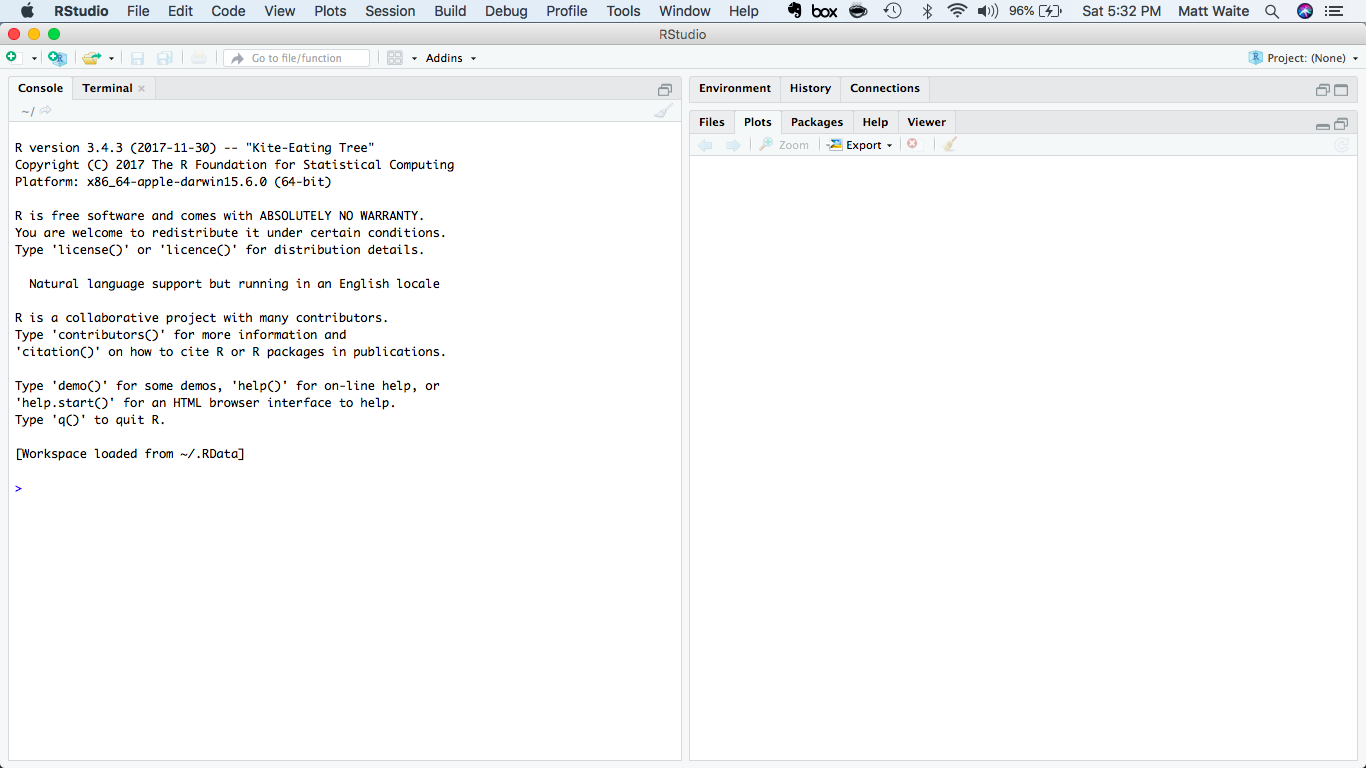
\includegraphics[width=18.97in]{images/verybasics1}

Think of the console like talking directly to R. It's direct, but it has some drawbacks and some quirks we'll get into later. For now, try typing this into the console and hit enter:

\begin{Shaded}
\begin{Highlighting}[]
\DecValTok{2}\OperatorTok{+}\DecValTok{2}
\end{Highlighting}
\end{Shaded}

\begin{verbatim}
## [1] 4
\end{verbatim}

Congrats, you've run some code. It's not very complex, and you knew the answer before hand, but you get the idea. We can compute things. We can also store things. \textbf{In programming languages, these are called variables}. We can assign things to variables using \texttt{\textless{}-}. And then we can do things with them. \textbf{The \texttt{\textless{}-} is a called an assignment operator}.

Try this in your console.

\begin{Shaded}
\begin{Highlighting}[]
\NormalTok{number <-}\StringTok{ }\DecValTok{2}

\NormalTok{number }\OperatorTok{*}\StringTok{ }\NormalTok{number}
\end{Highlighting}
\end{Shaded}

\begin{verbatim}
## [1] 4
\end{verbatim}

Now assign a different number to the variable number. Try run \texttt{number\ *\ number} again. Get what you expected?

We can have as many variables as we can name. \textbf{We can even reuse them (but be careful you know you're doing that or you'll introduce errors)}. Try this in your console.

\begin{Shaded}
\begin{Highlighting}[]
\NormalTok{firstnumber <-}\StringTok{ }\DecValTok{1}
\NormalTok{secondnumber <-}\StringTok{ }\DecValTok{2} 

\NormalTok{(firstnumber }\OperatorTok{+}\StringTok{ }\NormalTok{secondnumber) }\OperatorTok{*}\StringTok{ }\NormalTok{secondnumber}
\end{Highlighting}
\end{Shaded}

\begin{verbatim}
## [1] 6
\end{verbatim}

\textbf{We can store anything in a variable}. A whole table. An array of numbers. A single word. A whole book. All the books of the 18th century. They're really powerful. We'll explore them at length.

\hypertarget{adding-libraries-part-1}{%
\section{Adding libraries, part 1}\label{adding-libraries-part-1}}

The real strength of any given programming language is the external libraries that power it. The base language can do a lot, but it's the external libraries that solve many specific problems -- even making the base language easier to use.

For this class, we're going to need several external libraries.

The first library we're going to use is called Swirl. So in the console, type \texttt{install.packages(\textquotesingle{}swirl\textquotesingle{})} and hit enter. That installs swirl.

Now, to use the library, type \texttt{library(swirl)} and hit enter. That loads swirl. Then type \texttt{swirl()} and hit enter. Now you're running swirl. Follow the directions on the screen. When you are asked, you want to install course 1 R Programming: The basics of programming in R. Then, when asked, you want to do option 1, R Programming, in that course.

When you are finished with the course -- it will take just a few minutes -- type 0 to exit (it will not be clear that's what you do when you are done).

\hypertarget{adding-libraries-part-2}{%
\section{Adding libraries, part 2}\label{adding-libraries-part-2}}

We'll mostly use two libraries for analysis -- \texttt{dplyr} and \texttt{ggplot2}. To get them, and several other useful libraries, we can install a single collection of libraries called the tidyverse. Type this into your console: \texttt{install.packages(\textquotesingle{}tidyverse\textquotesingle{})}

\textbf{NOTE}: This is a pattern. You should always install libraries in the console.

Then, to help us with learning and replication, we're going to use R Notebooks. So we need to install that library. Type this into your console: \texttt{install.packages(\textquotesingle{}rmarkdown\textquotesingle{})}

\hypertarget{data-journalism-in-the-age-of-replication}{%
\chapter{Data journalism in the age of replication}\label{data-journalism-in-the-age-of-replication}}

It's a single word in a single job description, but a Buzzfeed job posting in 2017 is another indicator in what could be a profound shift in how data journalism is both practiced and taught.

``We're looking for someone with a passion for news and a commitment to using data to find amazing, important stories --- both quick hits and deeper analyses that drive conversations,'' the posting seeking a data journalist says. It goes on to list five things BuzzFeed is looking for: Excellent collaborator, clear writer, deep statistical understanding, knowledge of obtaining and restructuring data.

And then there's this:

\textbf{``You should have a strong command of at least one toolset that (a) allows for filtering, joining, pivoting, and aggregating tabular data, and (b) enables reproducible workflows.''}

The word you're seeing more and more of? Reproducible. And it started in earnest this summer when data journalism crossed a major threshold in American journalism: It now has it's own section in the Associated Press Stylebook.

``Data journalism has become a staple of reporting across beats and platforms,'' the Data Journalism section of the Stylebook opens. ``The ability to analyze quantitative information and present conclusions in an engaging and accurate way is no longer the domain of specialists alone.''

The AP's Data Journalism section discusses how to request data and in what format, guidelines for scraping data from websites with automation, the ethics of using leaked or hacked data and other topics long part of data journalism conference talks.

But the third page of the section contains perhaps the most profound commandment: \textbf{``As a general rule, all assertions in a story based on data analysis should be reproducible. The methodology description in the story or accompanying materials should provide a road map to replicate the analysis.''}

Reproducible research -- replication -- is a cornerstone of scientific inquiry. Researchers across a range of academic disciplines use methods to find new knowledge and publish it in peer reviewed journals. And, when it works, other researchers take that knowledge and try it with their own samples in their own locations. Replication studies exist to take something from an Interesting Finding to a Theory and beyond.

It doesn't always work.

Replication studies aren't funded at nearly the level as new research. And, to the alarm of many, scores of studies can't be replicated by others. Researchers across disciplines are finding that when their original studies are replicated, flaws are found, or the effects found aren't as strong as the original. Because of this, academics across a number of disciplines have written about a replication crisis in their respective fields, particularly psychology, social science and medical research.

In Chapter 1 of the New Precision Journalism, Phil Meyer wrote that ``we journalists would be wrong less often if we adapted to our own use some of the research tools of the social scientists.''

Meyer would go on to write about how computers pouring over datasets too large to crunch by hand had changed social science from a discipline with ``a few data and a lot of interpretation'' into a much more meaningful and powerful area of study. If journalists could become comfortable with data and some basic statistics, they too could harness this power.

``It used to be said that journalism is history in a hurry,'' Meyer wrote. ``The argument of this book is that to cope with the acceleration of social change in today's world, journalism must become social science in a hurry.''

He wrote that in 1971. It might as well have been yesterday.

Journalism doesn't have a history of replication, but the concerns about credibility are substantially greater. Trust in media is at an all time low and shows no signs of improving. While the politics of the day have quite a bit to do with this mistrust of media, being more transparent about what journalists do can't hurt.

The AP's commandment that Thou Must Replicate Your Findings could, if taken seriously by the news business, have substantial impacts on how data journalism gets done in newsrooms and how data journalism gets taught, both at professional conferences and universities.

How? Two ways.

\begin{itemize}
\tightlist
\item
  The predominant way that data journalism gets done in a newsroom is through simple tools like Microsoft Excel or Google Sheets. Those simple tools, on their own, lack significant logging functions, meaning journalists will have to maintain detailed logs of what they did so any analysis can be replicated.
\item
  The predominant way that data journalism gets taught -- both in professional settings and at most universities -- doesn't deal with replication at all. The tools and the training stress Getting Things Done -- an entirely logical focus for a deadline driven business. The choices of tools -- like spreadsheets -- are made to get from data to story as quick as possible, without frightening away math and tech phobic students.
\end{itemize}

If the AP's replication rules are to be followed, journalism needs to become much more serious about the tools and techniques used to do data journalism. The days of Point and Click tools to do Quick and Dirty analysis that get published are dying. The days of formal methods using documented steps are here.

\hypertarget{the-stylebook}{%
\section{The stylebook}\label{the-stylebook}}

Troy Thibodeaux, the editor of the AP's data journalism team, said the stylebook entry started when the data team found themselves answering the same questions over and over. With a grant from the Knight Foundation, the team began to document their own standards and turn that into a stylebook section.

From the beginning, they had a fairly clear idea of what they wanted to do -- think through a project and ask what the frequently asked questions are that came up. It was not going to be a soup-to-nuts guide to how to do a data project.

When the section came out, eyebrows went up on the replication parts, surprising Thibodeaux.

``From our perspective, this is a core value for us,'' he said. ``Just for our own benefit, we need to be able to have someone give us a second set of eyes. We benefit from that every day. We catch things for each other.''

Thibodeaux said the AP data team has two audiences when it comes to replication -- they have the readers of the work, and members of the collective who may want to do their own work with the data.

``This is something that's essential to the way we work,'' he said. ``And it's important in terms of transparency and credibility going forward. We thought it would be kind of unexceptionable.''

\hypertarget{replication}{%
\section{Replication}\label{replication}}

Meyer, now 86, said he's delighted to see replication up for discussion now, but warned that we shouldn't take it too far.

``Making the analysis replicable was something I worried about from the very beginning,'' he wrote in an email. So much so that in 1967, after publishing stories from his landmark survey after the Detroit riots, he shipped the data and backup materials about it to a social science data repository at the University of North Carolina.

And, in doing so, he opened the door to others replicating his results. One scholar attempted to find fault with Meyer's analysis by slicing the data ever thinner until the differences weren't significant -- gaming the analysis to criticize the stories.

Meyer believes replication is vitally important, but doesn't believe it should take on the trappings of science replication, where newsrooms take their own samples or re-survey a community. That would be prohibitively expensive.

But journalists should be sharing their data and analysis steps. And it doesn't need to be complicated, he said.

``Replication is a theoretical standard, not a requirement that every investigator duplicate his or her own work for every project,'' he said. ``Giving enough information in the report to enable another investigator to follow in your footsteps is enough. Just telling enough to make replication possible will build confidence.''

But as simple as that sounds, it's not so simple. Ask social scientists.

Andrew Gelman, a professor of statistics and political science and director of the Applied Statistics Center at Columbia University, wrote in the journal CHANCE in February that difficulties with replication in empirical research are pervasive.

``When an outsider requests data from a published paper, the authors will typically not post or send their data files and code, but instead will point to their sources, so replicators have to figure out exactly what to do from there,'' Gelman wrote. ``End-to-end replicability is not the norm, even among scholars who actively advocate for the principles of open science.''

So goes science, so goes journalism.

Until a recent set of exceptions, journalists rarely shared data. The ``nerd box'' -- a sidebar story that explains how a news organization did what they did -- is a term that first appeared on NICAR-L, a email listserv of data journalists, in the 1990s.

It was a form born in print.

As newsrooms adapted to the internet, some news organizations began linking to their data sources if they were online. Often, the data used in stories were obtained through records requests. Sometimes, reporters created the data themselves.

Journalism, more explicitly than science, is a competitive business. There have been arguments that nerd boxes and downloadable links give too much away to competitors.

Enter the AP Stylebook.

The AP Stylebook argues explicitly for both internal and external replication. Externally, they argue that the \textbf{``methodology description in the story or accompanying materials should provide a road map to replicate the analysis''}, meaning someone else could do the replication post publication.

Internally, the AP Stylebook says: \textbf{``If at all possible, an editor or another reporter should attempt to reproduce the results of the analysis and confirm all findings before publication.''}

There are two problems here.

First is that journalism, unlike science, has no history of replication. There is no Scientific Method for stories. There is no Research Methods class taught at every journalism school, at least not where it comes to writing stories. And, beyond that, journalism school isn't a requirement to get into the news business. In other words, journalism lacks the standards other disciplines have.

The second problem is, in many ways, worse: Except for the largest newsrooms, most news organizations lack editors who could replicate the analysis. Many don't have a second person who would know what to do.

Not having a second set of eyes in a newsroom is a problem, Thibodeaux acknowledges. Having a data journalism team ``is an incredible luxury'' at the AP, he said, and their rule is nothing goes on the wire without a second set of eyes.

Thibodeaux, for his part, wants to see fewer ``lone nerds in the corner'' -- it's too much pressure. That person gets too much credibility from people who don't understand what they do, and they get too much blame when a mistake is made.

So what would replication look like in a newsroom? What does this mean for how newsrooms do data journalism on deadline? And what does this mean for how data journalism is being taught, particularly at a time when only half of accredited journalism programs teach any data journalism at all?

Are we walking ourselves into our own replication crisis?

\hypertarget{goodbye-excel}{%
\section{Goodbye Excel?}\label{goodbye-excel}}

For decades, Excel has been the gateway drug for data journalists, the Swiss Army knife of data tools, the One Tool You Can't Live Without. Investigative Reporters and Editors, an organization that trains investigative journalists, have built large amounts of their curricula around Excel. Of the journalism schools that teach data journalism, most of them begin and end with spreadsheets.

The Stylebook says at a minimum, today's data journalists should keep a log that details:

\begin{itemize}
\tightlist
\item
  The source of the data, making sure to work on a copy of the data and not the original file.
\item
  Data dictionaries or any other supporting documentation of the data.
\item
  \textbf{``Description of all steps required to transform the data and perform the analysis.''}
\end{itemize}

The trouble with Excel is, unless you are keeping meticulous notes on what steps you are taking, there's no way to keep track. Many data journalists will copy and paste the values of a formula over the formula itself to prevent Excel from fouling up cell references when moving data around -- a practical step that also cuts off another path to being able to replicate the results.

An increasing number of data journalists are switching to tools like analysis notebooks, which use languages like Python and R, to document their work. The notebooks, generally speaking, allow a data journalist to mix code and explanation in the same document.

Combined with online sharing tools like GitHub, analysis notebooks seem to solve the problem of replication. But the number using them is small compared to those using spreadsheets. Recent examples of news organizations using analysis notebooks include the \href{https://github.com/datadesk}{Los Angeles Times}, the \href{https://github.com/TheUpshot}{New York Times}, \href{https://github.com/fivethirtyeight/data}{FiveThirtyEight}, and \href{https://github.com/BuzzFeedNews}{Buzzfeed}.

Peter Aldous, a data journalist at Buzzfeed recently published a story about how the online news site used machine learning to find airplanes being used to spy on people in American cities. Published with the story is the code Aldous used to build his case.

``I think of it this way: As a journalist, I don't like to simply trust what people tell me. Sometimes sources lie. Sometimes they're just mistaken. So I like to verify what I'm told,'' he wrote in an email. ``By the same token, why should someone reading one of my articles believe my conclusions, if I don't provide the evidence that explains how I reached them?''

The methodology document, associated code and source data took Aldous a few hours to create. The story, from the initial data work through the reporting required to make sense of it all, took a year. Aldous said there wasn't a discussion about if the methodology would be published because it was assumed -- ``it's written into our DNA at BuzzFeed News.''

``My background is in science journalism, and before that (way back in the 1980s) in science,'' Aldous said. ``In science, there's been a shift from descriptive methods sections to publishing data and analysis code for reproducible research. And I think we're seeing a similar shift in data journalism. Simply saying what you've done is not as powerful as providing the means for others to repeat and build on your work.''

Thibodeaux said that what Buzzfeed and others do with analysis notebooks and code repositories that include their data is ``lovely.''

``That to me is the shining city on the hill,'' Thibodeaux said. ``We're not going to get there, and I don't think we have to for every story and every use case, and I don't think it's necessarily practical for every person working with data to get to that point.''

There's a wide spectrum of approaches that still gets journalists to the essence of what the stylebook is trying to do, Thibodeaux said. There are many tools, many strategies, and the AP isn't going to advocate for any single one of them, he said. They're just arguing for transparency and replicability, even if that means doing more work.

``There's a certain burden that comes with transparency,'' he said. ``And I think we have to accept that burden.''

The question, Thibodeaux said, is what is sufficient? What's enough transparency? What does someone need for replicability?

``Maybe we do have to set a higher standard -- the more critical the analysis is to the story, and the more complex that analysis is, that's going to push the bar on what is a sufficient methodology statement,'' he said. ``And it could end up being a whole code repo in order to just say, this isn't black magic, here's how we got it if you're so interested.''

\hypertarget{receptivity-is-high}{%
\section{``Receptivity \ldots{} is high''}\label{receptivity-is-high}}

Though written almost half a century ago, Meyer foresaw how data journalism was going to arrive in the newsroom.

``For the new methods to gain currency in journalism, two things must happen,'' he wrote. ``Editors must feel the need strongly enough to develop the in-house capacity for systematic research \ldots{} The second need, of course, is for the editors to be able to find the talent to fill this need.''

Meyer optimistically wrote that journalism schools were prepared to provide that talent -- they were not then, and only small handful are now -- but students were unlikely to be drawn to these new skills if they didn't see a chance to use those skills in their careers.

It's taken 45 years, but we are now at this point.

``The potential for receptivity, especially among the younger generation of newspaper managers, is high,'' Meyer wrote.

\hypertarget{replication-in-notebooks}{%
\section{Replication in notebooks}\label{replication-in-notebooks}}

For our purposes in this book, replication requires two things from you, the student: What and why. What is this piece of code doing, and why are you doing that here and now? What lead you to this place? That you can copy and paste code from this book or the internet is not impressive. What is necessary for learning is that you know what a piece of code is doing a thing and why you want to do that thing here.

In an R Notebook, there are two blocks: A block that uses markdown, which has no special notation, and a code block. The code blocks can run mulitple languages inside R Studio, including Python, a general purpose scripting language; and SQL, or Structured Query Language, the language of databases.

For the rest of the class, we're going to be working in notebooks. In notebooks, you will both run your code and explain each step, much as I am doing here.

To start a notebook, you click on the green plus in the top left corner and go down to R Notebook. Do that now.

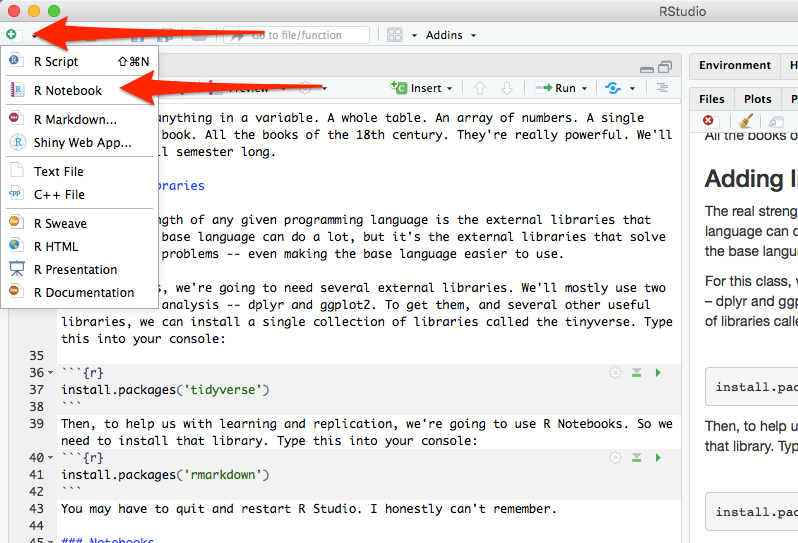
\includegraphics[width=11.08in]{images/verybasics2}

You will see that the notebook adds a lot of text for you. It tells you how to work in notebooks -- and you should read it. The most important parts are these:

To add text, simply type. To add code you can click on the \emph{Insert} button on the toolbar or by pressing \emph{Cmd+Option+I} on Mac or \emph{Ctl+Alt+I} on Windows.

Highlight all that text and delete it. You should have a blank document. This document is called a R Markdown file -- it's a special form of text, one that you can style, and one you can include R in the middle of it. Markdown is a simple markup format that you can use to create documents. So first things first, let's give our notebook a big headline. Add this:

\texttt{\#\ My\ awesome\ notebook}

Now, under that, without any markup, just type This is my awesome notebook.

Under that, you can make text bold by writing \texttt{It\ is\ **really**\ awesome}.

If you want it italics, just do this on the next line: \texttt{No,\ it\textquotesingle{}s\ \_really\_\ awesome.\ I\ swear.}

To see what it looks like without the markup, click the Preview or Knit button in the toolbar. That will turn your notebook into a webpage, with the formatting included.

Throughout this book, we're going to use this markdown to explain what we are doing and, more importantly, why we are doing it. Explaining your thinking is a vital part of understanding what you are doing.

That explaination, plus the code, is the real power of notebooks. To add a block of code, follow the instructions from above: click on the \emph{Insert} button on the toolbar or by pressing \emph{Cmd+Option+I} on Mac or \emph{Ctl+Alt+I} on Windows.

In that window, use some of the code from above and add two numbers together. To see it run, click the green triangle on the right. That runs the chunk. You should see the answer to your addition problem.

And that, just that, is the foundation you need to start this book.

\hypertarget{data-structures-and-types}{%
\chapter{Data, structures and types}\label{data-structures-and-types}}

Data are everywhere (and data is plural of datum, thus the use of are in that statement). It surrounds you. Every time you use your phone, you are creating data. Lots of it. Your online life. Any time you buy something. It's everywhere. News, like life, is no different. Modernity is drowning in data, and more comes along all the time.

In news, and in this class, we'll be dealing largely with two kinds of data: \textbf{event level data and summary data}. It's not hard to envision event level data. A car accident. A crime. A fire. They are the events that make up the whole. Combine them together -- summarize them -- and you'll have some notion of how the year went. What we usually see is summary data -- who wants to scroll through 365 days of crime data to figure out if crime was up or down?

To start with, we need to understand the shape of data.

\hypertarget{rows-and-columns}{%
\section{Rows and columns}\label{rows-and-columns}}

Data, oversimplifying it a bit, is information organized. Generally speaking, it's organized into rows and columns. Rows, generally, are individual elements. A crime. A county. An accident. Columns, generally, are components of the data, sometimes called variables. So if each row is a crime, the first column might be the type. The second is the date and time. The third is the location. And so on.

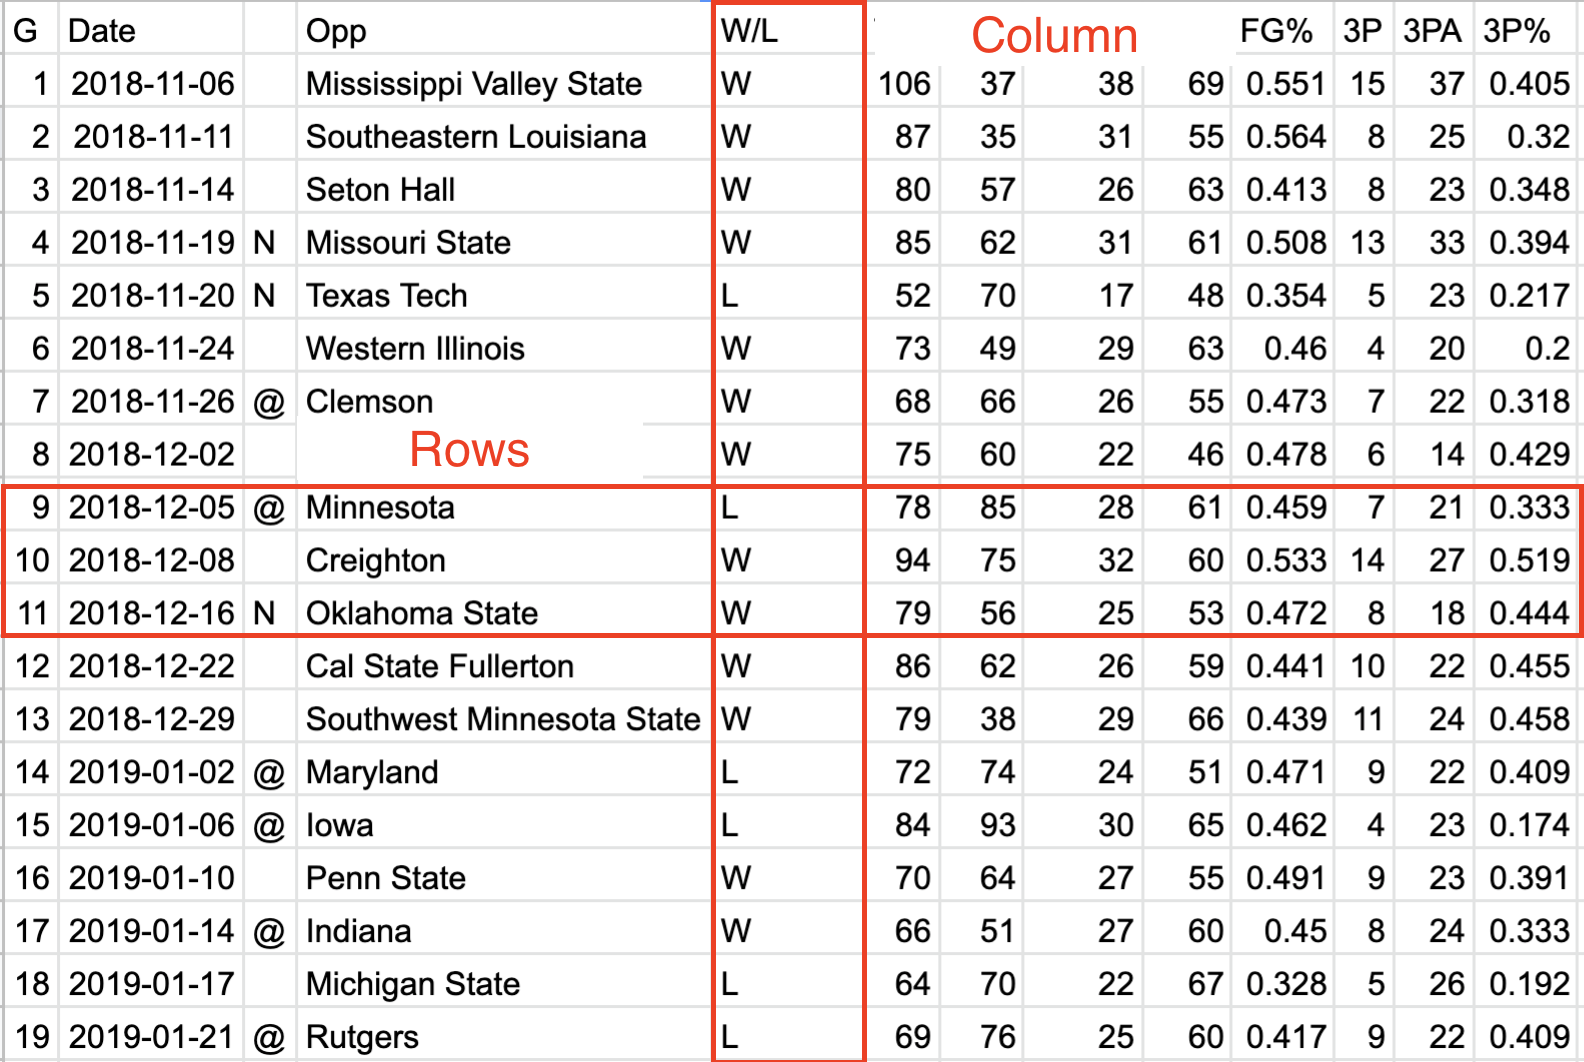
\includegraphics[width=22in]{images/data1}

One of the critical components of data analysis, especially for beginners, is having a mental picture of your data. What does each row mean? What does each column in each row signify? How many rows do you have? How many columns?

\begin{quote}
EXERCISE: I love orange Skittles. What are my chances of getting more orange Skittles than other colors in a fun sized packet? Each person in the class must track their package and everyone else using a spreadsheet. What differences between sheets emerge? What similarities?
\end{quote}

\hypertarget{types}{%
\section{Types}\label{types}}

There are scores of data types in the world, and R has them. In this class, we're primarily going to be dealing with data frames, and each element of our data frames will have a data type.

Typically, they'll be one of four types of data:

\begin{itemize}
\tightlist
\item
  Numeric: a number, like the number of car accidents in a year or the number of journalism majors.
\item
  Character: Text, like a name, a county, a state.
\item
  Date: Fully formed dates -- 2019-01-01 -- have a special date type. Elements of a date, like a year (ex. 2019) are not technically dates, so they'll appear as numeric data types.
\item
  Logical: Rare(ish), but every now and then we'll have a data type that's Yes or No, True or False, etc.
\end{itemize}

\textbf{Question:} Is a zip code a number? Is a jersey number a number? Trick question, because the answer is no. Numbers are things we do math on. If the thing you want is not something you're going to do math on -- can you add two phone numbers together? -- then make it a character type. If you don't, most every software system on the planet will drop leading zeros. For example, every zip code in Boston starts with 0. If you record that as a number, your zip code will become a four digit number, which isn't a zip code anymore.

\hypertarget{a-simple-way-to-get-data}{%
\section{A simple way to get data}\label{a-simple-way-to-get-data}}

The hardest part of doing data journalism is often getting the data. In news, there's scores of organizations and agencies collecting data, and zero standards on how it's being collected.

If we're lucky -- huge IF in news -- the data we want is in a downloadable format. If we're a little less lucky, there's a way to get the data on the web. And maybe that data is in a simple table. If so, we can pull that data directly into Google Sheets.

The Lincoln Police Department publishes a daily summary of calls. Some days -- like when it snows -- that data becomes news. So let's pretend that it snowed today and we need to see how many accidents the Lincoln Police responded to and what percentage of their call load that represents.

Open a browser and go to the \href{http://cjis.lincoln.ne.gov/~lpd/cfstoday.htm}{LPD's log page}. Now, in a new tab, log into Google Docs/Drive and open a new spreadsheet. In the first cell of the first row, copy and paste this formula in:

\begin{verbatim}
=importHTML("http://cjis.lincoln.ne.gov/~lpd/cfstoday.htm","table",1)
\end{verbatim}

This is \textbf{function}, with three \textbf{inputs}. The function is \texttt{importHTML} and the three inputs in order are the url of the page, the HTML tag we're after (a

tag in our case) and the number of the tag you're after. So our function says go to the LPD page and get the first table tag you find. Fortunately for us, there's only one.

If your version worked right, you've got the data from that page in a spreadsheet.

\hypertarget{cleaning-the-data}{%
\section{Cleaning the data}\label{cleaning-the-data}}

The first thing we need to do is recognize that we don't have data, really. We have the results of a formula. You can tell by putting your cursor on that field, where you'll see the formula again. This is where you'd look:

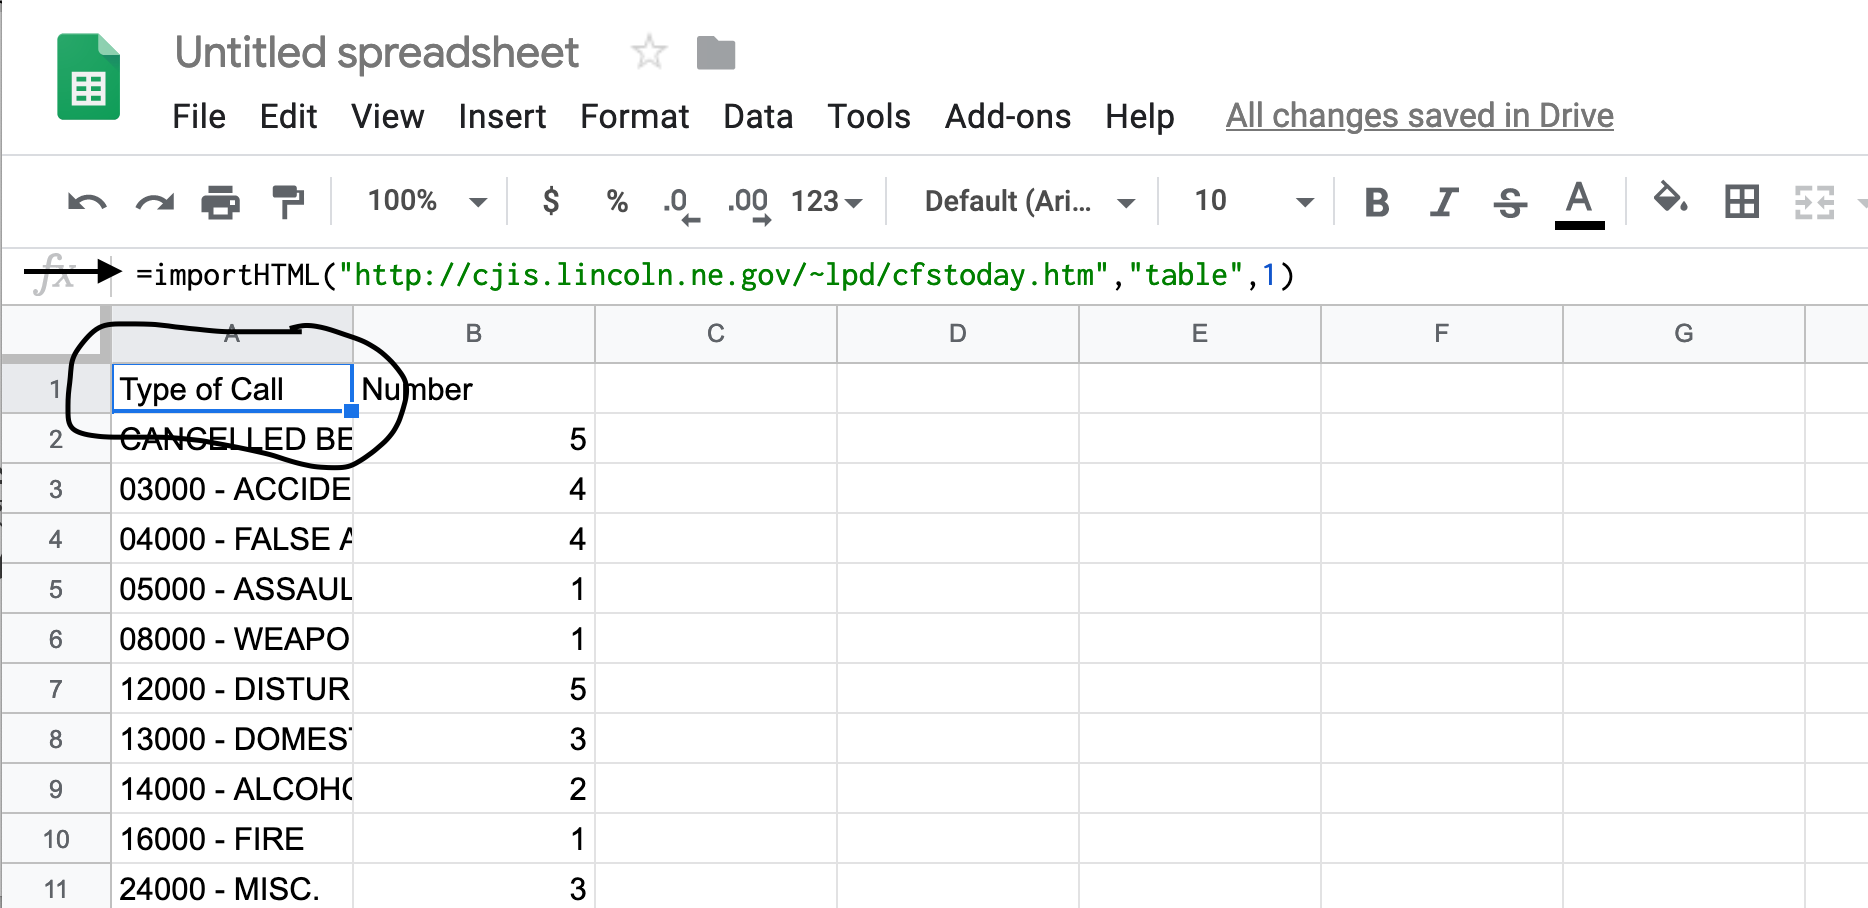
\includegraphics[width=25.94in]{images/clean1}

The solution is easy:

Edit \textgreater{} Select All or type command/control A
Edit \textgreater{} Copy or type command/control C
Edit \textgreater{} Paste Special \textgreater{} Values Only or type command/control shift V

You can verify that it worked by looking in that same row 1 column A, where you'll see the formula is gone.

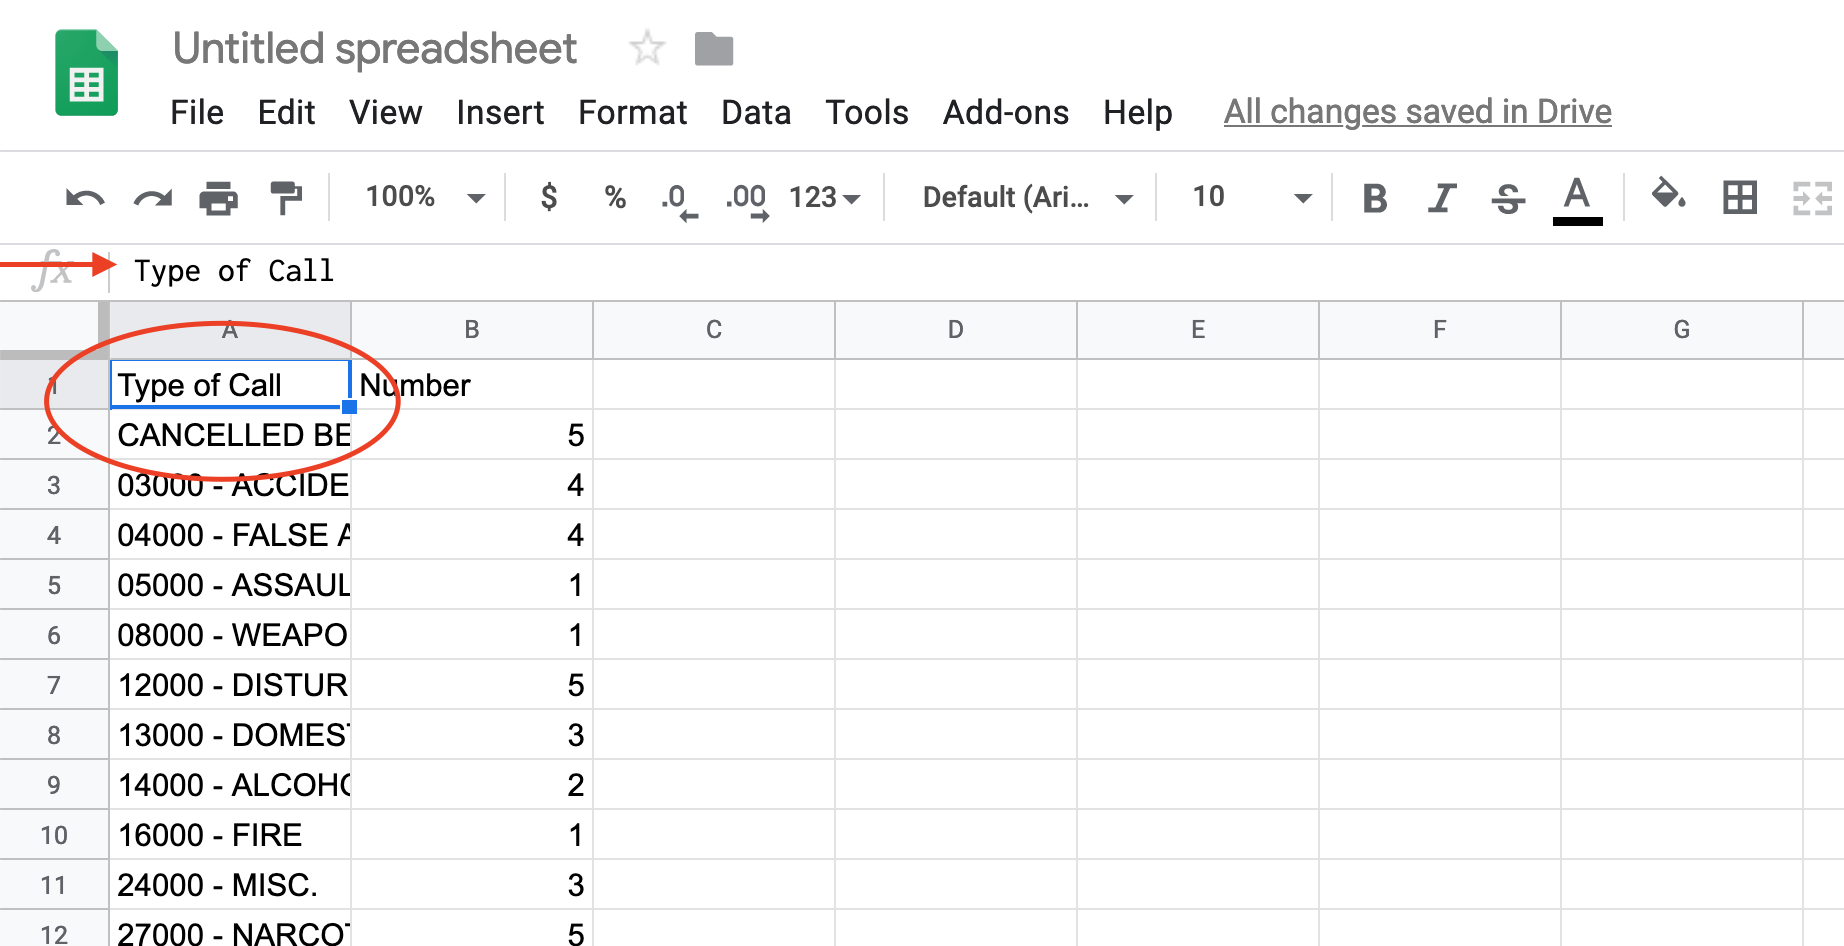
\includegraphics[width=25.61in]{images/clean2}

Now you have data, but look closely. At the bottom of the data, you have the total number of calls. More often than not, and particularly the deeper into this book we go, you want to delete that. So click on the number next to that Total Calls line to highlight it and go up to Edit \textgreater{} Delete Row XX where XX is the row number.

After you've done that, you can export it for use in R. Go to File \textgreater{} Download as \textgreater{} Comma Separated Values.

\hypertarget{aggregates}{%
\chapter{Aggregates}\label{aggregates}}

R is a statistical programming language that is purpose built for data analysis.

Base R does a lot, but there are a mountain of external libraries that do things to make R better/easier/more fully featured. We already installed the tidyverse -- or you should have if you followed the instructions for the last assignment -- which isn't exactly a library, but a collection of libraries. Together, they make up the tidyverse. Individually, they are extraordinarily useful for what they do. We can load them all at once using the tidyverse name, or we can load them individually. Let's start with individually.

The two libraries we are going to need for this assignment are \texttt{readr} and \texttt{dplyr}. The library \texttt{readr} reads different types of data in. For this assignment, we're going to read in csv data or Comma Separated Values data. That's data that has a comma between each column of data.

Then we're going to use \texttt{dplyr} to analyze it.

To use a library, you need to import it. Good practice -- one I'm going to insist on -- is that you put all your library steps at the top of your notebooks.

That code looks like this:

\begin{Shaded}
\begin{Highlighting}[]
\KeywordTok{library}\NormalTok{(readr)}
\end{Highlighting}
\end{Shaded}

To load them both, you need to do this:

\begin{Shaded}
\begin{Highlighting}[]
\KeywordTok{library}\NormalTok{(readr)}
\KeywordTok{library}\NormalTok{(dplyr)}
\end{Highlighting}
\end{Shaded}

But, because those two libraries -- and several others that we're going to use over the course of this class -- are so commonly used, there's a shortcut to loading all of the libraries we'll need:

\begin{Shaded}
\begin{Highlighting}[]
\KeywordTok{library}\NormalTok{(tidyverse)}
\end{Highlighting}
\end{Shaded}

You can keep doing that for as many libraries as you need. I've seen notebooks with 10 or more library imports.

\hypertarget{importing-data}{%
\section{Importing data}\label{importing-data}}

The first thing we need to do is get some data to work with. We do that by reading it in. In our case, we're going to read data from a csv file -- a comma-separated values file.

The CSV file we're going to read from is a \href{https://unl.box.com/s/xjipgkesl9rjmng4weg77vb73xt41apf}{Nebraska Game and Parks Commission dataset} of confirmed mountain lion sightings in Nebraska. There are, on occasion, fierce debates about mountain lions and if they should be hunted in Nebraska. This dataset can tell us some interesting things about that debate.

So step 1 is to import the data. The code looks \emph{something} like this, but hold off copying it just yet:

\texttt{mountainlions\ \textless{}-\ read\_csv("\textasciitilde{}/Documents/Data/mountainlions.csv")}

Let's unpack that.

The first part -- mountainlions -- is the name of your variable. A variable is just a name of a thing. In this case, our variable is a dataframe, which is R's way of storing data. We can call this whatever we want. I always want to name dataframes after what is in it. In this case, we're going to import a dataset of mountain lion sightings from the Nebraska Game and Parks Commission. \textbf{Variable names, by convention are one word all lower case}. You can end a variable with a number, but you can't start one with a number.

The \textless{}- bit, you'll recall from the basics, is the \textbf{variable assignment operator}. It's how we know we're assigning something to a word. Think of the arrow as saying ``Take everything on the right of this arrow and stuff it into the thing on the left.'' So we're creating an empty vessel called mountainlions and stuffing all this data into it.

The \texttt{read\_csv} bits are pretty obvious, except for one thing. What happens in the quote marks is the path to the data. In there, I have to tell R where it will find the data.

\begin{quote}
The easiest thing to do, if you are confused about how to find your data, is to put your data in the same folder as as your notebook (you'll have to save that notebook first). If you do that, then you just need to put the name of the file in there (mountainlions.csv).
\end{quote}

In my case, the file path I've got starts with a \textasciitilde{} character. That's a shortcut for my home directory. It's the same on your computer. Your home directory is where your Documents, Desktop and Downloads directories are. I've got a folder called Documents in my home directory, and in there is a folder called Data that has the file called mountainlions.csv in it. Thus, \texttt{\textasciitilde{}/Documents/Data/mountainlions.csv}

Some people -- insane people -- leave the data in their downloads folder. The data path then would be \texttt{\textasciitilde{}/Downloads/nameofthedatafilehere.csv} on PC or Mac.

A quick way to find your data file? The tab key. If you start your code \texttt{dataframenamehere\ \textless{}-\ read\_csv(")} and after typing the first quote mark you hit tab, it will show you the files in the folder you are in. With that, you can start to narrow in on where you need to go.

\textbf{So what you put in your import step will be different from mine}. Your first task is to import the data. Here's mine. Use the tab key to find your data file and get the correct path.

\begin{Shaded}
\begin{Highlighting}[]
\NormalTok{mountainlions <-}\StringTok{ }\KeywordTok{read_csv}\NormalTok{(}\StringTok{"data/mountainlions.csv"}\NormalTok{)}
\end{Highlighting}
\end{Shaded}

\begin{verbatim}
## Parsed with column specification:
## cols(
##   ID = col_double(),
##   `Cofirm Type` = col_character(),
##   COUNTY = col_character(),
##   Date = col_character()
## )
\end{verbatim}

Now we can inspect the data we imported. What does it look like? To do that, we use \texttt{head(mountainlions)} to \textbf{show the headers and the first six rows of data}. If we wanted to see them all, we could just simply enter \texttt{mountainlions} and run it.

To get the number of records in our dataset, we run \texttt{nrow(mountainlions)}

\begin{Shaded}
\begin{Highlighting}[]
\KeywordTok{head}\NormalTok{(mountainlions)}
\end{Highlighting}
\end{Shaded}

\begin{verbatim}
## # A tibble: 6 x 4
##      ID `Cofirm Type` COUNTY       Date    
##   <dbl> <chr>         <chr>        <chr>   
## 1     1 Track         Dawes        9/14/91 
## 2     2 Mortality     Sioux        11/10/91
## 3     3 Mortality     Scotts Bluff 4/21/96 
## 4     4 Mortality     Sioux        5/9/99  
## 5     5 Mortality     Box Butte    9/29/99 
## 6     6 Track         Scotts Bluff 11/12/99
\end{verbatim}

\begin{Shaded}
\begin{Highlighting}[]
\KeywordTok{nrow}\NormalTok{(mountainlions)}
\end{Highlighting}
\end{Shaded}

\begin{verbatim}
## [1] 393
\end{verbatim}

\hypertarget{group-by-and-count}{%
\section{Group by and count}\label{group-by-and-count}}

So what if we wanted to know how many mountain lion sightings there were in each county?

To do that by hand, we'd have to take each of the 393 records and sort them into a pile. We'd put them in groups and then count them.

\texttt{dplyr} has a group by function in it that does just this. A massive amount of data analysis involves grouping like things together and then doing simple things like counting them, or averaging them together. So it's a good place to start.

So to do this, we'll take our dataset and we'll introduce a new operator: \texttt{\%\textgreater{}\%}. The best way to read that operator, in my opinion, is to interpret that as ``and then do this.''

We're going to establish a pattern that will come up again and again throughout this book: \texttt{data\ \%\textgreater{}\%\ function}. The first step of every analysis starts with the data being used. Then we apply functions to the data.

In our case, the pattern that you'll use many, many times is: \texttt{data\ \%\textgreater{}\%\ group\_by(FIELD\ NAME)\ \%\textgreater{}\%\ summarize(VARIABLE\ NAME\ =\ AGGREGATE\ FUNCTION(FIELD\ NAME))}

Here's the code:

\begin{Shaded}
\begin{Highlighting}[]
\NormalTok{mountainlions }\OperatorTok
\StringTok{  }\KeywordTok{group_by}\NormalTok{(COUNTY) }\OperatorTok
\StringTok{  }\KeywordTok{summarise}\NormalTok{(}
    \DataTypeTok{total =} \KeywordTok{n}\NormalTok{()}
\NormalTok{  )}
\end{Highlighting}
\end{Shaded}

\begin{verbatim}
## # A tibble: 42 x 2
##    COUNTY    total
##    <chr>     <int>
##  1 Banner        6
##  2 Blaine        3
##  3 Box Butte     4
##  4 Brown        15
##  5 Buffalo       3
##  6 Cedar         1
##  7 Cherry       30
##  8 Custer        8
##  9 Dakota        3
## 10 Dawes       111
## # ... with 32 more rows
\end{verbatim}

So let's walk through that. We start with our dataset -- \texttt{mountainlions} -- and then we tell it to group the data by a given field in the data. In this case, we wanted to group together all the counties, signified by the field name COUNTY, which you could get from looking at \texttt{head(mountainlions)}. After we group the data, we need to count them up. In dplyr, we use \texttt{summarize} \href{http://dplyr.tidyverse.org/reference/summarise.html}{which can do more than just count things}. Inside the parentheses in summarize, we set up the summaries we want. In this case, we just want a count of the counties: \texttt{total\ =\ n(),} says create a new field, called \texttt{total} and set it equal to \texttt{n()}, which might look weird, but it's common in stats. The number of things in a dataset? Statisticians call in n. There are n number of incidents in this dataset. So \texttt{n()} is a function that counts the number of things there are.

And when we run that, we get a list of counties with a count next to them. But it's not in any order. So we'll add another And Then Do This \%\textgreater{}\% and use \texttt{arrange}. Arrange does what you think it does -- it arranges data in order. By default, it's in ascending order -- smallest to largest. But if we want to know the county with the most mountain lion sightings, we need to sort it in descending order. That looks like this:

\begin{Shaded}
\begin{Highlighting}[]
\NormalTok{mountainlions }\OperatorTok
\StringTok{  }\KeywordTok{group_by}\NormalTok{(COUNTY) }\OperatorTok
\StringTok{  }\KeywordTok{summarise}\NormalTok{(}
    \DataTypeTok{count =} \KeywordTok{n}\NormalTok{()}
\NormalTok{  ) }\OperatorTok\StringTok{ }\KeywordTok{arrange}\NormalTok{(}\KeywordTok{desc}\NormalTok{(count))}
\end{Highlighting}
\end{Shaded}

\begin{verbatim}
## # A tibble: 42 x 2
##    COUNTY       count
##    <chr>        <int>
##  1 Dawes          111
##  2 Sioux           52
##  3 Sheridan        35
##  4 Cherry          30
##  5 Scotts Bluff    26
##  6 Keya Paha       20
##  7 Brown           15
##  8 Rock            11
##  9 Lincoln         10
## 10 Custer           8
## # ... with 32 more rows
\end{verbatim}

We can, if we want, group by more than one thing. So how are these sightings being confirmed? To do that, we can group by County and ``Cofirm Type'', which is how the state misspelled Confirm. But note something in this example below:

\begin{Shaded}
\begin{Highlighting}[]
\NormalTok{mountainlions }\OperatorTok
\StringTok{  }\KeywordTok{group_by}\NormalTok{(COUNTY, }\StringTok{`}\DataTypeTok{Cofirm Type}\StringTok{`}\NormalTok{) }\OperatorTok
\StringTok{  }\KeywordTok{summarise}\NormalTok{(}
    \DataTypeTok{count =} \KeywordTok{n}\NormalTok{()}
\NormalTok{  ) }\OperatorTok\StringTok{ }\KeywordTok{arrange}\NormalTok{(}\KeywordTok{desc}\NormalTok{(count))}
\end{Highlighting}
\end{Shaded}

\begin{verbatim}
## # A tibble: 93 x 3
## # Groups:   COUNTY [42]
##    COUNTY       `Cofirm Type`      count
##    <chr>        <chr>              <int>
##  1 Dawes        Trail Camera Photo    41
##  2 Sioux        Trail Camera Photo    40
##  3 Dawes        Track                 19
##  4 Keya Paha    Trail Camera Photo    18
##  5 Cherry       Trail Camera Photo    17
##  6 Dawes        Mortality             17
##  7 Sheridan     Trail Camera Photo    16
##  8 Dawes        Photo                 13
##  9 Dawes        DNA                   11
## 10 Scotts Bluff Trail Camera Photo    11
## # ... with 83 more rows
\end{verbatim}

See it? When you have a field name that has two words, \texttt{readr} wraps it in back ticks, which is next to the 1 key on your keyboard. You can figure out which fields have back ticks around it by looking at the output of \texttt{readr}. Pay attention to that, because it's coming up again in the next section and will be a part of your homework.

\hypertarget{other-aggregates-mean-and-median}{%
\section{Other aggregates: Mean and median}\label{other-aggregates-mean-and-median}}

In the last example, we grouped some data together and counted it up, but there's so much more you can do. You can do multiple measures in a single step as well.

Let's look at some \href{https://unl.box.com/s/09t2u4qoncfh6qlv2156flzlxb8ruzpq}{salary data from the University of Nebraska}.

\begin{Shaded}
\begin{Highlighting}[]
\NormalTok{salaries <-}\StringTok{ }\KeywordTok{read_csv}\NormalTok{(}\StringTok{"data/nusalaries1819.csv"}\NormalTok{)}
\end{Highlighting}
\end{Shaded}

\begin{verbatim}
## Parsed with column specification:
## cols(
##   Employee = col_character(),
##   Position = col_character(),
##   Campus = col_character(),
##   Department = col_character(),
##   `Budgeted Annual Salary` = col_number(),
##   `Salary from State Aided Funds` = col_number(),
##   `Salary from Other Funds` = col_number()
## )
\end{verbatim}

\begin{Shaded}
\begin{Highlighting}[]
\KeywordTok{head}\NormalTok{(salaries)}
\end{Highlighting}
\end{Shaded}

\begin{verbatim}
## # A tibble: 6 x 7
##   Employee Position Campus Department `Budgeted Annua~ `Salary from St~
##   <chr>    <chr>    <chr>  <chr>                 <dbl>            <dbl>
## 1 Abbey, ~ Associa~ UNK    Kinesiolo~            61276            61276
## 2 Abbott,~ Staff S~ UNL    FM&P Faci~            37318               NA
## 3 Abboud,~ Adminis~ UNMC   Surgery-U~            76400            76400
## 4 Abdalla~ Asst Pr~ UNMC   Pathology~            74774            71884
## 5 Abdelka~ Post-Do~ UNMC   Surgery-T~            43516               NA
## 6 Abdel-M~ Researc~ UNL    Public Po~            58502               NA
## # ... with 1 more variable: `Salary from Other Funds` <dbl>
\end{verbatim}

In summarize, we can calculate any number of measures. Here, we'll use R's built in mean and median functions to calculate \ldots{} well, you get the idea.

\begin{Shaded}
\begin{Highlighting}[]
\NormalTok{salaries }\OperatorTok
\StringTok{  }\KeywordTok{summarise}\NormalTok{(}
    \DataTypeTok{count =} \KeywordTok{n}\NormalTok{(),}
    \DataTypeTok{mean_salary =} \KeywordTok{mean}\NormalTok{(}\StringTok{`}\DataTypeTok{Budgeted Annual Salary}\StringTok{`}\NormalTok{),}
    \DataTypeTok{median_salary =} \KeywordTok{median}\NormalTok{(}\StringTok{`}\DataTypeTok{Budgeted Annual Salary}\StringTok{`}\NormalTok{)}
\NormalTok{  )}
\end{Highlighting}
\end{Shaded}

\begin{verbatim}
## # A tibble: 1 x 3
##   count mean_salary median_salary
##   <int>       <dbl>         <dbl>
## 1 13039      62065.         51343
\end{verbatim}

So there's 13,039 employees in the database, spread across four campuses plus the system office. The mean or average salary is about \$62,000, but the median salary is slightly more than \$51,000.

Why?

Let's let sort help us.

\begin{Shaded}
\begin{Highlighting}[]
\NormalTok{salaries }\OperatorTok\StringTok{ }\KeywordTok{arrange}\NormalTok{(}\KeywordTok{desc}\NormalTok{(}\StringTok{`}\DataTypeTok{Budgeted Annual Salary}\StringTok{`}\NormalTok{))}
\end{Highlighting}
\end{Shaded}

\begin{verbatim}
## # A tibble: 13,039 x 7
##    Employee Position Campus Department `Budgeted Annua~ `Salary from St~
##    <chr>    <chr>    <chr>  <chr>                 <dbl>            <dbl>
##  1 Frost, ~ Head Co~ UNL    Athletics           5000000               NA
##  2 Miles, ~ Head Co~ UNL    Athletics           2375000               NA
##  3 Moos, W~ Athleti~ UNL    Athletics           1000000               NA
##  4 Gold, J~ Chancel~ UNMC   Office of~           853338           853338
##  5 Chinand~ Assista~ UNL    Athletics            800000               NA
##  6 Walters~ Assista~ UNL    Athletics            700000               NA
##  7 Cook, J~ Head Co~ UNL    Athletics            675000               NA
##  8 William~ Head Co~ UNL    Athletics            626750               NA
##  9 Bounds,~ Preside~ UNCA   Office of~           540000           540000
## 10 Austin ~ Assista~ UNL    Athletics            475000               NA
## # ... with 13,029 more rows, and 1 more variable: `Salary from Other
## #   Funds` <dbl>
\end{verbatim}

Oh, right. In this dataset, the university pays a football coach \$5 million. Extremes influence averages, not medians, and now you have your answer.

So when choosing a measure of the middle, you have to ask yourself -- could I have extremes? Because a median won't be sensitive to extremes. It will be the point at which half the numbers are above and half are below. The average or mean will be a measure of the middle, but if you have a bunch of low paid people and then one football coach, the average will be wildly skewed. Here, because there's so few highly paid football coaches compared to people who make a normal salary, the number is only slightly skewed in the grand scheme, but skewed nonetheless.

\hypertarget{even-more-aggregates}{%
\section{Even more aggregates}\label{even-more-aggregates}}

There's a ton of things we can do in summarize -- we'll work with more of them as the course progresses -- but here's a few other questions you can ask.

Which department on campus has the highest wage bill? And what is the highest and lowest salary in the department? And how wide is the spread between salaries? We can find that with \texttt{sum} to add up the salaries to get the total wage bill, \texttt{min} to find the minumum salary, \texttt{max} to find the maximum salary and \texttt{sd} to find the standard deviation in the numbers.

\begin{Shaded}
\begin{Highlighting}[]
\NormalTok{salaries }\OperatorTok\StringTok{ }
\StringTok{  }\KeywordTok{group_by}\NormalTok{(Campus, Department) }\OperatorTok\StringTok{ }
\StringTok{  }\KeywordTok{summarize}\NormalTok{(}
    \DataTypeTok{total =} \KeywordTok{sum}\NormalTok{(}\StringTok{`}\DataTypeTok{Budgeted Annual Salary}\StringTok{`}\NormalTok{), }
    \DataTypeTok{avgsalary =} \KeywordTok{mean}\NormalTok{(}\StringTok{`}\DataTypeTok{Budgeted Annual Salary}\StringTok{`}\NormalTok{), }
    \DataTypeTok{minsalary =} \KeywordTok{min}\NormalTok{(}\StringTok{`}\DataTypeTok{Budgeted Annual Salary}\StringTok{`}\NormalTok{),}
    \DataTypeTok{maxsalary =} \KeywordTok{max}\NormalTok{(}\StringTok{`}\DataTypeTok{Budgeted Annual Salary}\StringTok{`}\NormalTok{),}
    \DataTypeTok{stdev =} \KeywordTok{sd}\NormalTok{(}\StringTok{`}\DataTypeTok{Budgeted Annual Salary}\StringTok{`}\NormalTok{)) }\OperatorTok\StringTok{ }\KeywordTok{arrange}\NormalTok{(}\KeywordTok{desc}\NormalTok{(total))}
\end{Highlighting}
\end{Shaded}

\begin{verbatim}
## # A tibble: 804 x 7
## # Groups:   Campus [5]
##    Campus Department                  total avgsalary minsalary maxsalary  stdev
##    <chr>  <chr>                       <dbl>     <dbl>     <dbl>     <dbl>  <dbl>
##  1 UNL    Athletics                  3.56e7   118508.     12925   5000000 3.33e5
##  2 UNMC   Pathology/Microbiology     1.36e7    63158.      1994    186925 3.41e4
##  3 UNL    Agronomy & Horticulture    8.98e6    66496.      5000    208156 4.01e4
##  4 UNMC   Anesthesiology             7.90e6    78237.     10000    245174 3.59e4
##  5 UNL    School of Natural Resour~  6.86e6    65995.      2400    194254 3.28e4
##  6 UNL    College of Law             6.70e6    77953.      1000    326400 7.23e4
##  7 UNL    University Television      6.44e6    55542.     16500    221954 2.75e4
##  8 UNL    University Libraries       6.27e6    51390.      1200    215917 2.68e4
##  9 UNMC   Pharmacology/Exp Neurosc~  6.24e6    58911.      2118    248139 4.29e4
## 10 UNMC   CON-Omaha Division         6.11e6    78304.      3000    172522 4.48e4
## # ... with 794 more rows
\end{verbatim}

So again, no surprise, the UNL athletic department has the single largest wage bill at nearly \$36 million. The average salary in the department is \$118,508 -- more than double the univeristy as a whole, again thanks to Scott Frost's paycheck.

\hypertarget{mutating-data}{%
\chapter{Mutating data}\label{mutating-data}}

One of the most common data analysis techniques is to look at change over time. The most common way of comparing change over time is through percent change. The math behind calculating percent change is very simple, and you should know it off the top of your head. The easy way to remember it is:

\texttt{(new\ -\ old)\ /\ old}

Or new minus old divided by old. Your new number minus the old number, the result of which is divided by the old number. To do that in R, we can use \texttt{dplyr} and \texttt{mutate} to calculate new metrics in a new field using existing fields of data.

So first we'll import the tidyverse so we can read in our data and begin to work with it.

\begin{Shaded}
\begin{Highlighting}[]
\KeywordTok{library}\NormalTok{(tidyverse)}
\end{Highlighting}
\end{Shaded}

Now we'll import a common and \href{https://unl.box.com/s/ad8zrib123psjxjjhd8t5m2fgfdfv3q3}{simple dataset of county population estimates} from the US Census Bureau. Each year, the Census Bureau publishes estimates for states and counties. This one has every county in the US. A common question: who are the winners and losers?

\begin{Shaded}
\begin{Highlighting}[]
\NormalTok{population <-}\StringTok{ }\KeywordTok{read_csv}\NormalTok{(}\StringTok{'data/countypopulations.csv'}\NormalTok{)}
\end{Highlighting}
\end{Shaded}

\begin{verbatim}
## Parsed with column specification:
## cols(
##   STNAME = col_character(),
##   CTYNAME = col_character(),
##   CENSUS2010POP = col_double(),
##   ESTIMATESBASE2010 = col_double(),
##   POPESTIMATE2010 = col_double(),
##   POPESTIMATE2011 = col_double(),
##   POPESTIMATE2012 = col_double(),
##   POPESTIMATE2013 = col_double(),
##   POPESTIMATE2014 = col_double(),
##   POPESTIMATE2015 = col_double(),
##   POPESTIMATE2016 = col_double(),
##   POPESTIMATE2017 = col_double(),
##   POPESTIMATE2018 = col_double()
## )
\end{verbatim}

The code to calculate percent change is pretty simple. Remember, with \texttt{summarize}, we used \texttt{n()} to count things. With \texttt{mutate}, we use very similar syntax to calculate a new value -- a new column of data -- using other values in our dataset. So in this case, we're trying to do (new-old)/old, but we're doing it with fields.

If we look at what we got when we imported the data, you'll see there's \texttt{POPESTIMATE2018} as the new data, and we'll use \texttt{POPESTIMATE2017} as the old data. So we're looking at one year. Then, to help us, we'll use arrange again to sort it, so we get the fastest growing county over one year.

\begin{Shaded}
\begin{Highlighting}[]
\NormalTok{population }\OperatorTok\StringTok{ }\KeywordTok{mutate}\NormalTok{(}
  \DataTypeTok{change =}\NormalTok{ (POPESTIMATE2018 }\OperatorTok{-}\StringTok{ }\NormalTok{POPESTIMATE2017)}\OperatorTok{/}\NormalTok{POPESTIMATE2017}
\NormalTok{) }
\end{Highlighting}
\end{Shaded}

\begin{verbatim}
## # A tibble: 3,142 x 14
##    STNAME CTYNAME CENSUS2010POP ESTIMATESBASE20~ POPESTIMATE2010 POPESTIMATE2011
##    <chr>  <chr>           <dbl>            <dbl>           <dbl>           <dbl>
##  1 Alaba~ Autaug~         54571            54574           54754           55208
##  2 Alaba~ Baldwi~        182265           182264          183111          186540
##  3 Alaba~ Barbou~         27457            27457           27330           27350
##  4 Alaba~ Bibb C~         22915            22920           22872           22747
##  5 Alaba~ Blount~         57322            57321           57373           57554
##  6 Alaba~ Bulloc~         10914            10911           10878           10677
##  7 Alaba~ Butler~         20947            20943           20942           20878
##  8 Alaba~ Calhou~        118572           118594          118477          117797
##  9 Alaba~ Chambe~         34215            34171           34122           34030
## 10 Alaba~ Cherok~         25989            25989           25974           25994
## # ... with 3,132 more rows, and 8 more variables: POPESTIMATE2012 <dbl>,
## #   POPESTIMATE2013 <dbl>, POPESTIMATE2014 <dbl>, POPESTIMATE2015 <dbl>,
## #   POPESTIMATE2016 <dbl>, POPESTIMATE2017 <dbl>, POPESTIMATE2018 <dbl>,
## #   change <dbl>
\end{verbatim}

Click the black arrow pointing right and you'll see, way out on the right, your change column. But what do you see right away? Do those numbers look like we expect them to? No.~They're a decimal expressed as a percentage. So let's fix that by multiplying by 100.

\begin{Shaded}
\begin{Highlighting}[]
\NormalTok{population }\OperatorTok\StringTok{ }\KeywordTok{mutate}\NormalTok{(}
  \DataTypeTok{change =}\NormalTok{ ((POPESTIMATE2018 }\OperatorTok{-}\StringTok{ }\NormalTok{POPESTIMATE2017)}\OperatorTok{/}\NormalTok{POPESTIMATE2017)}\OperatorTok{*}\DecValTok{100}
\NormalTok{) }
\end{Highlighting}
\end{Shaded}

\begin{verbatim}
## # A tibble: 3,142 x 14
##    STNAME CTYNAME CENSUS2010POP ESTIMATESBASE20~ POPESTIMATE2010 POPESTIMATE2011
##    <chr>  <chr>           <dbl>            <dbl>           <dbl>           <dbl>
##  1 Alaba~ Autaug~         54571            54574           54754           55208
##  2 Alaba~ Baldwi~        182265           182264          183111          186540
##  3 Alaba~ Barbou~         27457            27457           27330           27350
##  4 Alaba~ Bibb C~         22915            22920           22872           22747
##  5 Alaba~ Blount~         57322            57321           57373           57554
##  6 Alaba~ Bulloc~         10914            10911           10878           10677
##  7 Alaba~ Butler~         20947            20943           20942           20878
##  8 Alaba~ Calhou~        118572           118594          118477          117797
##  9 Alaba~ Chambe~         34215            34171           34122           34030
## 10 Alaba~ Cherok~         25989            25989           25974           25994
## # ... with 3,132 more rows, and 8 more variables: POPESTIMATE2012 <dbl>,
## #   POPESTIMATE2013 <dbl>, POPESTIMATE2014 <dbl>, POPESTIMATE2015 <dbl>,
## #   POPESTIMATE2016 <dbl>, POPESTIMATE2017 <dbl>, POPESTIMATE2018 <dbl>,
## #   change <dbl>
\end{verbatim}

Now, does this ordering do anything for us? No.~Let's fix that with arrange.

\begin{Shaded}
\begin{Highlighting}[]
\NormalTok{population }\OperatorTok\StringTok{ }\KeywordTok{mutate}\NormalTok{(}
  \DataTypeTok{change =}\NormalTok{ ((POPESTIMATE2018 }\OperatorTok{-}\StringTok{ }\NormalTok{POPESTIMATE2017)}\OperatorTok{/}\NormalTok{POPESTIMATE2017)}\OperatorTok{*}\DecValTok{100}
\NormalTok{)  }\OperatorTok\StringTok{ }\KeywordTok{arrange}\NormalTok{(}\KeywordTok{desc}\NormalTok{(change))}
\end{Highlighting}
\end{Shaded}

\begin{verbatim}
## # A tibble: 3,142 x 14
##    STNAME CTYNAME CENSUS2010POP ESTIMATESBASE20~ POPESTIMATE2010 POPESTIMATE2011
##    <chr>  <chr>           <dbl>            <dbl>           <dbl>           <dbl>
##  1 Texas  Loving~            82               82              84              95
##  2 Color~ San Ju~           699              699             708             690
##  3 North~ McKenz~          6360             6359            6411            7007
##  4 Kentu~ Lee Co~          7887             7887            7718            7708
##  5 North~ Willia~         22398            22399           22588           24402
##  6 Texas  Comal ~        108472           108485          109270          112072
##  7 Texas  Kenedy~           416              413             417             438
##  8 Texas  Kaufma~        103350           103363          103890          105213
##  9 North~ Brunsw~        107431           107429          108065          110167
## 10 Flori~ Walton~         55043            55043           55211           55590
## # ... with 3,132 more rows, and 8 more variables: POPESTIMATE2012 <dbl>,
## #   POPESTIMATE2013 <dbl>, POPESTIMATE2014 <dbl>, POPESTIMATE2015 <dbl>,
## #   POPESTIMATE2016 <dbl>, POPESTIMATE2017 <dbl>, POPESTIMATE2018 <dbl>,
## #   change <dbl>
\end{verbatim}

So who had the most growth last year from the year before? Is everyone moving to Loving County, Texas? Or is it small changes in a small county? Also, note North Dakota showing up twice in the top 10.

\hypertarget{another-use-of-mutate}{%
\section{Another use of mutate}\label{another-use-of-mutate}}

Note in our data we have separate State and County name fields. If we were publishing this, we wouldn't want that.

So how can we fix that? Mutate! And a new function to combine text together called \texttt{paste}. Paste allows us to merge fields together easily with a separator. In our case, we want to combine the county name and the state name with a comma and a space between them.

\begin{Shaded}
\begin{Highlighting}[]
\NormalTok{population }\OperatorTok\StringTok{ }
\StringTok{  }\KeywordTok{mutate}\NormalTok{(}
    \DataTypeTok{change =}\NormalTok{ ((POPESTIMATE2018 }\OperatorTok{-}\StringTok{ }\NormalTok{POPESTIMATE2017)}\OperatorTok{/}\NormalTok{POPESTIMATE2017)}\OperatorTok{*}\DecValTok{100}\NormalTok{,}
    \DataTypeTok{location =} \KeywordTok{paste}\NormalTok{(CTYNAME, STNAME, }\DataTypeTok{sep=}\StringTok{", "}\NormalTok{)) }\OperatorTok\StringTok{ }
\StringTok{  }\KeywordTok{arrange}\NormalTok{(}\KeywordTok{desc}\NormalTok{(change))}
\end{Highlighting}
\end{Shaded}

\begin{verbatim}
## # A tibble: 3,142 x 15
##    STNAME CTYNAME CENSUS2010POP ESTIMATESBASE20~ POPESTIMATE2010 POPESTIMATE2011
##    <chr>  <chr>           <dbl>            <dbl>           <dbl>           <dbl>
##  1 Texas  Loving~            82               82              84              95
##  2 Color~ San Ju~           699              699             708             690
##  3 North~ McKenz~          6360             6359            6411            7007
##  4 Kentu~ Lee Co~          7887             7887            7718            7708
##  5 North~ Willia~         22398            22399           22588           24402
##  6 Texas  Comal ~        108472           108485          109270          112072
##  7 Texas  Kenedy~           416              413             417             438
##  8 Texas  Kaufma~        103350           103363          103890          105213
##  9 North~ Brunsw~        107431           107429          108065          110167
## 10 Flori~ Walton~         55043            55043           55211           55590
## # ... with 3,132 more rows, and 9 more variables: POPESTIMATE2012 <dbl>,
## #   POPESTIMATE2013 <dbl>, POPESTIMATE2014 <dbl>, POPESTIMATE2015 <dbl>,
## #   POPESTIMATE2016 <dbl>, POPESTIMATE2017 <dbl>, POPESTIMATE2018 <dbl>,
## #   change <dbl>, location <chr>
\end{verbatim}

\begin{quote}
EXERCISE: What happens when you sort it in ascending order? Delete the desc part in arrange and see what happens. How would you describe this list?
\end{quote}

\hypertarget{working-with-dates}{%
\chapter{Working with dates}\label{working-with-dates}}

One of the most frustrating things in data is working with dates. Everyone has a different opinion on how to record them, and every software package on the planet has to sort it out. Dealing with it can be a little \ldots{} confusing. And every dataset has something new to throw at you. So consider this an introduction.

We're going to do this two ways. First I'm going to show you how to use base R to solve a tricky problem. And then we'll use a library called \texttt{lubridate} to solve a more common and less tricky problem. And then we'll use a new library to solve most of the common problems before they start.

\hypertarget{the-hard-way}{%
\section{The hard way}\label{the-hard-way}}

First, we'll import \texttt{tidyverse} like we always do.

\begin{Shaded}
\begin{Highlighting}[]
\KeywordTok{library}\NormalTok{(tidyverse)}
\end{Highlighting}
\end{Shaded}

We're going to use a dataset of \href{https://unl.box.com/s/3c5kx2i5iouc52ty46k4js412u48yajr}{parking tickets at UNL}. If we do this the old way -- using read.csv -- this is what we get:

\begin{Shaded}
\begin{Highlighting}[]
\NormalTok{tickets <-}\StringTok{ }\KeywordTok{read.csv}\NormalTok{(}\StringTok{"data/tickets.csv"}\NormalTok{)}
\KeywordTok{head}\NormalTok{(tickets)}
\end{Highlighting}
\end{Shaded}

\begin{verbatim}
##   Citation                Date        Location                    Violation
## 1 15078429 2012-04-02 07:15:00   North Stadium                Expired Meter
## 2 24048318 2012-04-02 07:22:00         Housing    No Valid Permit Displayed
## 3 24048320 2012-04-02 07:26:00 14th & W Street    No Valid Permit Displayed
## 4 15078430 2012-04-02 07:36:00  Champions Club Parking in Unauthorized Area
## 5 18074937 2012-04-02 07:39:00          Sandoz                Expired Meter
## 6 18074938 2012-04-02 07:40:00          Sandoz                Expired Meter
\end{verbatim}

Note the date is a factor, not a date. We have to fix that. There's a lot of ways to fix dates. The base R way is to use formatting. The code is \ldots{} a little odd \ldots{} but it's useful to know if you get a really odd date format. What you are doing is essentially parsing the date into it's component parts then reassmbling it into a date using formatting.

\begin{Shaded}
\begin{Highlighting}[]
\NormalTok{newtickets <-}\StringTok{ }\NormalTok{tickets }\OperatorTok\StringTok{ }\KeywordTok{mutate}\NormalTok{(}
    \DataTypeTok{CleanDate =} \KeywordTok{as.POSIXct}\NormalTok{(Date, }\DataTypeTok{format=}\StringTok{"%Y-%m-%d %H:%M:%S"}\NormalTok{)}
\NormalTok{)}

\KeywordTok{head}\NormalTok{(newtickets)}
\end{Highlighting}
\end{Shaded}

\begin{verbatim}
##   Citation                Date        Location                    Violation
## 1 15078429 2012-04-02 07:15:00   North Stadium                Expired Meter
## 2 24048318 2012-04-02 07:22:00         Housing    No Valid Permit Displayed
## 3 24048320 2012-04-02 07:26:00 14th & W Street    No Valid Permit Displayed
## 4 15078430 2012-04-02 07:36:00  Champions Club Parking in Unauthorized Area
## 5 18074937 2012-04-02 07:39:00          Sandoz                Expired Meter
## 6 18074938 2012-04-02 07:40:00          Sandoz                Expired Meter
##             CleanDate
## 1 2012-04-02 07:15:00
## 2 2012-04-02 07:22:00
## 3 2012-04-02 07:26:00
## 4 2012-04-02 07:36:00
## 5 2012-04-02 07:39:00
## 6 2012-04-02 07:40:00
\end{verbatim}

CleanDate is now a special date format that includes times.

You can almost read the code that created it: The format of the date is \%Y, which means a four digit year DASH \%m or two digit month DASH \%d or two digit day SPACE \%H or two digit hour COLON \%M or two digit minute COLON \%S or two digit second. You can remix that as you need. If you had a date that was \texttt{20021212} then you would do \texttt{format="\%Y\%m\%d"} and so on.

There is a \href{https://cran.r-project.org/web/packages/lubridate/vignettes/lubridate.html}{library called lubridate} that can parse some common date problems. If it's not already installed, just run \texttt{install.packages(\textquotesingle{}lubridate\textquotesingle{})}

\begin{Shaded}
\begin{Highlighting}[]
\KeywordTok{library}\NormalTok{(lubridate)}
\end{Highlighting}
\end{Shaded}

Lubridate can handle this tickets data easier with one of it's many functions. The functions parse dates given a basic pattern. In this case, our data is in a very common pattern of year month date hours minutes seconds. Lubridate has a function called \texttt{ymd\_hms}.

\begin{Shaded}
\begin{Highlighting}[]
\NormalTok{lubridatetickets <-}\StringTok{ }\NormalTok{tickets }\OperatorTok\StringTok{ }\KeywordTok{mutate}\NormalTok{(}
    \DataTypeTok{CleanDate =} \KeywordTok{ymd_hms}\NormalTok{(Date)}
\NormalTok{)}

\KeywordTok{head}\NormalTok{(lubridatetickets)}
\end{Highlighting}
\end{Shaded}

\begin{verbatim}
##   Citation                Date        Location                    Violation
## 1 15078429 2012-04-02 07:15:00   North Stadium                Expired Meter
## 2 24048318 2012-04-02 07:22:00         Housing    No Valid Permit Displayed
## 3 24048320 2012-04-02 07:26:00 14th & W Street    No Valid Permit Displayed
## 4 15078430 2012-04-02 07:36:00  Champions Club Parking in Unauthorized Area
## 5 18074937 2012-04-02 07:39:00          Sandoz                Expired Meter
## 6 18074938 2012-04-02 07:40:00          Sandoz                Expired Meter
##             CleanDate
## 1 2012-04-02 07:15:00
## 2 2012-04-02 07:22:00
## 3 2012-04-02 07:26:00
## 4 2012-04-02 07:36:00
## 5 2012-04-02 07:39:00
## 6 2012-04-02 07:40:00
\end{verbatim}

That's less code and less weirdness, so that's good.

But to get clean data, I've installed a library and created a new field so I can now start to work with my dates. That seems like a lot, but don't think your data will always be perfect and you won't have to do these things.

Still, there's got to be a better way. And there is.

Fortunately, \texttt{readr} anticipates some date formattings and can automatically handle this (indeed it uses lubridate under the hood). The change in your code? You just use \texttt{read\_csv} instead of \texttt{read.csv}

\begin{Shaded}
\begin{Highlighting}[]
\NormalTok{tickets <-}\StringTok{ }\KeywordTok{read_csv}\NormalTok{(}\StringTok{"data/tickets.csv"}\NormalTok{)}
\end{Highlighting}
\end{Shaded}

\begin{verbatim}
## Parsed with column specification:
## cols(
##   Citation = col_double(),
##   Date = col_datetime(format = ""),
##   Location = col_character(),
##   Violation = col_character()
## )
\end{verbatim}

\begin{verbatim}
## Warning: 104265 parsing failures.
##   row      col expected    actual               file
## 56735 Citation a double T2TEST    'data/tickets.csv'
## 57050 Citation a double EF0800001 'data/tickets.csv'
## 57051 Citation a double EF0300004 'data/tickets.csv'
## 57052 Citation a double EF0300005 'data/tickets.csv'
## 57053 Citation a double EF010020  'data/tickets.csv'
## ..... ........ ........ ......... ..................
## See problems(...) for more details.
\end{verbatim}

\begin{Shaded}
\begin{Highlighting}[]
\KeywordTok{head}\NormalTok{(tickets)}
\end{Highlighting}
\end{Shaded}

\begin{verbatim}
## # A tibble: 6 x 4
##   Citation Date                Location        Violation                   
##      <dbl> <dttm>              <chr>           <chr>                       
## 1 15078429 2012-04-02 07:15:00 North Stadium   Expired Meter               
## 2 24048318 2012-04-02 07:22:00 Housing         No Valid Permit Displayed   
## 3 24048320 2012-04-02 07:26:00 14th & W Street No Valid Permit Displayed   
## 4 15078430 2012-04-02 07:36:00 Champions Club  Parking in Unauthorized Area
## 5 18074937 2012-04-02 07:39:00 Sandoz          Expired Meter               
## 6 18074938 2012-04-02 07:40:00 Sandoz          Expired Meter
\end{verbatim}

And just like that, the dates are formatted correctly.

But you're not done with lubridate yet. It has some interesting pieces parts we'll use elsewhere.

What's a question you might have about parking tickets on campus involving dates?

How about what month are the most tickets issued? We could use formatting to create a Month field but that would group all the Aprils ever together. We could create a year and a month together, but that would give us an invalid date object and that would create problems later. Lubridate has something called a floor date that we can use.

So to follow along here, we're going to use mutate to create a month field, group by to lump them together, summarize to count them up and arrange to order them. We're just chaining things together.

\begin{Shaded}
\begin{Highlighting}[]
\NormalTok{tickets }\OperatorTok\StringTok{ }
\StringTok{  }\KeywordTok{mutate}\NormalTok{(}\DataTypeTok{Month =} \KeywordTok{floor_date}\NormalTok{(Date, }\StringTok{"month"}\NormalTok{)) }\OperatorTok\StringTok{ }
\StringTok{  }\KeywordTok{group_by}\NormalTok{(Month) }\OperatorTok\StringTok{ }
\StringTok{  }\KeywordTok{summarise}\NormalTok{(}\DataTypeTok{total =} \KeywordTok{n}\NormalTok{()) }\OperatorTok
\StringTok{  }\KeywordTok{arrange}\NormalTok{(}\KeywordTok{desc}\NormalTok{(total))}
\end{Highlighting}
\end{Shaded}

\begin{verbatim}
## # A tibble: 56 x 2
##    Month               total
##    <dttm>              <int>
##  1 2014-10-01 00:00:00  5177
##  2 2015-04-01 00:00:00  4913
##  3 2014-09-01 00:00:00  4645
##  4 2015-09-01 00:00:00  4541
##  5 2015-10-01 00:00:00  4403
##  6 2015-03-01 00:00:00  4392
##  7 2016-02-01 00:00:00  4314
##  8 2016-09-01 00:00:00  4221
##  9 2016-03-01 00:00:00  4194
## 10 2012-10-01 00:00:00  4173
## # ... with 46 more rows
\end{verbatim}

So the most tickets in this dataset were issued in September of 2014. April of 2015 was second. Then two Septembers and an October.

Any guesses why those months?

I'll give you a hint. It involves 90,000 people gathering in a big building on campus in the fall and one day in April or late March every spring.

\hypertarget{filters-and-selections}{%
\chapter{Filters and selections}\label{filters-and-selections}}

More often than not, we have more data than we want. Sometimes we need to be rid of that data. In \texttt{dplyr}, there's two ways to go about this: filtering and selecting.

\textbf{Filtering creates a subset of the data based on criteria}. All records where the count is greater than 10. All records that match ``Nebraska''. Something like that. \textbf{Filtering works with rows -- when we filter, we get fewer rows back than we start with.}

\textbf{Selecting simply returns only the fields named}. So if you only want to see Year and County, you select those fields. When you look at your data again, you'll have two columns. If you try to use one of your columns that you had before you used select, you'll get an error. \textbf{Selecting works with columns. You will have the same number of records when you are done, but fewer columns of data to work with.}

Let's work with the \href{https://unl.box.com/s/9826nisk29fztlc1xhup988eah0mqdby}{salaries data from the University of Nebraska}. It has data from all NU campuses, but only one of them is our campus, so let's filter out everyone else.

\begin{Shaded}
\begin{Highlighting}[]
\KeywordTok{library}\NormalTok{(tidyverse)}
\end{Highlighting}
\end{Shaded}

\begin{Shaded}
\begin{Highlighting}[]
\NormalTok{salaries <-}\StringTok{ }\KeywordTok{read_csv}\NormalTok{(}\StringTok{"data/nusalaries1819.csv"}\NormalTok{)}
\end{Highlighting}
\end{Shaded}

\begin{verbatim}
## Parsed with column specification:
## cols(
##   Employee = col_character(),
##   Position = col_character(),
##   Campus = col_character(),
##   Department = col_character(),
##   `Budgeted Annual Salary` = col_number(),
##   `Salary from State Aided Funds` = col_number(),
##   `Salary from Other Funds` = col_number()
## )
\end{verbatim}

The data we want to filter on is in \texttt{Campus}. So we're going to use filter and something called a comparison operator. We need to filter all records equal to UNL. The comparison operators in R, like most programming languages, are == for equal to, != for not equal to, \textgreater{} for greater than, \textgreater{}= for greater than or equal to and so on.

\textbf{Be careful: \texttt{=} is not \texttt{==} and \texttt{=} is not ``equal to''. \texttt{=} is an assignment operator in most languages -- how things get named.}

\begin{Shaded}
\begin{Highlighting}[]
\NormalTok{unl <-}\StringTok{ }\NormalTok{salaries }\OperatorTok\StringTok{ }\KeywordTok{filter}\NormalTok{(Campus }\OperatorTok{==}\StringTok{ "UNL"}\NormalTok{)}

\KeywordTok{head}\NormalTok{(unl)}
\end{Highlighting}
\end{Shaded}

\begin{verbatim}
## # A tibble: 6 x 7
##   Employee Position Campus Department `Budgeted Annua~ `Salary from St~
##   <chr>    <chr>    <chr>  <chr>                 <dbl>            <dbl>
## 1 Abbott,~ Staff S~ UNL    FM&P Faci~            37318               NA
## 2 Abdel-M~ Researc~ UNL    Public Po~            58502               NA
## 3 Abel, M~ Chairpe~ UNL    English               64470            64470
## 4 Abel, M~ Profess~ UNL    English               39647            39647
## 5 Abel, R~ Control~ UNL    FM&P Buil~            57178            57178
## 6 Abendro~ Asst Di~ UNL    Housing F~            79037               NA
## # ... with 1 more variable: `Salary from Other Funds` <dbl>
\end{verbatim}

And just like that, we have just UNL, which we can verify looking at the head, the first six rows.

We also have more data than we might want. For example, the salary data is only in the Budgeted Annual Salary column. The other two salary fields are useless detail.

To simplify our dataset, we can use select.

\begin{Shaded}
\begin{Highlighting}[]
\NormalTok{selected_unl <-}\StringTok{ }\NormalTok{unl }\OperatorTok\StringTok{ }\KeywordTok{select}\NormalTok{(Employee, Position, Campus, }\StringTok{`}\DataTypeTok{Budgeted Annual Salary}\StringTok{`}\NormalTok{)}

\KeywordTok{head}\NormalTok{(selected_unl)}
\end{Highlighting}
\end{Shaded}

\begin{verbatim}
## # A tibble: 6 x 4
##   Employee           Position                      Campus `Budgeted Annual Sala~
##   <chr>              <chr>                         <chr>                   <dbl>
## 1 Abbott, Frances M  Staff Secy III                UNL                     37318
## 2 Abdel-Monem, Tari~ Research Specialist           UNL                     58502
## 3 Abel, Marco        Chairperson                   UNL                     64470
## 4 Abel, Marco        Professor                     UNL                     39647
## 5 Abel, Rick A       Control Systems Tech/Alarm S~ UNL                     57178
## 6 Abendroth, Curtis~ Asst Dir Facilities Mgt/Main~ UNL                     79037
\end{verbatim}

And now we only have four columns of data for whatever salary analysis we might want to do.

\hypertarget{combining-filters}{%
\section{Combining filters}\label{combining-filters}}

So let's say we wanted to know how many full professors make more than \$100,000. We can do this a number of ways. The first is we can chain together a whole lot of filters.

\begin{Shaded}
\begin{Highlighting}[]
\NormalTok{profs <-}\StringTok{ }\NormalTok{salaries }\OperatorTok\StringTok{ }\KeywordTok{filter}\NormalTok{(Campus }\OperatorTok{==}\StringTok{ "UNL"}\NormalTok{) }\OperatorTok\StringTok{ }\KeywordTok{filter}\NormalTok{(Position }\OperatorTok{==}\StringTok{ "Professor"}\NormalTok{) }\OperatorTok\StringTok{ }\KeywordTok{filter}\NormalTok{(}\StringTok{`}\DataTypeTok{Budgeted Annual Salary}\StringTok{`} \OperatorTok{>}\StringTok{ }\DecValTok{100000}\NormalTok{)}

\KeywordTok{nrow}\NormalTok{(profs)}
\end{Highlighting}
\end{Shaded}

\begin{verbatim}
## [1] 312
\end{verbatim}

So that gives us 312 full professors -- that's the top rank of tenured professors -- who make more than \$100,000. But that's silly and repetitive, no? We can do better using boolean operators -- AND and OR. In this case, AND is \texttt{\&} and OR is \texttt{\textbar{}}.

The difference? With AND, all three things must be true to be included. With OR, any of those three things can be true and it will be included. An assistant professor making \$100k at UNO will get included because they make \$100k. One of the conditions is true.

Here's the difference.

\begin{Shaded}
\begin{Highlighting}[]
\NormalTok{andprofs <-}\StringTok{ }\NormalTok{salaries }\OperatorTok\StringTok{ }\KeywordTok{filter}\NormalTok{(Campus }\OperatorTok{==}\StringTok{ "UNL"} \OperatorTok{&}\StringTok{ }\NormalTok{Position }\OperatorTok{==}\StringTok{ "Professor"} \OperatorTok{&}\StringTok{ `}\DataTypeTok{Budgeted Annual Salary}\StringTok{`} \OperatorTok{>}\StringTok{ }\DecValTok{100000}\NormalTok{)}

\KeywordTok{nrow}\NormalTok{(andprofs)}
\end{Highlighting}
\end{Shaded}

\begin{verbatim}
## [1] 312
\end{verbatim}

So AND gives us the same answer we got before. What does OR give us?

\begin{Shaded}
\begin{Highlighting}[]
\NormalTok{orprofs <-}\StringTok{ }\NormalTok{salaries }\OperatorTok\StringTok{ }\KeywordTok{filter}\NormalTok{(Campus }\OperatorTok{==}\StringTok{ "UNL"} \OperatorTok{|}\StringTok{ }\NormalTok{Position }\OperatorTok{==}\StringTok{ "Professor"} \OperatorTok{|}\StringTok{ `}\DataTypeTok{Budgeted Annual Salary}\StringTok{`} \OperatorTok{>}\StringTok{ }\DecValTok{100000}\NormalTok{)}

\KeywordTok{nrow}\NormalTok{(orprofs)}
\end{Highlighting}
\end{Shaded}

\begin{verbatim}
## [1] 7248
\end{verbatim}

So there's 7,248 unique people in the NU system who are at UNL (6,079 to be exact), are full Professors (1,086 of them), or make more than \$100,000 (1,604) of them. Included in that list? Football coach Scott Frost, who makes \ldots{} ahem \ldots{} more than \$100,000. A smidge more.

\hypertarget{data-cleaning-part-i-data-smells}{%
\chapter{Data Cleaning Part I: Data smells}\label{data-cleaning-part-i-data-smells}}

Any time you are given a dataset from anyone, you should immediately be suspicious. Is this data what I think it is? Does it include what I expect? Is there anything I need to know about it? Will it produce the information I expect?

One of the first things you should do is give it the smell test.

Failure to give data the smell test \href{https://source.opennews.org/en-US/learning/handling-data-about-race-and-ethnicity/}{can lead you to miss stories and get your butt kicked on a competitive story}.

Let's look at some campus parking ticket data. You can \href{https://unl.box.com/s/3c5kx2i5iouc52ty46k4js412u48yajr}{get it here}.

With data smells, we're trying to find common mistakes in data. \href{https://github.com/nikeiubel/data-smells/wiki/Ensuring-Accuracy-in-Data-Journalism}{For more on data smells, read the GitHub wiki post that started it all}. The common mistakes we're looking for are:,

\begin{itemize}
\tightlist
\item
  Missing data
\item
  Gaps in data
\item
  Wrong type of data
\item
  Outliers
\item
  Sharp curves
\item
  Conflicting information within a dataset
\item
  Conflicting information across datasets
\item
  Wrongly derived data
\item
  Internal inconsistency
\item
  External inconsistency
\item
  Wrong spatial data
\item
  Unusable data, including non-standard abbreviations, ambiguous data, extraneous data, inconsistent data
\end{itemize}

Not all of these data smells are detectable in code. You may have to ask people about the data. You may have to compare it to another dataset yourself. Does the agency that uses the data produce reports from the data? Does your analysis match those reports? That will expose wrongly derived data, or wrong units, or mistakes you made with inclusion or exclusion.

But with several of these data smells, we can do them first, before we do anything else.

\hypertarget{wrong-type}{%
\section{Wrong Type}\label{wrong-type}}

First, let's look at \textbf{Wrong Type Of Data}. We can sniff that out by looking at the output of \texttt{readr}

\begin{Shaded}
\begin{Highlighting}[]
\KeywordTok{library}\NormalTok{(tidyverse)}
\end{Highlighting}
\end{Shaded}

\begin{Shaded}
\begin{Highlighting}[]
\NormalTok{tickets <-}\StringTok{ }\KeywordTok{read_csv}\NormalTok{(}\StringTok{"data/tickets.csv"}\NormalTok{)}
\end{Highlighting}
\end{Shaded}

\begin{verbatim}
## Parsed with column specification:
## cols(
##   Citation = col_double(),
##   Date = col_datetime(format = ""),
##   Location = col_character(),
##   Violation = col_character()
## )
\end{verbatim}

\begin{verbatim}
## Warning: 104265 parsing failures.
##   row      col expected    actual               file
## 56735 Citation a double T2TEST    'data/tickets.csv'
## 57050 Citation a double EF0800001 'data/tickets.csv'
## 57051 Citation a double EF0300004 'data/tickets.csv'
## 57052 Citation a double EF0300005 'data/tickets.csv'
## 57053 Citation a double EF010020  'data/tickets.csv'
## ..... ........ ........ ......... ..................
## See problems(...) for more details.
\end{verbatim}

Right away, we see there's 104,265 parsing errors. Why? Look closely. The Citation number that \texttt{readr} interprets from the first rows comes in at a number. But 56,000 rows in, those citation numbers start having letters in them, and letters are not numbers.

The cheap way to fix this is to change the guess\_max parameter of \texttt{readr} to just use more than a few rows to guess the column types. It'll go a little slower, but it'll fix the problem.

\begin{Shaded}
\begin{Highlighting}[]
\NormalTok{tickets <-}\StringTok{ }\KeywordTok{read_csv}\NormalTok{(}\StringTok{"data/tickets.csv"}\NormalTok{, }\DataTypeTok{guess_max =} \DecValTok{60000}\NormalTok{)}
\end{Highlighting}
\end{Shaded}

\begin{verbatim}
## Parsed with column specification:
## cols(
##   Citation = col_character(),
##   Date = col_datetime(format = ""),
##   Location = col_character(),
##   Violation = col_character()
## )
\end{verbatim}

For this, things seem to be good. \texttt{Date} appears to be in date format, things that aren't numbers appear to be text. That's a good start.

\hypertarget{missing-data}{%
\section{Missing Data}\label{missing-data}}

The second smell we can find in code is \textbf{missing data}. We can do that through a series of Group By and Count steps.

\begin{Shaded}
\begin{Highlighting}[]
\NormalTok{tickets }\OperatorTok\StringTok{ }\KeywordTok{group_by}\NormalTok{(Location) }\OperatorTok\StringTok{ }\KeywordTok{tally}\NormalTok{()}
\end{Highlighting}
\end{Shaded}

\begin{verbatim}
## # A tibble: 247 x 2
##    Location                        n
##    <chr>                       <int>
##  1 1001 Y Street                 508
##  2 10th & Q Street               303
##  3 10th & U Street               222
##  4 1101 Y Street                  83
##  5 11th & Y Street                38
##  6 1235 Military Road             33
##  7 1320 Q                          1
##  8 13th & R Lot                 4918
##  9 14th & Avery Lot             1601
## 10 14th & Avery Parking Garage  2494
## # ... with 237 more rows
\end{verbatim}

What we're looking for here are blanks: Tickets without a location. Typically, those will appear first or last, depending on several things, so it's worth checking the front and back of our data.

What about ticket type?

\begin{Shaded}
\begin{Highlighting}[]
\NormalTok{tickets }\OperatorTok\StringTok{ }\KeywordTok{group_by}\NormalTok{(Violation) }\OperatorTok\StringTok{ }\KeywordTok{tally}\NormalTok{()}
\end{Highlighting}
\end{Shaded}

\begin{verbatim}
## # A tibble: 25 x 2
##    Violation                          n
##    <chr>                          <int>
##  1 Damage Property                   25
##  2 Displaying Altered Permit      23280
##  3 Displaying Counterfeit Permit     18
##  4 Displaying Stolen Permit           4
##  5 Expired Meter                  45072
##  6 Failure to Pay[on exit]          251
##  7 Failure to Reg. Veh to Permit     53
##  8 Failure to Register Veh w/ UNL   113
##  9 False Lost/Stolen Permit Rept    927
## 10 Falsify Permit Application         3
## # ... with 15 more rows
\end{verbatim}

None here either, so that's good. It means our tickets will always have a location and a violation type.

\hypertarget{gaps-in-data}{%
\section{Gaps in data}\label{gaps-in-data}}

Let's now look at \textbf{gaps in data}. It's been my experience that gaps in data often have to do with time, so let's first look at ticket dates, so we can see if there's any big jumps in data. You'd expect the numbers to change, but not by huge amounts. Huge change would indicate, more often than not, that the data is missing. Let's start with Date. If we're going to work with dates, we should have \texttt{lubridate} handy for \texttt{floor\_date}.

\begin{Shaded}
\begin{Highlighting}[]
\KeywordTok{library}\NormalTok{(lubridate)}
\end{Highlighting}
\end{Shaded}

\begin{Shaded}
\begin{Highlighting}[]
\NormalTok{tickets }\OperatorTok\StringTok{ }\KeywordTok{group_by}\NormalTok{(}\KeywordTok{floor_date}\NormalTok{(Date, }\StringTok{"month"}\NormalTok{)) }\OperatorTok\StringTok{ }\KeywordTok{tally}\NormalTok{()}
\end{Highlighting}
\end{Shaded}

\begin{verbatim}
## # A tibble: 56 x 2
##    `floor_date(Date, "month")`     n
##    <dttm>                      <int>
##  1 2012-04-01 00:00:00          3473
##  2 2012-05-01 00:00:00          2572
##  3 2012-06-01 00:00:00          2478
##  4 2012-07-01 00:00:00          2134
##  5 2012-08-01 00:00:00          3774
##  6 2012-09-01 00:00:00          4138
##  7 2012-10-01 00:00:00          4173
##  8 2012-11-01 00:00:00          3504
##  9 2012-12-01 00:00:00          1593
## 10 2013-01-01 00:00:00          3078
## # ... with 46 more rows
\end{verbatim}

First thing to notice: our data starts in April 2012. So 2012 isn't a complete year. Then, scroll through. Look at December 2013 - March 2014. The number of tickets drops to about 10 percent of normal. That's \ldots{} odd. And then let's look at the end -- November 2016. So not a complete year in 2016 either.

\hypertarget{internal-inconsistency}{%
\section{Internal inconsistency}\label{internal-inconsistency}}

Any time you are going to focus on something, you should check it for consistency inside the data set. So let's pretend the large number of Displaying Altered Permit tickets caught your attention and you want to do a story about tens of thousands of students being caught altering their parking permits to reduce their costs parking on campus. Good story right? Before you go calling the parking office for comment, I'd check that data first.

\begin{Shaded}
\begin{Highlighting}[]
\NormalTok{tickets }\OperatorTok\StringTok{ }\KeywordTok{filter}\NormalTok{(Violation }\OperatorTok{==}\StringTok{ "Displaying Altered Permit"}\NormalTok{) }\OperatorTok\StringTok{ }\KeywordTok{group_by}\NormalTok{(}\KeywordTok{floor_date}\NormalTok{(Date, }\StringTok{"month"}\NormalTok{)) }\OperatorTok\StringTok{ }\KeywordTok{tally}\NormalTok{()}
\end{Highlighting}
\end{Shaded}

\begin{verbatim}
## # A tibble: 29 x 2
##    `floor_date(Date, "month")`     n
##    <dttm>                      <int>
##  1 2012-04-01 00:00:00          1072
##  2 2012-05-01 00:00:00          1283
##  3 2012-06-01 00:00:00          1324
##  4 2012-07-01 00:00:00          1357
##  5 2012-08-01 00:00:00          2249
##  6 2012-09-01 00:00:00          1797
##  7 2012-10-01 00:00:00          1588
##  8 2012-11-01 00:00:00          1183
##  9 2012-12-01 00:00:00           458
## 10 2013-01-01 00:00:00          1132
## # ... with 19 more rows
\end{verbatim}

So this charge exists when our data starts, but scroll forward: In October 2013, there's 1,081 tickets written. A month later, only 121. A month after that? 1. And then one sporadically for three more years.

Something major changed. What is it? That's why you are a reporter. Go ask. But we know our data doesn't support the story we started with.

And that's what Data Smells are designed to do: stop you from going down a bad path.

\hypertarget{a-shortcut-summary}{%
\section{A Shortcut: Summary}\label{a-shortcut-summary}}

One quick way to get some data smells is to use R's built in summary function. What summary does is run summary statistics on each column of your dataset. Some of the output is \ldots{} underwhelming \ldots{} but some is really useful. For example, looking at min and max for dates can point to bad data there. Min and max will also show you out of range numbers -- numbers far too big or small to make sense.

The syntax is simple.

\begin{Shaded}
\begin{Highlighting}[]
\KeywordTok{summary}\NormalTok{(tickets)}
\end{Highlighting}
\end{Shaded}

\begin{verbatim}
##    Citation              Date                       Location        
##  Length:161315      Min.   :2012-04-02 07:15:00   Length:161315     
##  Class :character   1st Qu.:2013-05-06 09:42:30   Class :character  
##  Mode  :character   Median :2014-10-17 12:03:00   Mode  :character  
##                     Mean   :2014-08-13 19:36:52                     
##                     3rd Qu.:2015-10-08 07:31:30                     
##                     Max.   :2016-11-03 13:59:19                     
##   Violation        
##  Length:161315     
##  Class :character  
##  Mode  :character  
##                    
##                    
## 
\end{verbatim}

In this case, the output doesn't do much for us except dates. Looking at the min and max will tell us if we have any out of range dates. In this case, we do not.

\hypertarget{data-cleaning-part-ii-janitor}{%
\chapter{Data Cleaning Part II: Janitor}\label{data-cleaning-part-ii-janitor}}

The bane of every data analyst's existence is data cleaning.

Every developer, every data system, every agency, the all have opinions about how data gets collected. Some decisions make sense from the outside. Some decisions are based entirely on internal poltics: who is creating the data, how they are creating it, why they are creating it. Is it automated? Is it manual? Are data normalized? Are there free form fields where users can just type into or does the system restrict them to choices?

Your question -- what you want to do with the data -- is almost never part of that equation.

So cleaning data is the process of fixing issues in your data so you can answer the questions you want to answer. Unfortunately, there's no template here. There's no checklist. It's just a big bag of tricks that eventually runs out and you'll be left fixing individual issues by hand, if it's really bad.

But let's start simple. There are certain things that need we can start with that will make our lives easier. We'll slowly make it harder as we dig deeper.

\hypertarget{cleaning-headers}{%
\section{Cleaning headers}\label{cleaning-headers}}

One of the first places we can start with cleaning data is cleaning the headers. Every system has their own way of recording headers, and every developer has their own thoughts of what a good idea is within it. R is most happy when headers are one word, lower case, without special characters. If you've noticed \texttt{readr} output with backticks around headers like Incident Date, it's because of the space. Headers that start with numbers or are just a number -- 2002 -- also get backticks in \texttt{readr}.

There is an external library in R called \texttt{janitor} that makes fixing headers trivially simple. You can install it by running \texttt{install.packages("janitor")} in your console.

Load libraries like we always do.

\begin{Shaded}
\begin{Highlighting}[]
\KeywordTok{library}\NormalTok{(tidyverse)}
\KeywordTok{library}\NormalTok{(janitor)}
\end{Highlighting}
\end{Shaded}

Let's load a new dataset -- the \href{https://unl.box.com/s/wlurwk2ks880x65ao0l67k8pmjk04gy2}{list of active inmates in the Nebraska prison system}.

\begin{Shaded}
\begin{Highlighting}[]
\NormalTok{inmates <-}\StringTok{ }\KeywordTok{read_csv}\NormalTok{(}\StringTok{"data/activeinmates.csv"}\NormalTok{)}
\end{Highlighting}
\end{Shaded}

\begin{verbatim}
## Warning: Missing column names filled in: 'X31' [31], 'X32' [32]
\end{verbatim}

\begin{verbatim}
## Warning: Duplicated column names deduplicated: 'FIRST NAME' => 'FIRST
## NAME_1' [7], 'MIDDLE NAME' => 'MIDDLE NAME_1' [8], 'NAME EXTENSION' => 'NAME
## EXTENSION_1' [9]
\end{verbatim}

\begin{verbatim}
## Parsed with column specification:
## cols(
##   .default = col_character(),
##   `ID NUMBER` = col_double(),
##   `GUN CLAUSE` = col_logical(),
##   `MIN MONTH` = col_double(),
##   `MIN DAY` = col_double(),
##   `MAX MONTH` = col_double(),
##   `MAX DAY` = col_double(),
##   `GOOD TIME LAW` = col_double(),
##   X31 = col_logical(),
##   X32 = col_logical()
## )
\end{verbatim}

\begin{verbatim}
## See spec(...) for full column specifications.
\end{verbatim}

From the output of \texttt{readr}, you can see all kinds of problems from the get go. Two columns are missing names entirely. Three columns repeat -- first name, middle name and name extension. And many field names have spaces or other not-allowed characters. Not to mention: All of them are in ALL CAPS.

Janitor makes this easy to fix. How easy? This easy.

\begin{Shaded}
\begin{Highlighting}[]
\NormalTok{inmates }\OperatorTok\StringTok{ }\KeywordTok{clean_names}\NormalTok{()}
\end{Highlighting}
\end{Shaded}

\begin{verbatim}
## # A tibble: 7,674 x 32
##    id_number committed_last_~ first_name middle_name name_extension
##        <dbl> <chr>            <chr>      <chr>       <chr>         
##  1      6145 KANE             THOMAS     <NA>        <NA>          
##  2     20841 ARNOLD           WILLIAM    L           <NA>          
##  3     25324 WALKER           RICHARD    T           <NA>          
##  4     25565 ALVAREZ          THOMAS     A           <NA>          
##  5     26103 ADAMS            BRIAN      J           <NA>          
##  6     26547 KIRBY            RONALD     EUGENE      <NA>          
##  7     27471 NIEMANN          MAX        A           <NA>          
##  8     27666 ORTIZ            LAWRENCE   <NA>        <NA>          
##  9     27767 POINDEXTER       EDWARD     <NA>        <NA>          
## 10     27778 DITTRICH         LADDIE     F           <NA>          
## # ... with 7,664 more rows, and 27 more variables: legal_last_name <chr>,
## #   first_name_1 <chr>, middle_name_1 <chr>, name_extension_1 <chr>,
## #   date_of_birth <chr>, race_desc <chr>, gender <chr>, facility <chr>,
## #   current_sentence_pardoned_or_commuted_date <chr>, gun_clause <lgl>,
## #   sentence_begin_date <chr>, min_term_year <chr>, min_month <dbl>,
## #   min_day <dbl>, max_term_year <chr>, max_month <dbl>, max_day <dbl>,
## #   parole_eligibility_date <chr>, earliest_possible_release_date <chr>,
## #   good_time_law <dbl>, inst_release_date <chr>, inst_release_type <chr>,
## #   parole_board_next_review_date_month_year <chr>,
## #   parole_board_final_hearing_date_month_year <chr>,
## #   parole_board_status <chr>, x31 <lgl>, x32 <lgl>
\end{verbatim}

Just like that, all lower case, all one word, no backticks necessary to confuse our code later on.

Another thing janitor does well is to make it easy to drop empty columns. Remember the two unnamed columns in the data? Turns out they're unnamamed because there's nothing in them. Nada. Blank. We could use \texttt{select} but janitor reduces the labor involved there.

First, let's see how many columns we have.

\begin{Shaded}
\begin{Highlighting}[]
\NormalTok{inmates }\OperatorTok\StringTok{ }\KeywordTok{ncol}\NormalTok{()}
\end{Highlighting}
\end{Shaded}

\begin{verbatim}
## [1] 32
\end{verbatim}

And by using \texttt{remove\_empty("cols")}, how many do we get rid of?

\begin{Shaded}
\begin{Highlighting}[]
\NormalTok{inmates }\OperatorTok\StringTok{ }\KeywordTok{clean_names}\NormalTok{() }\OperatorTok\StringTok{ }\KeywordTok{remove_empty}\NormalTok{(}\StringTok{"cols"}\NormalTok{) }\OperatorTok\StringTok{ }\KeywordTok{ncol}\NormalTok{()}
\end{Highlighting}
\end{Shaded}

\begin{verbatim}
## [1] 29
\end{verbatim}

So this tells us there's three completely empty columns in our data. So why keep them around.

So we can run all of this together and get a dataset with useful columns and clean headers.

\begin{Shaded}
\begin{Highlighting}[]
\NormalTok{inmates }\OperatorTok\StringTok{ }\KeywordTok{clean_names}\NormalTok{() }\OperatorTok\StringTok{ }\KeywordTok{remove_empty}\NormalTok{(}\StringTok{"cols"}\NormalTok{) ->}\StringTok{ }\NormalTok{clean_headers_inmates}
\end{Highlighting}
\end{Shaded}

\hypertarget{duplicates}{%
\section{Duplicates}\label{duplicates}}

One of the most difficult problems to fix in data is duplicates in the data. They can creep in with bad joins, bad data entry practices, mistakes -- all kinds of reasons. One trick is determining if a duplicate is indeed a duplicate.

So the question is, do we have any inmates repeated? Anyone in prison twice?

Here we'll use a function called \texttt{get\_dupes}. And we'll use the inmate's last name, first name and date of birth. The likelihood that someone has the same name and date of birth is very small, so if there are no duplicates, we should get zero records returned.

\begin{Shaded}
\begin{Highlighting}[]
\NormalTok{clean_headers_inmates }\OperatorTok\StringTok{ }\KeywordTok{get_dupes}\NormalTok{(committed_last_name, first_name, date_of_birth)}
\end{Highlighting}
\end{Shaded}

\begin{verbatim}
## # A tibble: 2 x 30
##   committed_last_~ first_name date_of_birth dupe_count id_number middle_name
##   <chr>            <chr>      <chr>              <int>     <dbl> <chr>      
## 1 WALLACE          PAMELA     7/11/1966              2     99240 <NA>       
## 2 WALLACE          PAMELA     7/11/1966              2     99955 <NA>       
## # ... with 24 more variables: name_extension <chr>, legal_last_name <chr>,
## #   first_name_1 <chr>, middle_name_1 <chr>, name_extension_1 <chr>,
## #   race_desc <chr>, gender <chr>, facility <chr>,
## #   current_sentence_pardoned_or_commuted_date <chr>,
## #   sentence_begin_date <chr>, min_term_year <chr>, min_month <dbl>,
## #   min_day <dbl>, max_term_year <chr>, max_month <dbl>, max_day <dbl>,
## #   parole_eligibility_date <chr>, earliest_possible_release_date <chr>,
## #   good_time_law <dbl>, inst_release_date <chr>, inst_release_type <chr>,
## #   parole_board_next_review_date_month_year <chr>,
## #   parole_board_final_hearing_date_month_year <chr>, parole_board_status <chr>
\end{verbatim}

Uh oh. We get two Pamela Wallaces born on the same day in 1966. But is it a duplicate record? Look closely. Two different \texttt{id\_number}s. In two different facilities on two different dates. Two different sentencing dates. Is it a duplicate record or the same person entering the system two different times?

\hypertarget{inconsistency}{%
\section{Inconsistency}\label{inconsistency}}

Janitor also has some handy tools for our data smells. One is called \texttt{tabyl}, which creates a table of unique records in a single field.

So does the Department of Corrections record gender consistently? \texttt{tabyl} will tell us and will tell us a little bit about the data.

\begin{Shaded}
\begin{Highlighting}[]
\NormalTok{clean_headers_inmates }\OperatorTok\StringTok{ }\KeywordTok{tabyl}\NormalTok{(gender)}
\end{Highlighting}
\end{Shaded}

\begin{verbatim}
##  gender    n    percent
##  FEMALE  732 0.09538702
##    MALE 6942 0.90461298
\end{verbatim}

So the Department of Corrections clearly doesn't buy into more modern sentiments about gender, but they are at least consistent. Every inmate has a gender -- no NAs -- and note that 90 percent of inmates are men.

How about race?

\begin{Shaded}
\begin{Highlighting}[]
\NormalTok{clean_headers_inmates }\OperatorTok\StringTok{ }\KeywordTok{tabyl}\NormalTok{(race_desc)}
\end{Highlighting}
\end{Shaded}

\begin{verbatim}
##         race_desc    n      percent valid_percent
##             ASIAN   61 0.0079489184  0.0079520271
##             BLACK 2037 0.2654417514  0.2655455612
##          HISPANIC 1059 0.1379984363  0.1380524052
##   NATIVE AMERICAN  349 0.0454782382  0.0454960240
##             OTHER   56 0.0072973677  0.0073002216
##  PACIFIC ISLANDER    7 0.0009121710  0.0009125277
##             WHITE 4102 0.5345321866  0.5347412332
##              <NA>    3 0.0003909304            NA
\end{verbatim}

Three people do not have a race -- and according to the Census Bureau, Hispanic is not a race, it's an ethnicity -- but otherwise, it looks solid. There's very little in the way of inconsistency.

How about what facilities they are in?

\begin{Shaded}
\begin{Highlighting}[]
\NormalTok{clean_headers_inmates }\OperatorTok\StringTok{ }\KeywordTok{tabyl}\NormalTok{(facility)}
\end{Highlighting}
\end{Shaded}

\begin{verbatim}
##                        facility    n    percent valid_percent
##   COMMUNITY CORRECTIONS-LINCOLN 1276 0.16627574    0.16887242
##     COMMUNITY CORRECTIONS-OMAHA  368 0.04795413    0.04870302
##  DIAGNOSTIC & EVALUATION CENTER  778 0.10138129    0.10296453
##     LINCOLN CORRECTIONAL CENTER  571 0.07440709    0.07556908
##  NEBRASKA CORR CENTER FOR WOMEN  480 0.06254887    0.06352567
##     NEBRASKA CORR YOUTH FACILTY   83 0.01081574    0.01098465
##     NEBRASKA STATE PENITENTIARY 1588 0.20693250    0.21016411
##       OMAHA CORRECTIONAL CENTER 1059 0.13799844    0.14015352
##  TECUMSEH STATE COR INSTITUTION 1104 0.14386239    0.14610905
##                 WORK ETHIC CAMP  249 0.03244722    0.03295394
##                            <NA>  118 0.01537660            NA
\end{verbatim}

Not sure how I feel about 118 inmates not having a facility. That's probably worth investigating. At least one, I know about -- it lists the inmate as having escaped in the 1960s and never found. Not sure about the others.

But sometimes, NAs are not bad data. Sometimes they're just NA. Let's look at \texttt{inst\_release\_type} or how inmates were released.

\begin{Shaded}
\begin{Highlighting}[]
\NormalTok{clean_headers_inmates }\OperatorTok\StringTok{ }\KeywordTok{tabyl}\NormalTok{(inst_release_type)}
\end{Highlighting}
\end{Shaded}

\begin{verbatim}
##     inst_release_type    n      percent valid_percent
##  DISCRETIONARY PAROLE 1391 0.1812614021  0.5506730008
##                ESCAPE   51 0.0066458170  0.0201900238
##      MANDATORY PAROLE    2 0.0002606203  0.0007917656
##             RE-PAROLE    3 0.0003909304  0.0011876485
##       RELEASED TO PRS 1079 0.1406046390  0.4271575614
##                  <NA> 5148 0.6708365911            NA
\end{verbatim}

By far the largest group here is NA. Why is that? They haven't been released yet. They're still in prison.

\hypertarget{data-cleaning-part-iii-open-refine}{%
\chapter{Data Cleaning Part III: Open Refine}\label{data-cleaning-part-iii-open-refine}}

Gather 'round kids and let me tell you a tale about your author. In college, your author got involved in a project where he mapped crime in the city, looking specifically in the neighborhoods surrounding campus. This was in the mid 1990s. Computers were under powered. Tools were pretty primitive. I was given a database of nearly 50,000 calls for service.

And then I learned that addresses were not stored in a standard way. However the officer wrote it down, that's how it was recorded.

What did that mean?

It meant the Lincoln Police Department came up with dozens of ways to say a single place. And since the mapping software needed the addressed to be in a specific form, I had to fix them. For example, I will go to my grave knowing that Lincoln High School's street address is 2229 J Street. Police officers wrote down LHS, L.H.S., Lincoln HS, Lincoln H.S., LHS (J Street), 2229 J, 2229 J ST, St., Street and on and on and on. That one was relatively easy. The local convenience store chain, with 8 locations around the city, was harder. I had to use the patrol district to locate them.

It took me four months to clean up more than 30,000 unique addresses and map them.

I tell you this because if I had Open Refine, it would have taken me a week, not four months.
Every time I talk about Open Refine, I remember this, and I get mad.

We're going to explore two ways into Open Refine: Through R, and through Open Refine itself.

\hypertarget{refinr-open-refine-in-r}{%
\section{Refinr, Open Refine in R}\label{refinr-open-refine-in-r}}

What is Open Refine?

Open Refine is a series of tools -- algorithms -- that find small differences in text and helps you fix them quickly. How Open Refine finds those small differences is through something called clustering. The algorithms behind clustering are not exclusive to Open Refine, so they can be used elsewhere.

Enter \texttt{refinr}, a package that contains the same clustering algorithms as Open Refine but all within R. Go ahead and install it if you haven't already by opening the console and running \texttt{install.packages("refinr")}. Then we can load libraries as we do.

\begin{Shaded}
\begin{Highlighting}[]
\KeywordTok{library}\NormalTok{(tidyverse)}
\KeywordTok{library}\NormalTok{(refinr)}
\KeywordTok{library}\NormalTok{(janitor)}
\end{Highlighting}
\end{Shaded}

Let's load a simple dataset where we know there's a simple problem. Let's load the dataset of mountainlion sightings.

\begin{Shaded}
\begin{Highlighting}[]
\NormalTok{mountainlions <-}\StringTok{ }\KeywordTok{read_csv}\NormalTok{(}\StringTok{"data/mountainlions.csv"}\NormalTok{)}
\end{Highlighting}
\end{Shaded}

\begin{verbatim}
## Parsed with column specification:
## cols(
##   ID = col_double(),
##   `Cofirm Type` = col_character(),
##   COUNTY = col_character(),
##   Date = col_character()
## )
\end{verbatim}

The issue in this dataset, if you look carefully, is that there's two Sheridan counties -- a Sheridan and a sheridan.

\begin{Shaded}
\begin{Highlighting}[]
\NormalTok{mountainlions }\OperatorTok\StringTok{ }\KeywordTok{group_by}\NormalTok{(COUNTY) }\OperatorTok\StringTok{ }\KeywordTok{tally}\NormalTok{()}
\end{Highlighting}
\end{Shaded}

\begin{verbatim}
## # A tibble: 42 x 2
##    COUNTY        n
##    <chr>     <int>
##  1 Banner        6
##  2 Blaine        3
##  3 Box Butte     4
##  4 Brown        15
##  5 Buffalo       3
##  6 Cedar         1
##  7 Cherry       30
##  8 Custer        8
##  9 Dakota        3
## 10 Dawes       111
## # ... with 32 more rows
\end{verbatim}

The first merging technique we'll try is the \texttt{key\_collision\_merge}. The key collision merge function takes each string and extracts the key parts of it. It then puts every key in a bin based on the keys matching. So in this case, it finds sheridan and Sheridan and recognizes that the keys match, and since Sheridan is more common, it uses that one.

One rule you should follow: \textbf{do not overwrite your original fields}. Always work on a copy. If you overwrite your original field, how will you know if it did the right thing? How can you compare it to your original data? To follow this, I'm going to mutate a new field called CleanCounty and put the results of key collision merge there.

Then, to show it worked, I'll do the same group and count.

\begin{Shaded}
\begin{Highlighting}[]
\NormalTok{mountainlions }\OperatorTok\StringTok{ }
\StringTok{  }\KeywordTok{mutate}\NormalTok{(}\DataTypeTok{CleanCounty =} \KeywordTok{key_collision_merge}\NormalTok{(COUNTY)) }\OperatorTok
\StringTok{  }\KeywordTok{group_by}\NormalTok{(CleanCounty) }\OperatorTok\StringTok{ }\KeywordTok{tally}\NormalTok{()}
\end{Highlighting}
\end{Shaded}

\begin{verbatim}
## # A tibble: 41 x 2
##    CleanCounty     n
##    <chr>       <int>
##  1 Banner          6
##  2 Blaine          3
##  3 Box Butte       4
##  4 Brown          15
##  5 Buffalo         3
##  6 Cedar           1
##  7 Cherry         30
##  8 Custer          8
##  9 Dakota          3
## 10 Dawes         111
## # ... with 31 more rows
\end{verbatim}

And just like that, instead of 35 and 2 in two different Sheridan counties, we have 37 in one Sheridan County.

\hypertarget{more-complex-issues}{%
\section{More complex issues}\label{more-complex-issues}}

Let's load a \href{https://unl.box.com/s/7vs5ycscmzg3bnxhxqdv7aegill2gz2z}{dataset of the charges Nebraska prison inmates} were convicted of, which is why they're in prison. We'll also use \texttt{janitor}'s clean\_names function to give us usable headers.

\begin{Shaded}
\begin{Highlighting}[]
\NormalTok{charges <-}\StringTok{ }\KeywordTok{read_csv}\NormalTok{(}\StringTok{"data/charges.csv"}\NormalTok{)  }\OperatorTok\StringTok{ }\KeywordTok{clean_names}\NormalTok{()}
\end{Highlighting}
\end{Shaded}

\begin{verbatim}
## Parsed with column specification:
## cols(
##   `ID NUMBER` = col_double(),
##   `OFFENSE MINIMUM YEAR OR TERM` = col_character(),
##   `MINIMUM MONTH` = col_double(),
##   `MINIMUM DAY` = col_double(),
##   `OFFENSE MAXIMUM YEAR OR TERM` = col_character(),
##   `MAXIMUM MONTH` = col_double(),
##   `MAXIMUM DAY` = col_double(),
##   `OFFENSE ARREST DESC` = col_character(),
##   `FELONY MSDMNR CODE` = col_character(),
##   `OFFENSE TYPE CODE` = col_character(),
##   `OFFENSE ATTEMPT DESC` = col_character(),
##   `HABITUAL CRIMINAL` = col_character(),
##   `OFFENSE RUN CODE` = col_character(),
##   `COUNTY COMMITTED` = col_character()
## )
\end{verbatim}

The problematic -- and among the most interesting -- fields in this dataset is the name of the charges. What is the most common charge keeping someone in prison?

I'm not going to run the list here because it's long -- thousands of lines long. You should run it yourself:

\begin{verbatim}
charges %>% tabyl(offense_arrest_desc)
\end{verbatim}

You'll see right away that there's problems. There's dozens upon dozens of charges that are the same thing, just slightly different. There's 4003 unique charges, and many of them are duplicates.

\begin{Shaded}
\begin{Highlighting}[]
\NormalTok{charges }\OperatorTok\StringTok{ }\KeywordTok{group_by}\NormalTok{(offense_arrest_desc) }\OperatorTok\StringTok{ }\KeywordTok{tally}\NormalTok{(}\DataTypeTok{sort=}\OtherTok{TRUE}\NormalTok{) }\OperatorTok\StringTok{ }\KeywordTok{nrow}\NormalTok{()}
\end{Highlighting}
\end{Shaded}

\begin{verbatim}
## [1] 4003
\end{verbatim}

So how does \texttt{key\_collision\_merge} do with this?

\begin{Shaded}
\begin{Highlighting}[]
\NormalTok{charges }\OperatorTok
\StringTok{  }\KeywordTok{mutate}\NormalTok{(}
    \DataTypeTok{clean_charges =} \KeywordTok{key_collision_merge}\NormalTok{(offense_arrest_desc)}
\NormalTok{    ) }\OperatorTok
\StringTok{  }\KeywordTok{group_by}\NormalTok{(clean_charges) }\OperatorTok
\StringTok{  }\KeywordTok{tally}\NormalTok{() }\OperatorTok
\StringTok{  }\KeywordTok{nrow}\NormalTok{()}
\end{Highlighting}
\end{Shaded}

\begin{verbatim}
## [1] 3420
\end{verbatim}

Cuts down the duplicates by 583. But since the charges are often multiple words, we should try using \texttt{n\_gram\_merge}, which looks a multiple words.

Here's an example using sensible defaults for weighting -- unfortunately \href{https://github.com/ChrisMuir/refinr}{the documentation} doesn't do much to explain what they are.

\begin{Shaded}
\begin{Highlighting}[]
\NormalTok{charges }\OperatorTok\StringTok{ }
\StringTok{  }\KeywordTok{mutate}\NormalTok{(}
    \DataTypeTok{clean_charges =} \KeywordTok{n_gram_merge}\NormalTok{(}
\NormalTok{      offense_arrest_desc, }\DataTypeTok{weight =} \KeywordTok{c}\NormalTok{(}\DataTypeTok{d =} \FloatTok{0.2}\NormalTok{, }\DataTypeTok{i =} \FloatTok{0.2}\NormalTok{, }\DataTypeTok{s =} \DecValTok{1}\NormalTok{, }\DataTypeTok{t =} \DecValTok{1}\NormalTok{))) }\OperatorTok\StringTok{ }
\StringTok{  }\KeywordTok{group_by}\NormalTok{(clean_charges) }\OperatorTok\StringTok{ }
\StringTok{  }\KeywordTok{tally}\NormalTok{() }\OperatorTok
\StringTok{  }\KeywordTok{nrow}\NormalTok{()}
\end{Highlighting}
\end{Shaded}

\begin{verbatim}
## [1] 3034
\end{verbatim}

Cuts it down by almost 1000. That seems pretty good. Here's a different method, using a method that turns words into phonetic spellings called soundex.

\begin{Shaded}
\begin{Highlighting}[]
\NormalTok{charges }\OperatorTok\StringTok{ }
\StringTok{  }\KeywordTok{mutate}\NormalTok{(}
    \DataTypeTok{clean_charges =} \KeywordTok{n_gram_merge}\NormalTok{(}
\NormalTok{      offense_arrest_desc, }\DataTypeTok{method =} \StringTok{"soundex"}\NormalTok{, }\DataTypeTok{useBytes =} \OtherTok{TRUE}
\NormalTok{      )) }\OperatorTok\StringTok{ }
\StringTok{  }\KeywordTok{group_by}\NormalTok{(clean_charges) }\OperatorTok\StringTok{ }
\StringTok{  }\KeywordTok{tally}\NormalTok{() }\OperatorTok
\StringTok{  }\KeywordTok{nrow}\NormalTok{()}
\end{Highlighting}
\end{Shaded}

\begin{verbatim}
## [1] 2688
\end{verbatim}

Cut it down by almost 1400!

BUT.

Are they right?

We have no idea. Let's look at the first 30 rows.

\begin{Shaded}
\begin{Highlighting}[]
\NormalTok{charges }\OperatorTok\StringTok{ }
\StringTok{  }\KeywordTok{mutate}\NormalTok{(}
    \DataTypeTok{clean_charges =} \KeywordTok{n_gram_merge}\NormalTok{(}
\NormalTok{      offense_arrest_desc, }\DataTypeTok{method =} \StringTok{"soundex"}\NormalTok{, }\DataTypeTok{useBytes =} \OtherTok{TRUE}
\NormalTok{      )) }\OperatorTok
\StringTok{  }\KeywordTok{filter}\NormalTok{(clean_charges }\OperatorTok{!=}\StringTok{ }\NormalTok{offense_arrest_desc) }\OperatorTok\StringTok{ }\KeywordTok{select}\NormalTok{(offense_arrest_desc, clean_charges) }\OperatorTok\StringTok{ }\KeywordTok{head}\NormalTok{(}\DecValTok{30}\NormalTok{)}
\end{Highlighting}
\end{Shaded}

\begin{verbatim}
## # A tibble: 30 x 2
##    offense_arrest_desc            clean_charges                 
##    <chr>                          <chr>                         
##  1 ASSLT WI INFLICT BODILY INJURY ASSLT W/I INFLCT BODILY INJURY
##  2 STAB W/I TO KILL WOUND OR MAIM STAB W/I KILL, WOUND, OR MAIM 
##  3 USE OF WEAPON TO COMMIT FELONY USE WEAPON TO COMMIT FELONY   
##  4 3RD DEGREE ASSAULT ON OFFICER  ASSAULT ON OFFICER 3RD DEGREE 
##  5 3RD DEGREE ASSAULT ON OFFICER  ASSAULT ON OFFICER 3RD DEGREE 
##  6 POSS CONTROLLED SUBSTANCE      POSSESS CONTROLLED SUBSTANCE  
##  7 MANUF/DIST CONT SUBST - MARIJ. DISTRIBUTION OF C/S-MARIJUANA 
##  8 POSS DEADLY WEAP BY FELON      POSSESS DEADLY WEAPON BY FELON
##  9 POSS FIREARM BY FELON          POS FIREARM BY FELON          
## 10 3RD DGR ASSAULT ON AN OFFICER  ASSAULT ON AN OFFICER 3RD DEGR
## # ... with 20 more rows
\end{verbatim}

If you look carefully, you'll see a lot of success here. But look at line 23. The charge is theft by taking \$0-500. The clean version? Theft by taking \$5000. That's a big difference, and a bad miss.

So can we trust automated data cleaning?

This note from the documentation is exceedingly important:

\begin{quote}
This package is NOT meant to replace OpenRefine for every use case. For situations in which merging accuracy is the most important consideration, OpenRefine is preferable. Since the merging steps in refinr are automated, there will usually be more false positive merges, versus manually selecting clusters to merge in OpenRefine.
\end{quote}

\hypertarget{manually-cleaning-data-with-open-refine}{%
\section{Manually cleaning data with Open Refine}\label{manually-cleaning-data-with-open-refine}}

Open Refine is free software. \href{https://openrefine.org/}{You should download and install it}. Refinr is great for quick things on smaller datasets that you can check to make sure it's not up to any mischief. For bigger datasets, Open Refine is the way to go. And it has a lot more tools than refinr does (by design, but still).

After you install it, run it. Open Refine works in the browser, and the app spins up a small web server visible only on your computer to interact with it. A browser will pop up automatically.

You first have to import your data into a project.

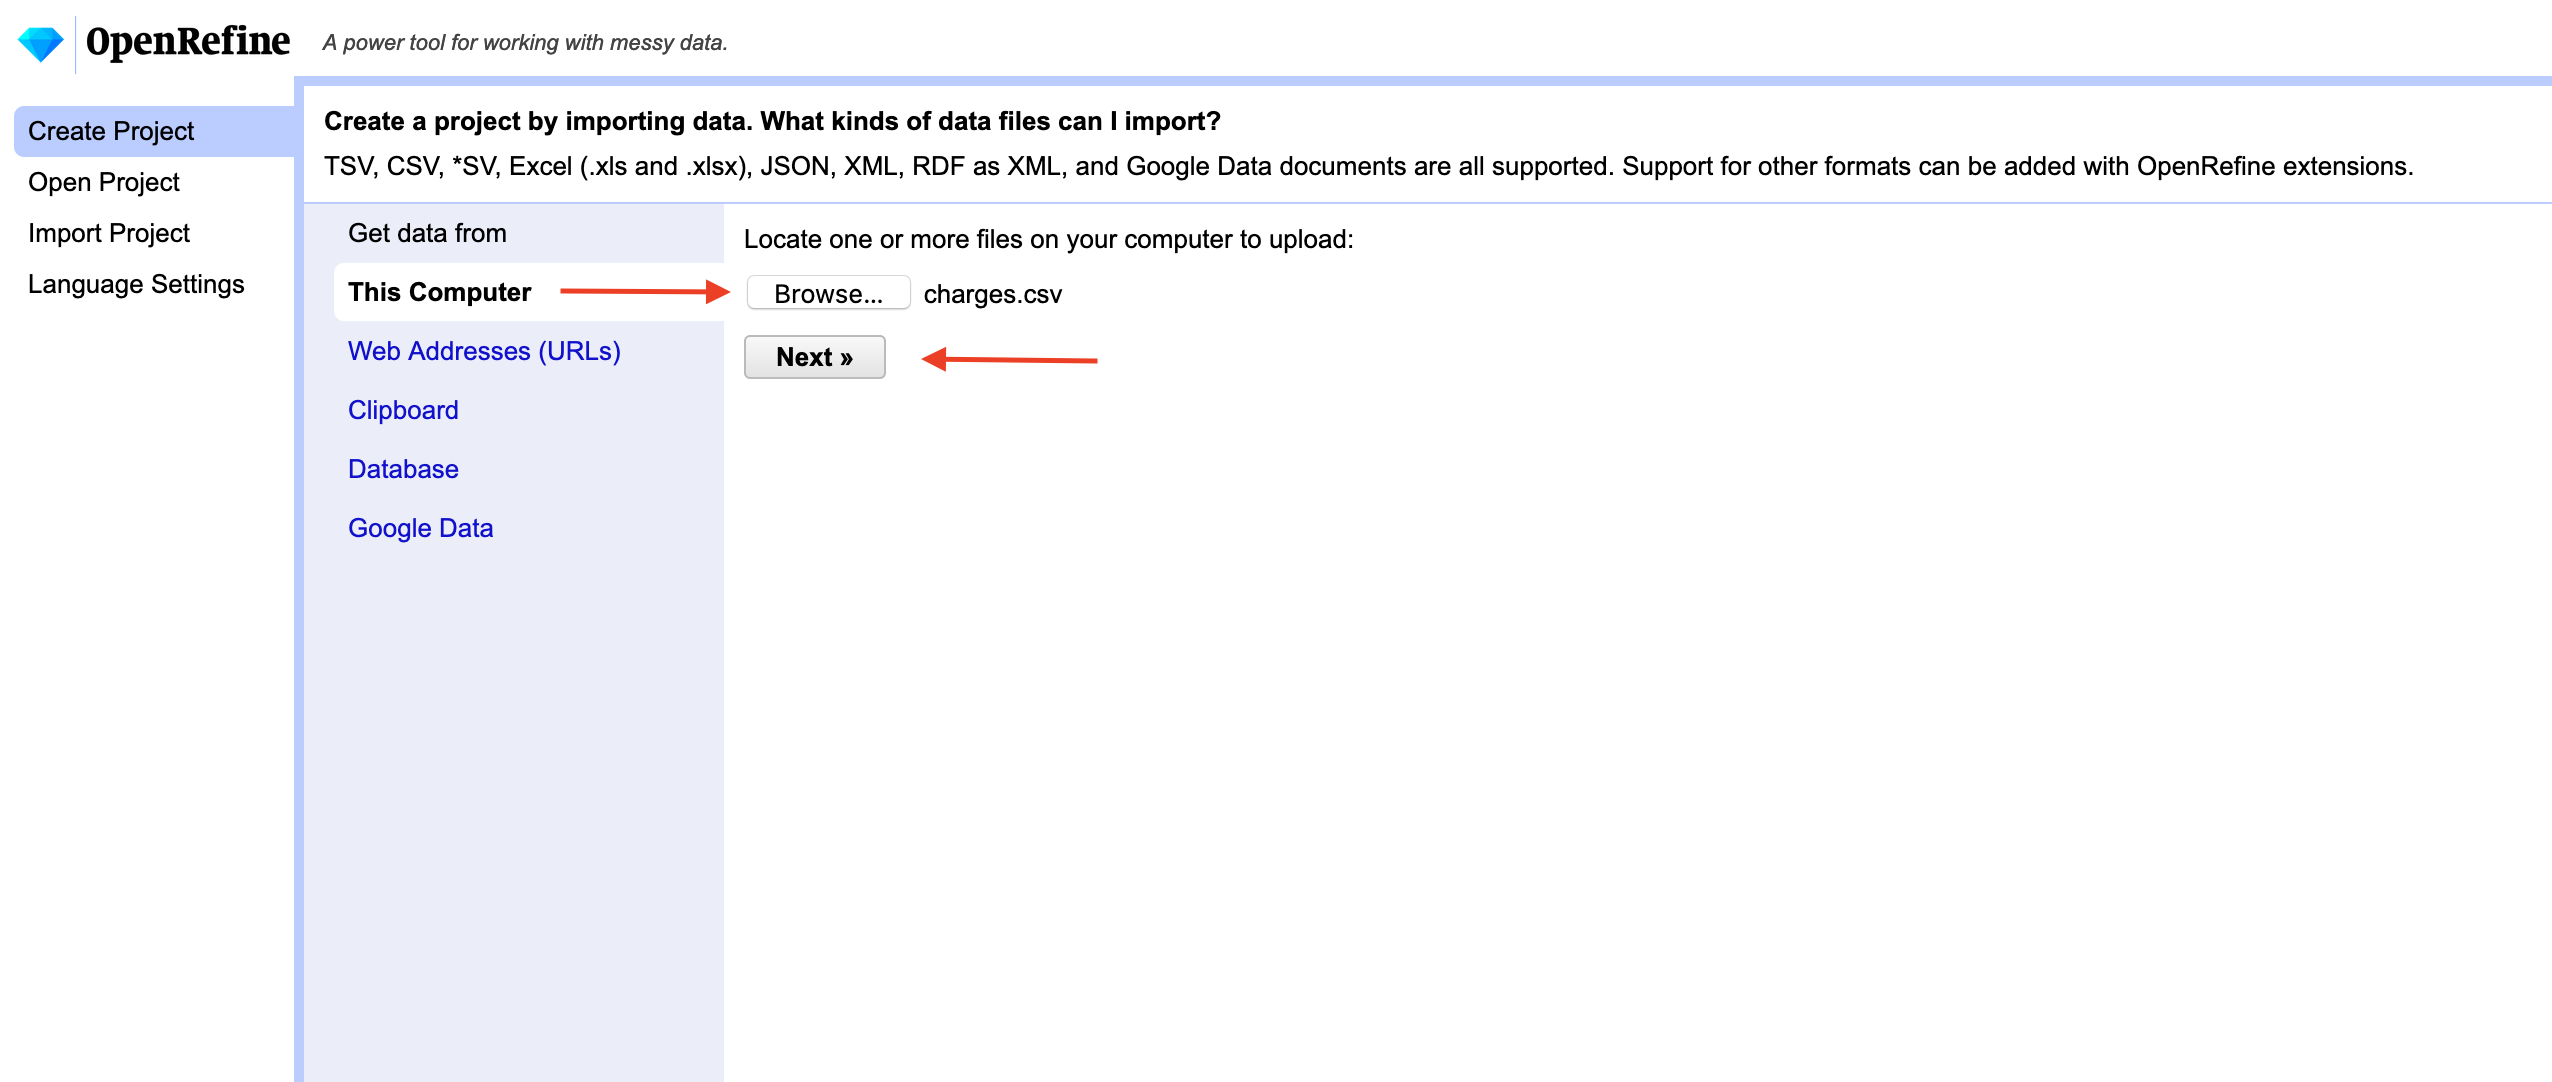
\includegraphics[width=35.44in]{images/open1}

After your data is loaded into the app, you'll get a screen to look over what the data looks like. On the top right corner, you'll see a button to create the project.

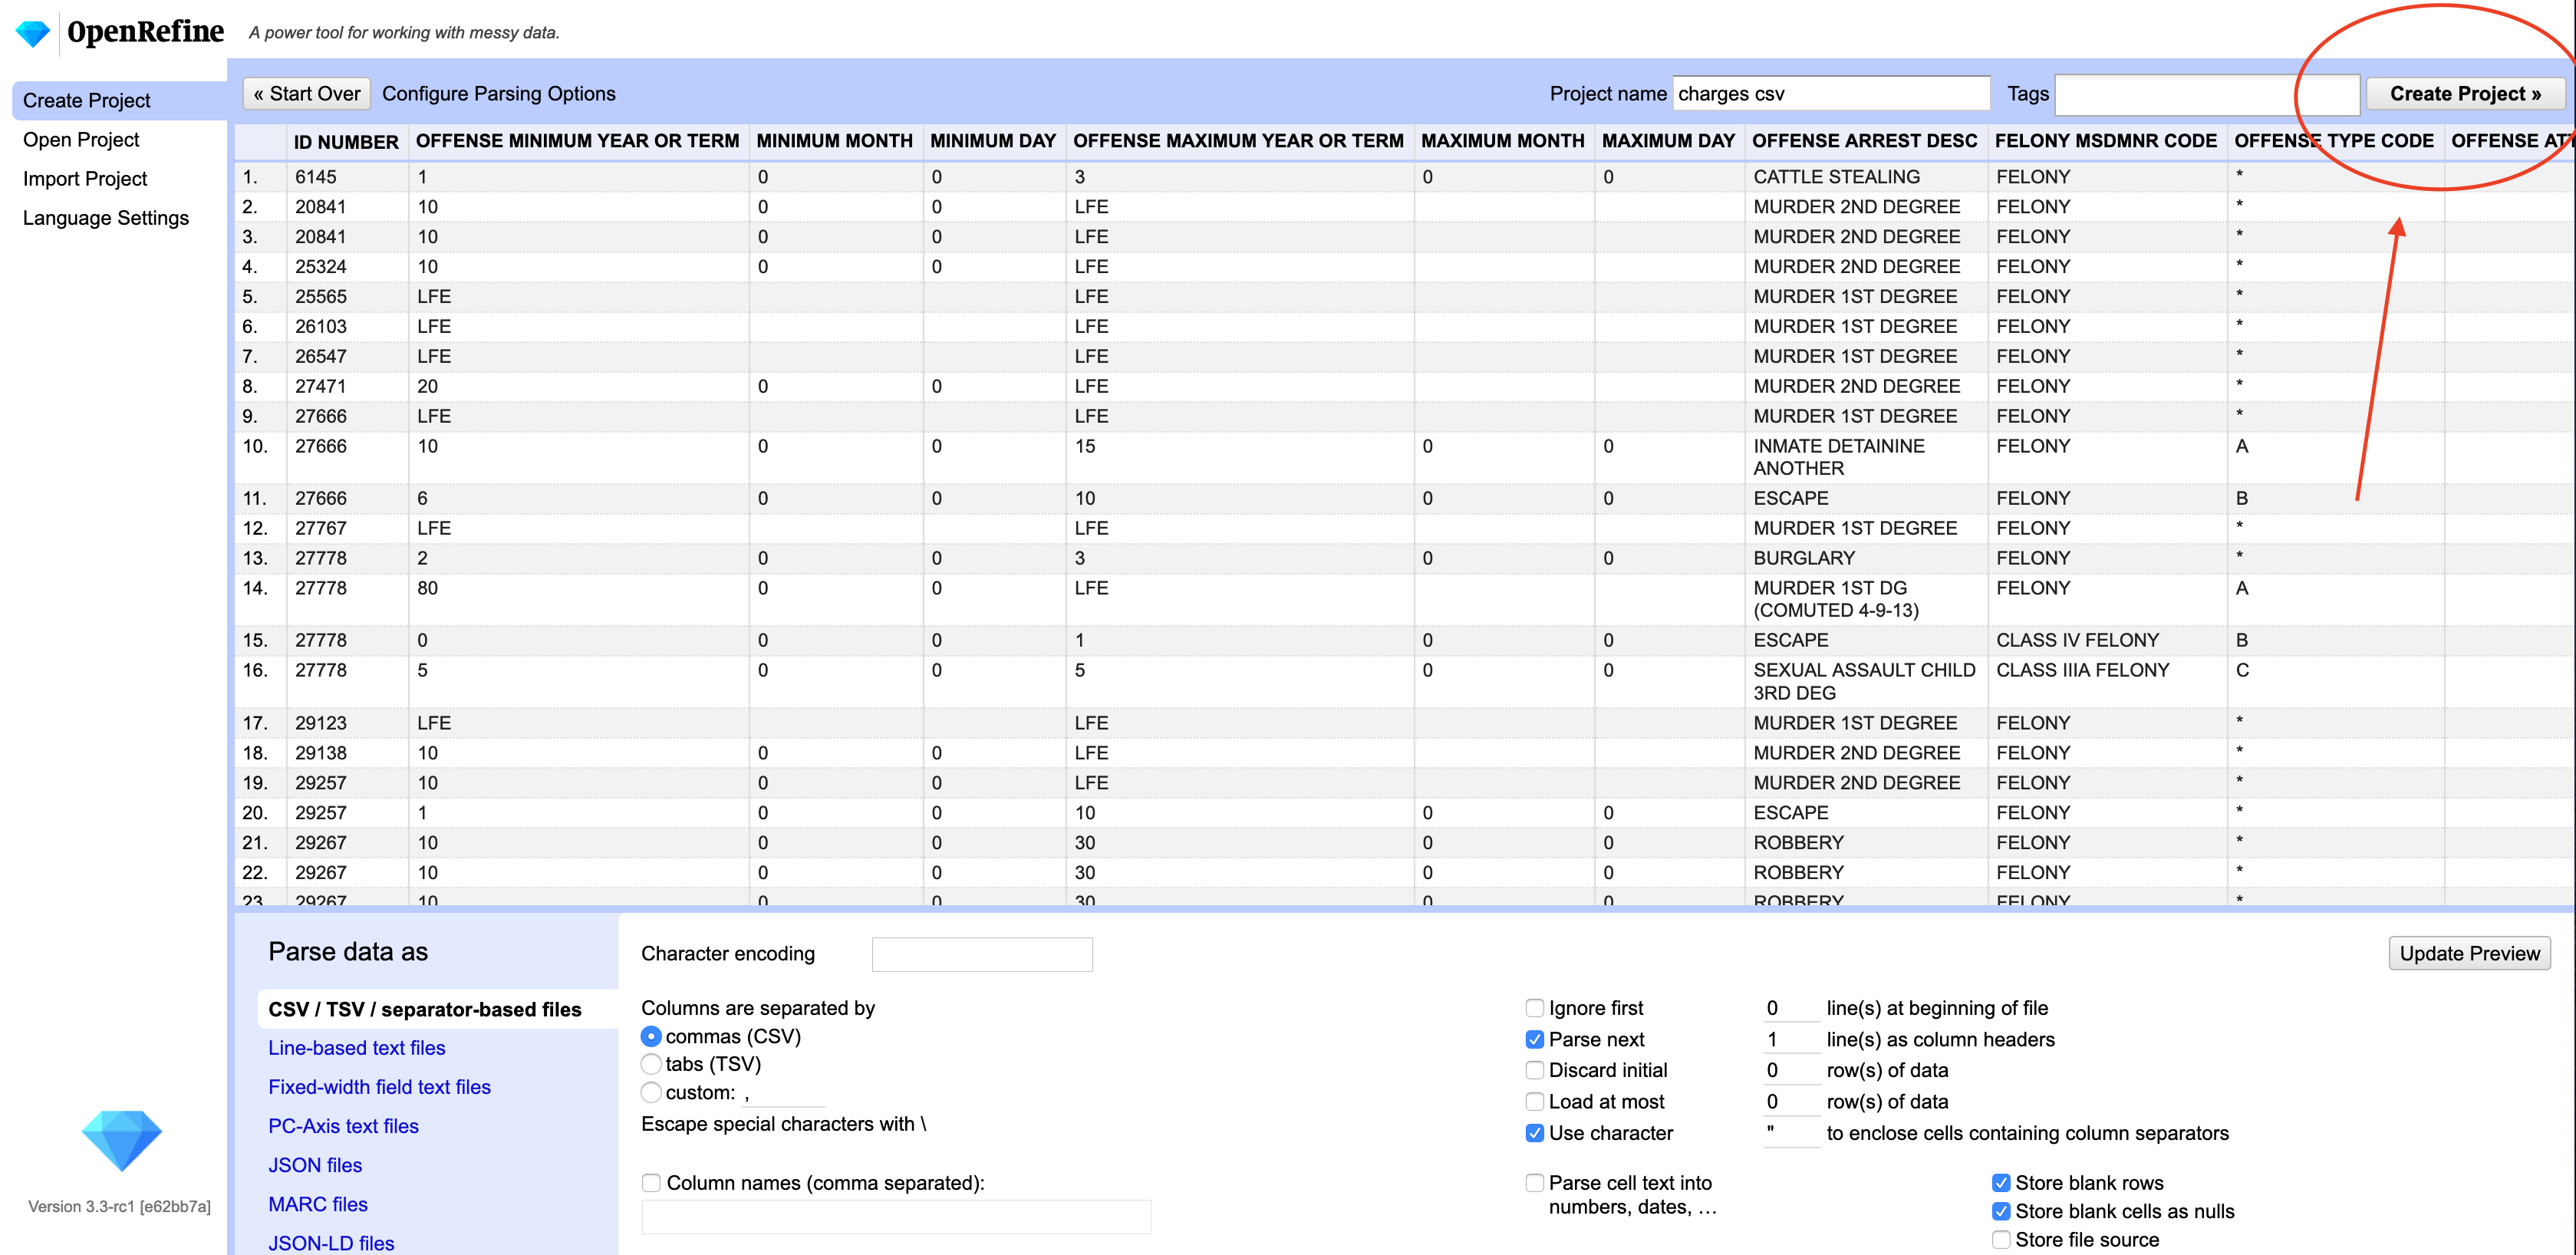
\includegraphics[width=46.64in]{images/open2}

The real power in Open Refine is in faceting. In our case, we're specifically going to use text faceting. Next to the OFFENSE ARREST DESC header, click the down arrow, then facet, then text facet.

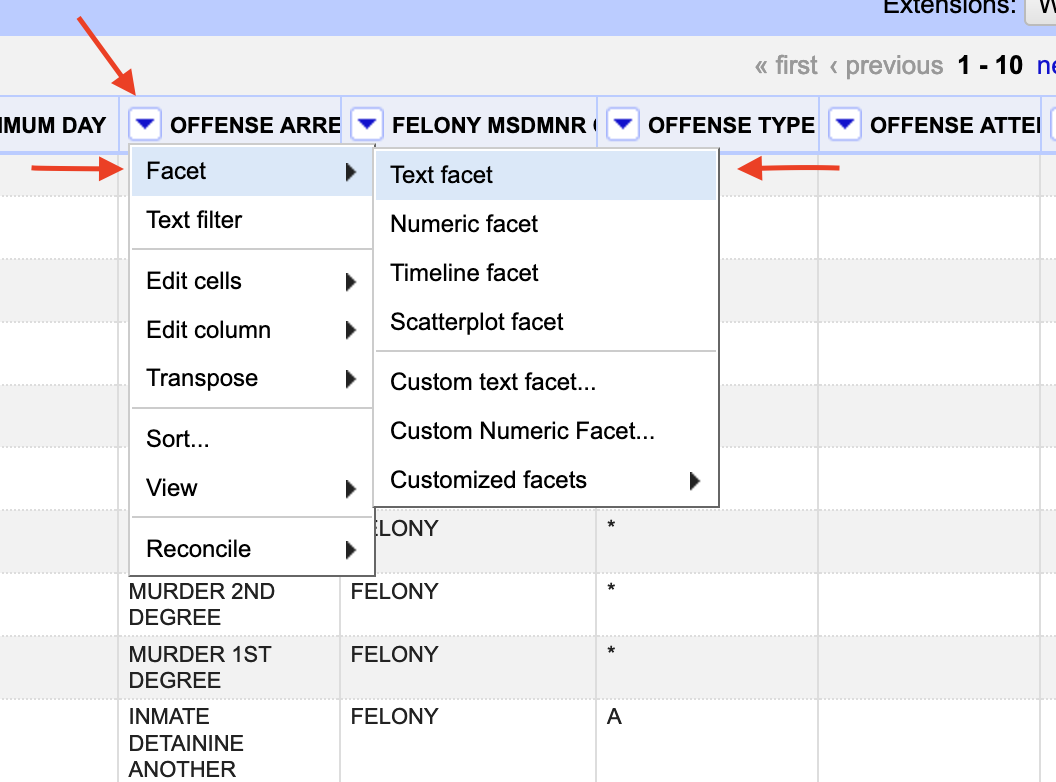
\includegraphics[width=14.67in]{images/open3}

After that, a new box will appear on the left. It tells us how many unique offenses are there: 4,082. And, there's a button on the right of the box that says Cluster. Click that.

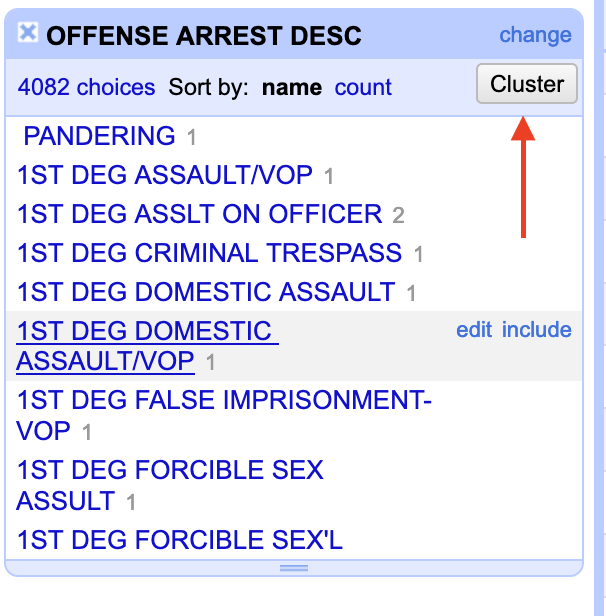
\includegraphics[width=8.42in]{images/open4}

The default clustering algorithm used is key collision, using the fingerprint function. This is the same method we used with Sheridan County above.

At the top, you'll see which method was used, and how many clusters that algorithm identified. Then, below that, you can see what those clusters are. Then, using human judgement, you can say if you agree with the cluster. If you do, click the merge checkbox. When it merges, the new result will be what it says in New Cell Value. Most often, that's the row with the most common result.

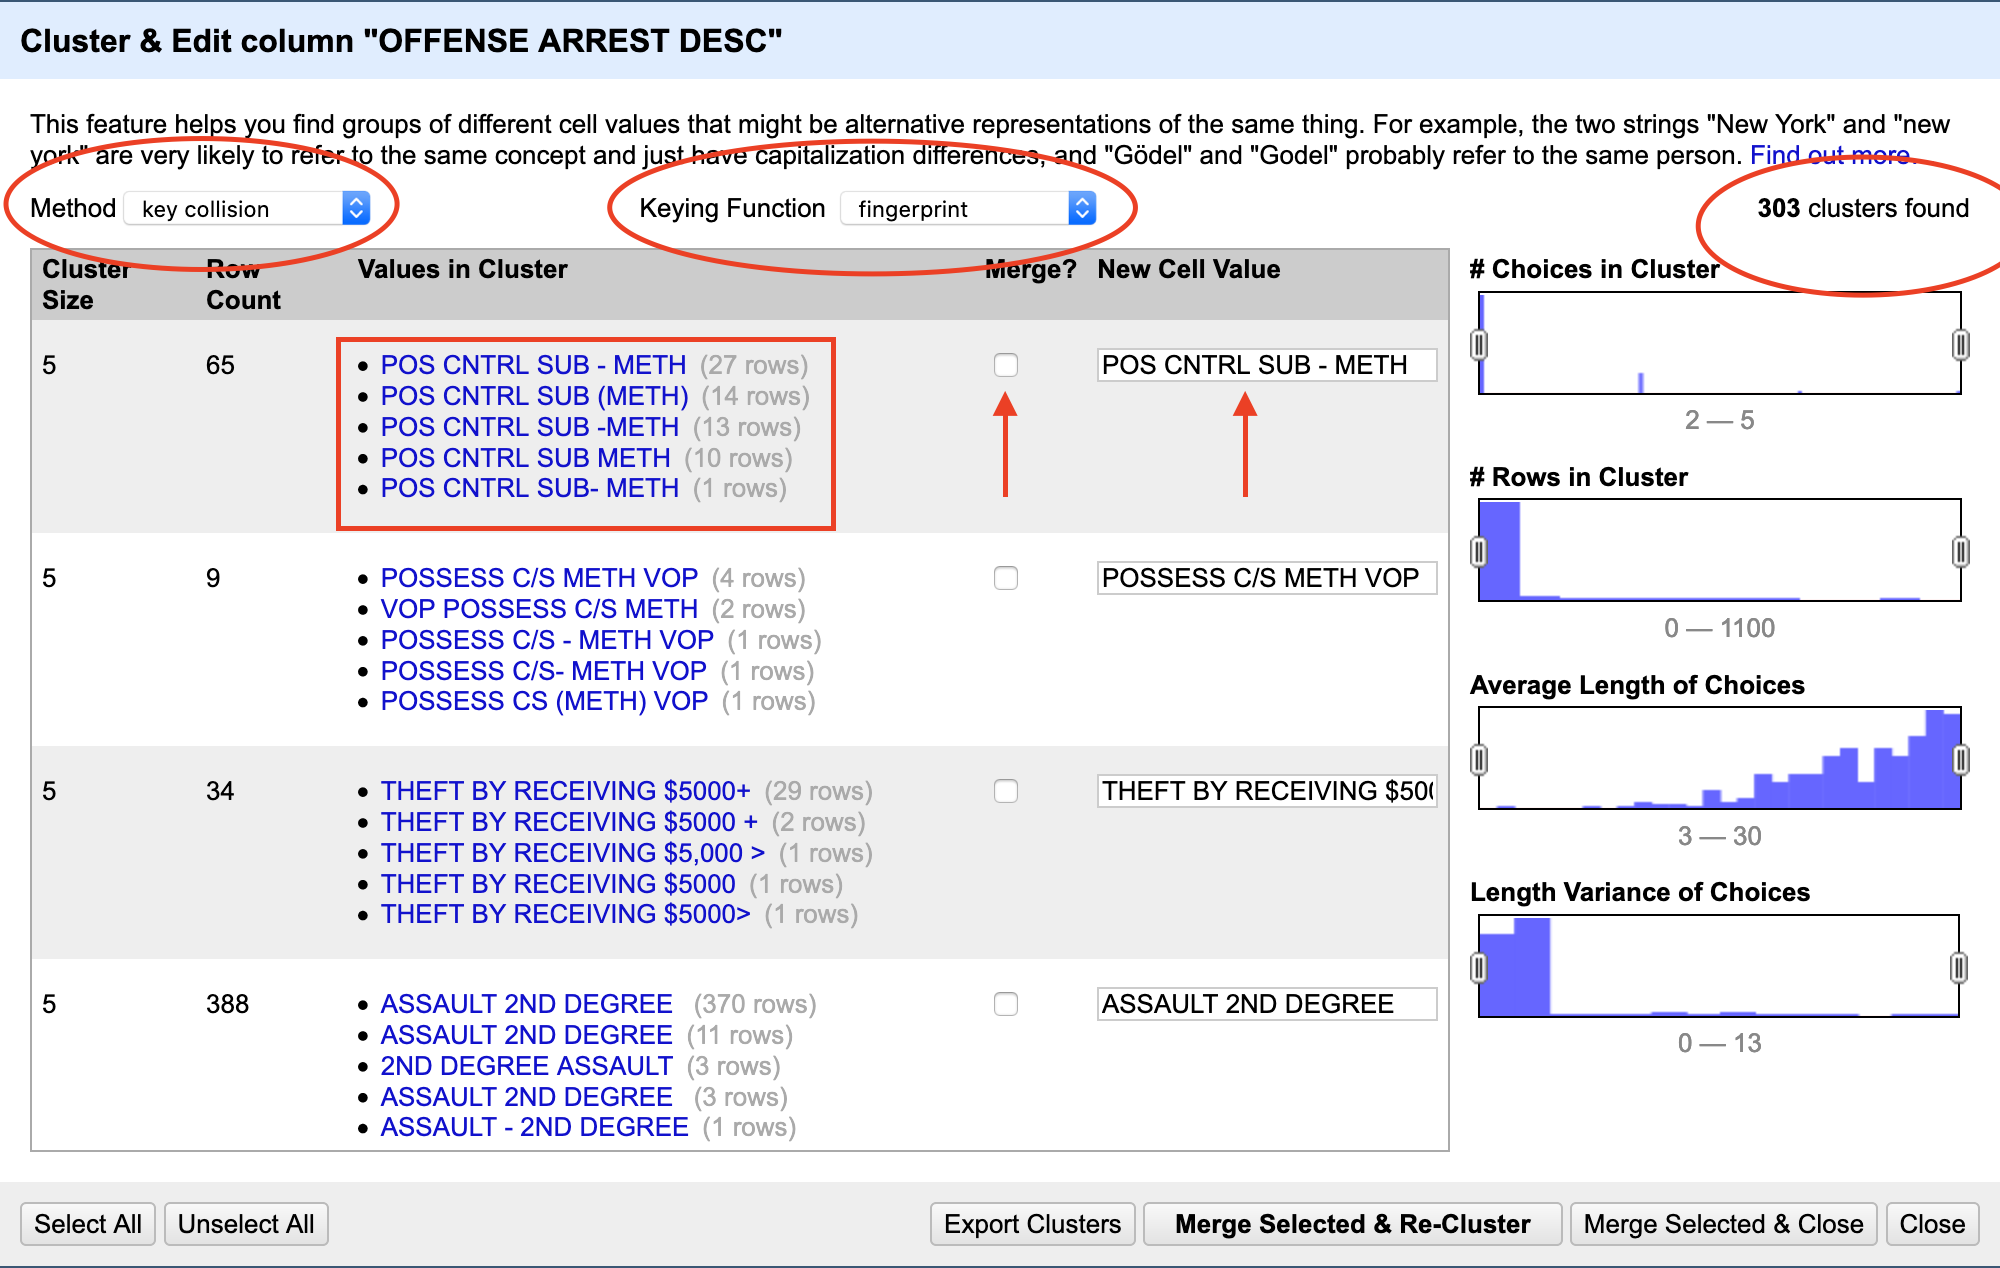
\includegraphics[width=27.78in]{images/open6}

Now begins the fun part: You have to look at all 303 clusters found and decide if they are indeed valid. The key collision method is very good, and very conservative. You'll find that most of them are usually valid.

When you're done, click Merge Selected and Re-Cluster.

If any new clusters come up, evaluate them. Repeat until either no clusters come up or the clusters that do come up are ones you reject.

Now. Try a new method. Rinse and repeat. You'll keep doing this, and if the dataset is reasonably clean, you'll find the end.

If it's not, it'll go on forever.

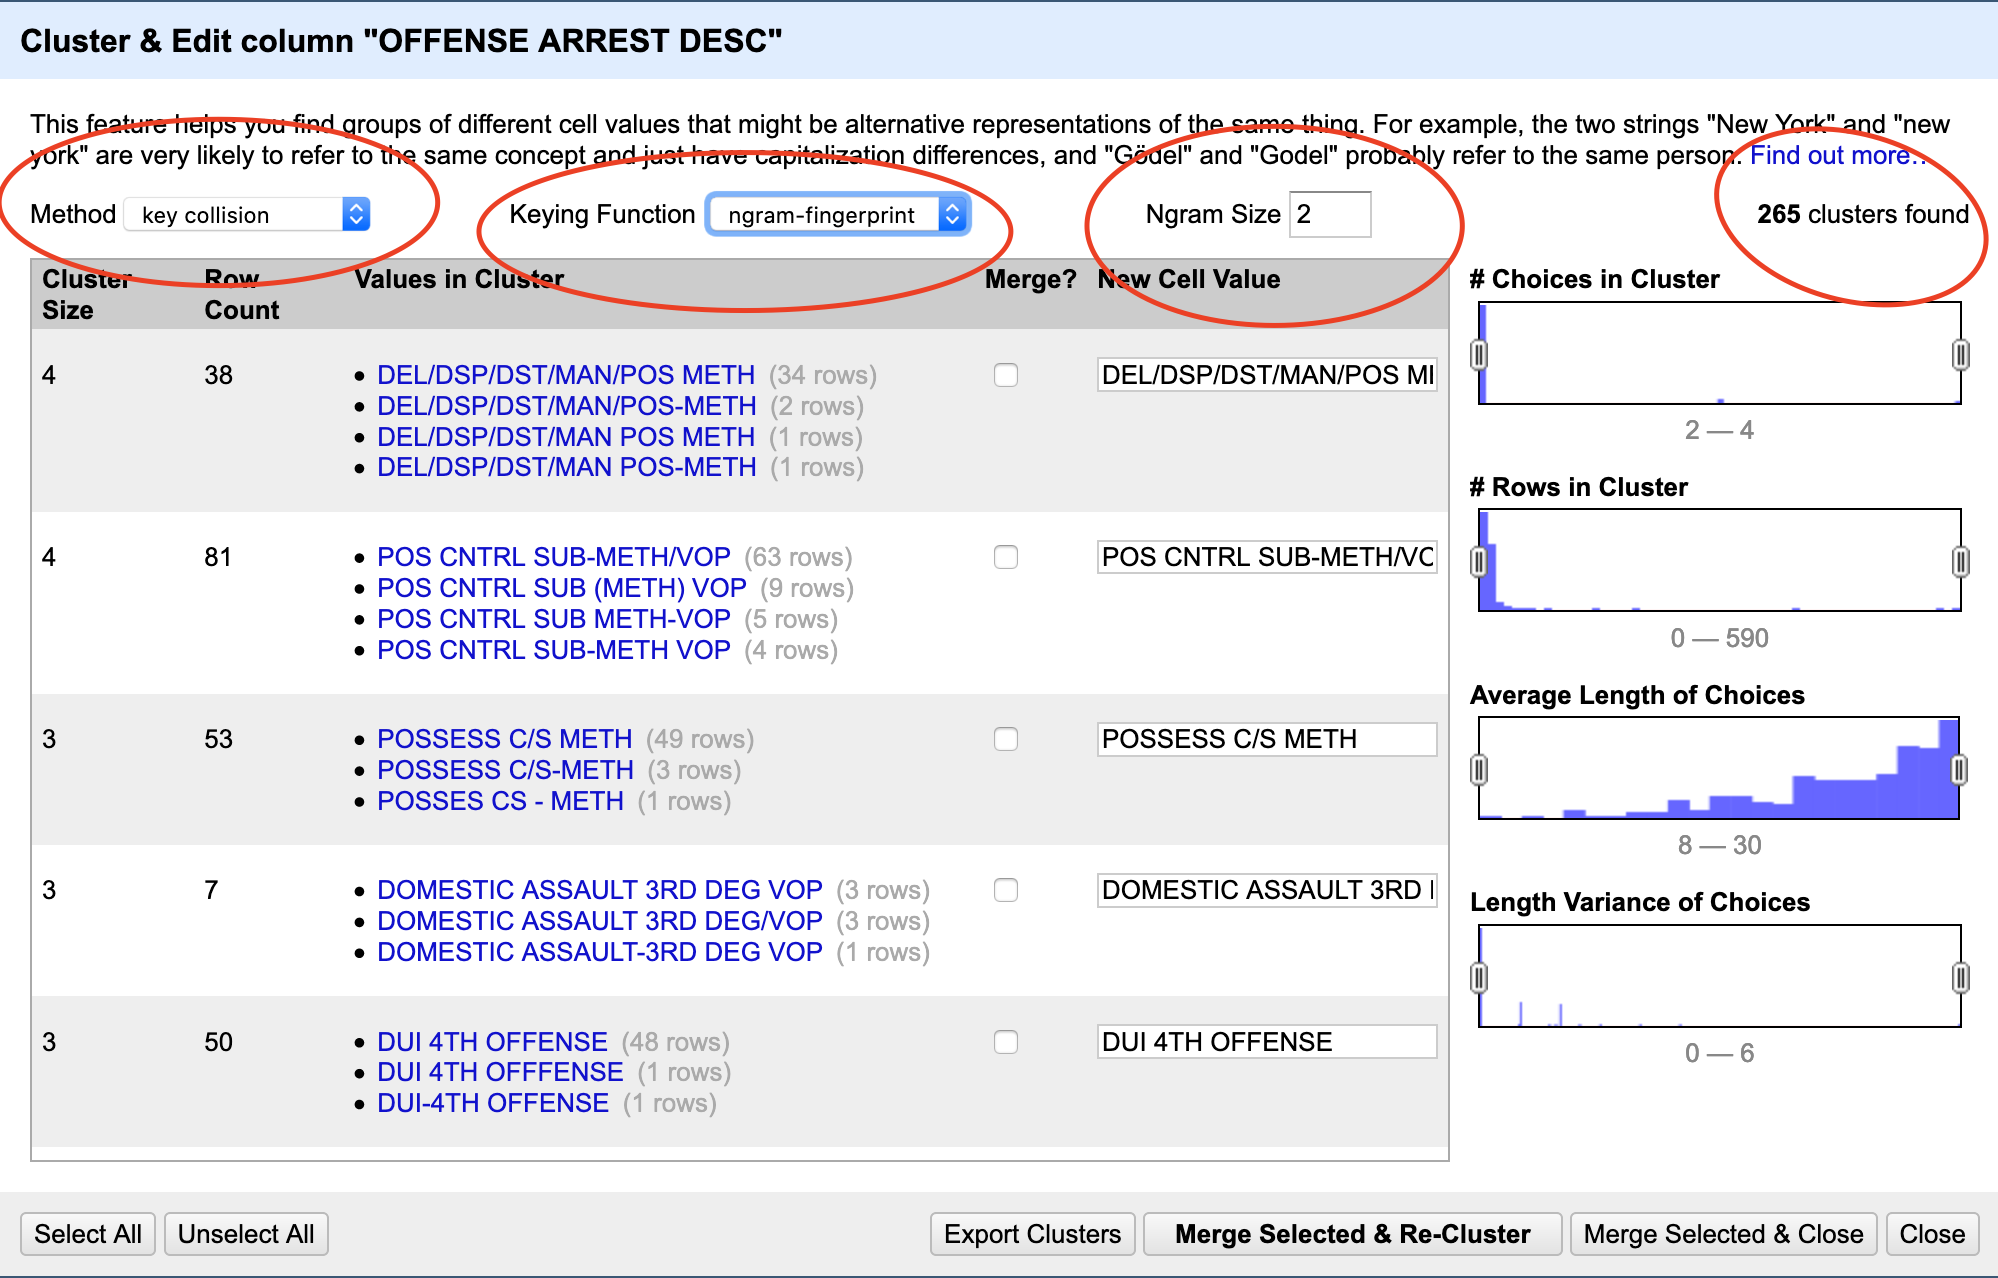
\includegraphics[width=27.75in]{images/open7}

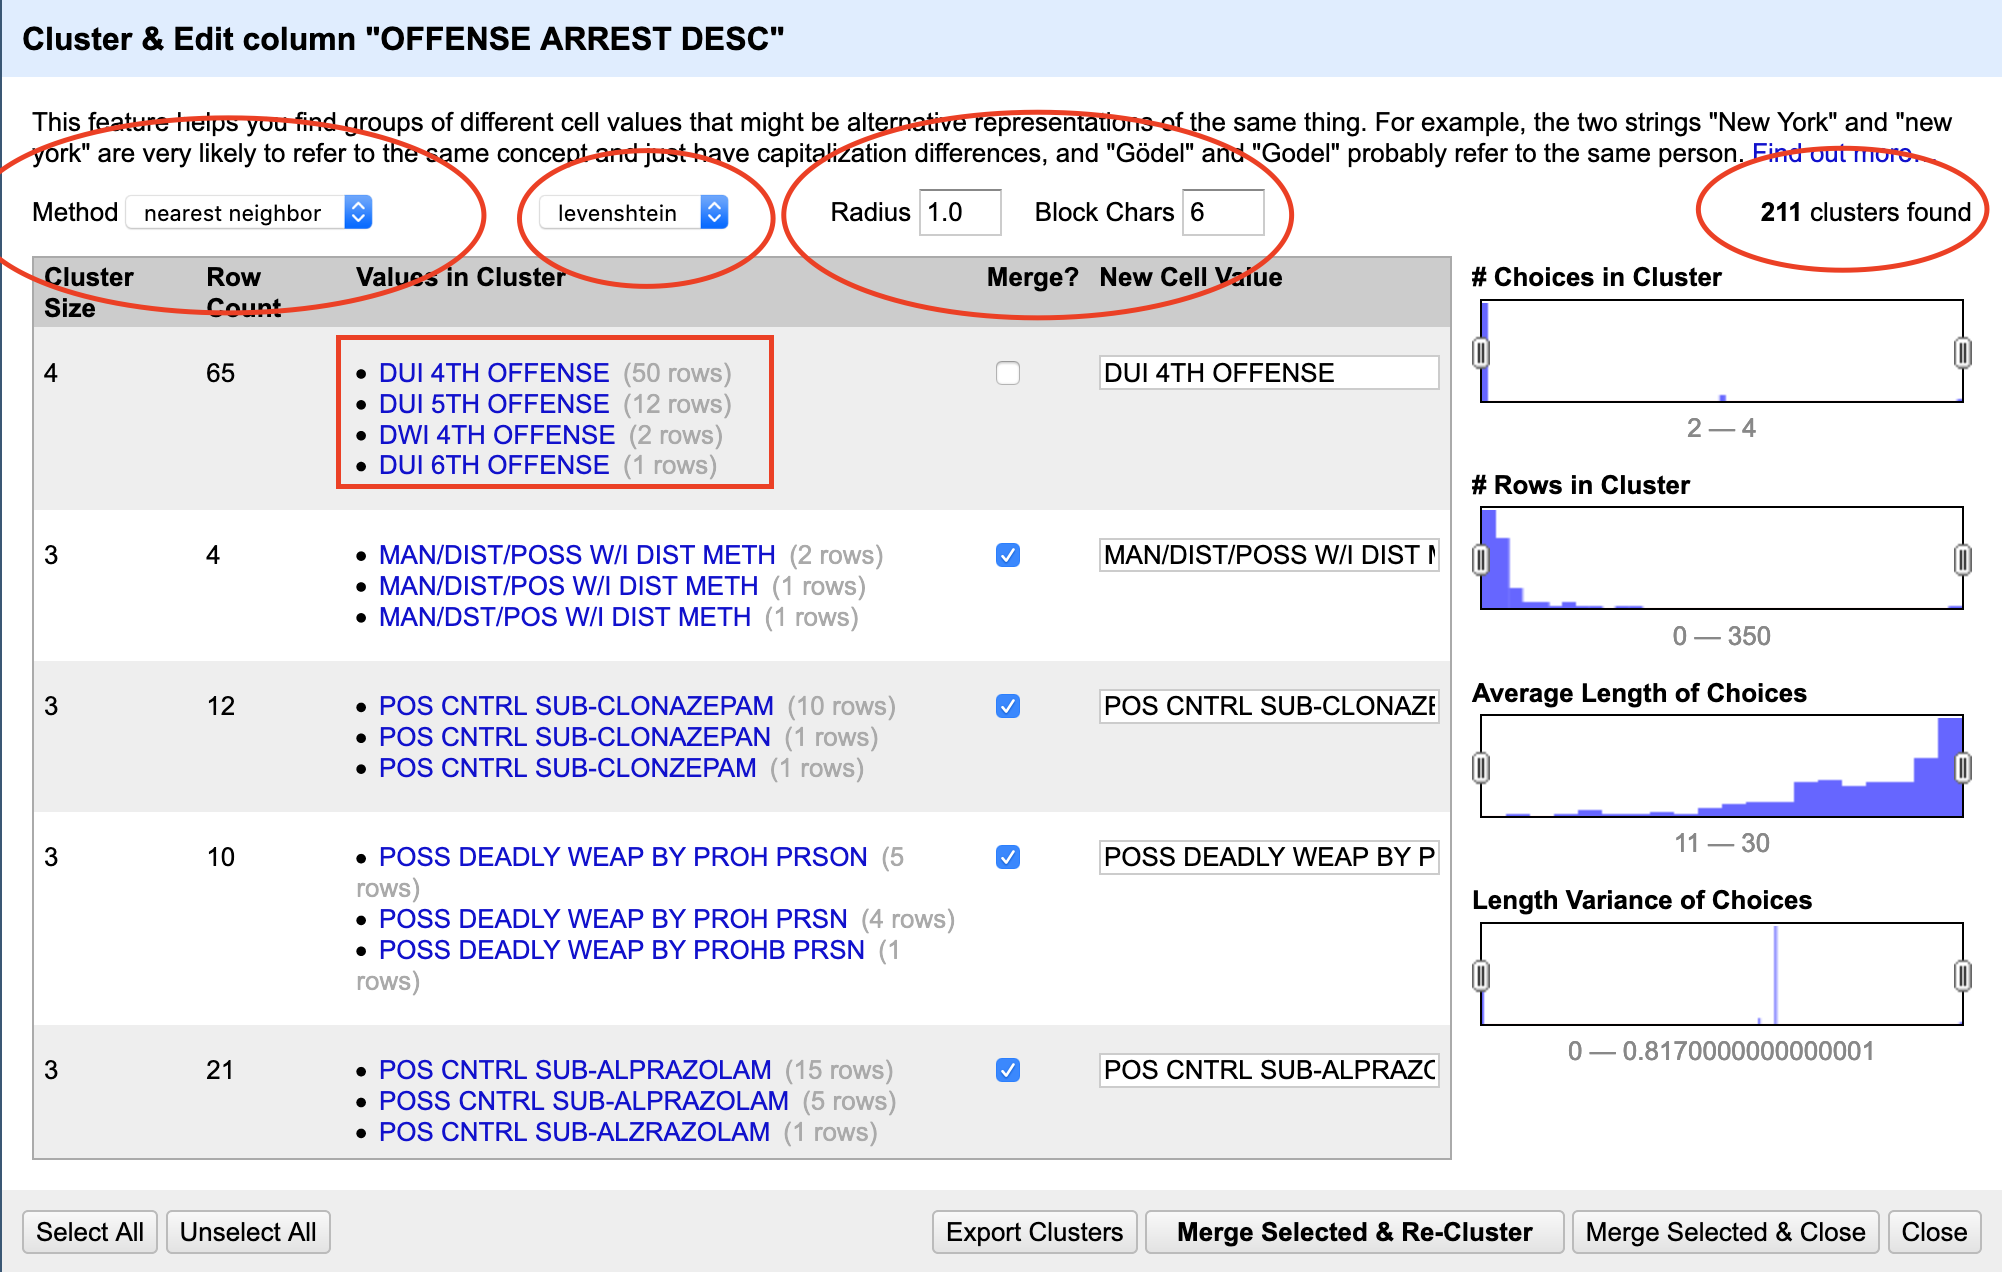
\includegraphics[width=27.81in]{images/open8}

A question for all data analysts -- if the dataset is bad enough, can it ever be cleaned?

There's no good answer. You have to find it yourself.

\hypertarget{cleaning-data-part-iv-pdfs}{%
\chapter{Cleaning Data Part IV: PDFs}\label{cleaning-data-part-iv-pdfs}}

The next circle of Hell on the Dante's Inferno of Data Journalism is the PDF. Governments everywhere love the PDF and publish all kinds of records in a PDF. The problem is a PDF isn't a data format -- it's a middle finger, saying I've Got Your Accountability Right Here, Pal.

It's so ridiculous that there's a constellation of tools that do nothing more than try to harvest tables out of PDFs. There are online services like \href{https://www.cometdocs.com/}{CometDocs} where you can upload your PDF and point and click your way into an Excel file. There are mobile device apps that take a picture of a table and convert it into a spreadsheet. But one of the best is a tool called \href{https://tabula.technology/}{Tabula}. It was build by journalists for journalists.

There is a version of Tabula that will run inside of R -- a library called Tabulizer -- but the truth is I'm having the hardest time installing it on my machine, which leads me to believe that trying to install it across a classroom of various machines would be disasterous. The standalone version works just fine.

Unfortunately, harvesting tables from PDFs with Tabula is an exercise in getting your hopes up, only to have them dashed. We'll start with an example.

\hypertarget{when-it-looks-good-but-goes-wrong}{%
\section{When it looks good, but goes wrong}\label{when-it-looks-good-but-goes-wrong}}

Every year, the University of Nebraska-Lincoln publishes dozens of PDFs that give you interesting demographic information about students, the faculty and a variety of other things. But all of it -- every little bit of it -- is in a PDF. And most of them are designed to look ``nice'' not convey data. Even when they do very obviously look like they came from a spreadsheet -- like someone printed the spreadsheet to a PDF so they could put it on the web -- it doesn't work.

A perfect example of this is the data showing the \href{https://iea.unl.edu/dmdocuments/050_fall_2018_enrl_p100.pdf}{breakdown of students by degree, major, race and sex}. Open it up, it looks like a spreadsheet but in a PDF.

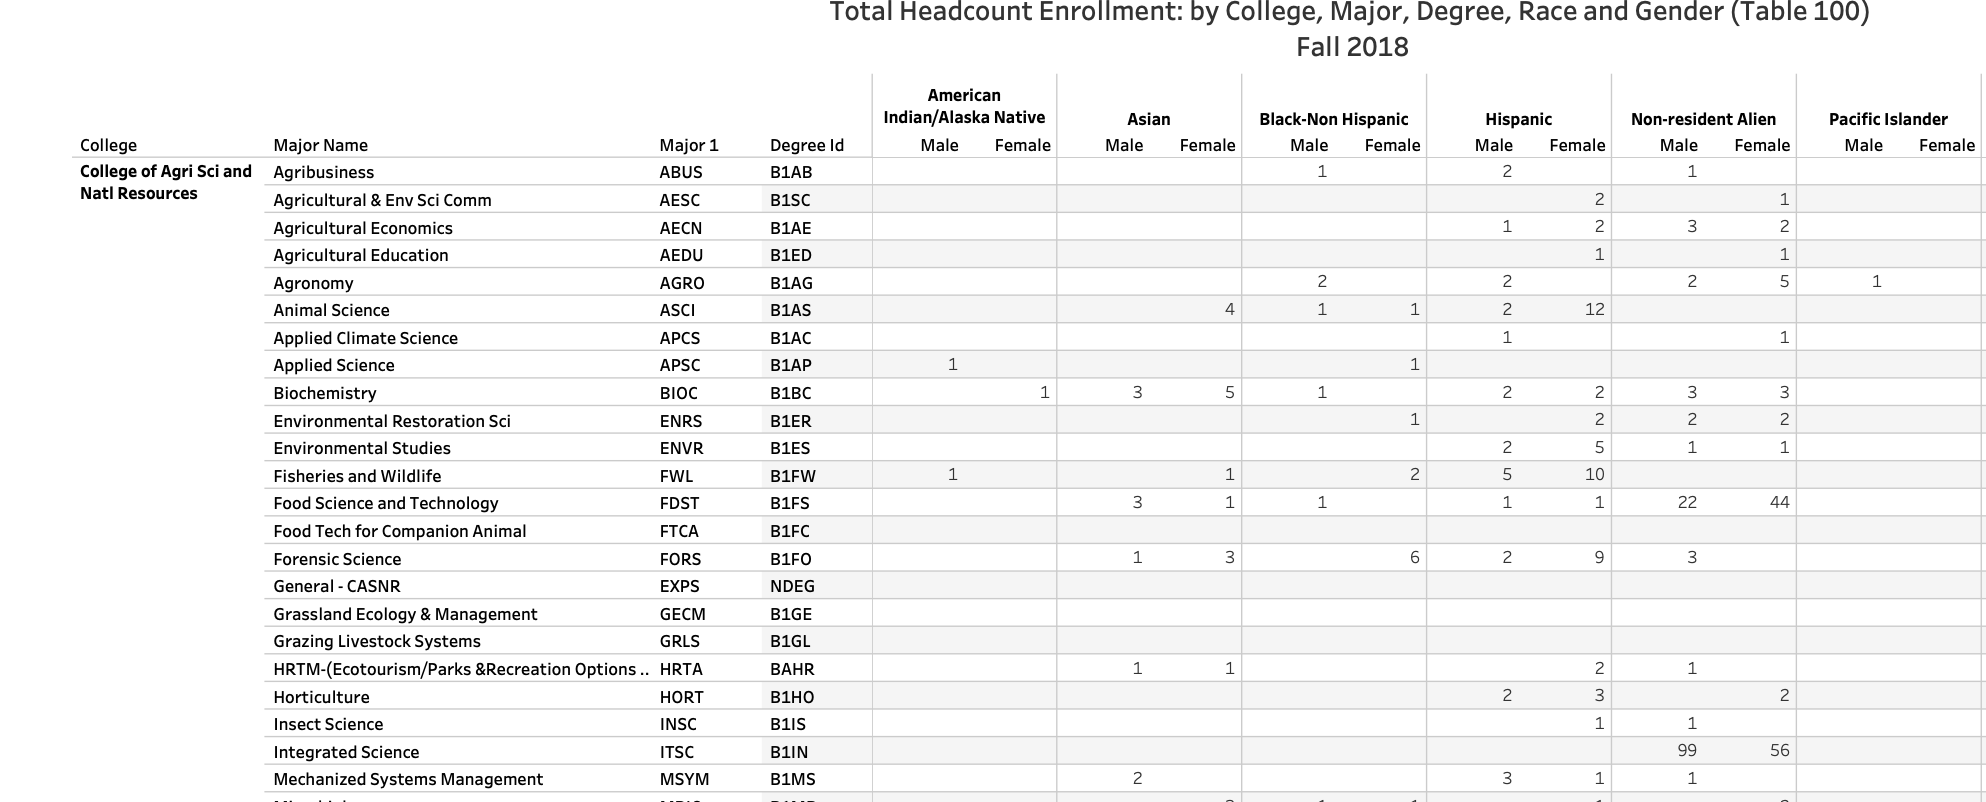
\includegraphics[width=27.58in]{images/pdfs1}

\href{https://tabula.technology/}{Download and install Tabula}. Tabula works much the same way as Open Refine does -- it works in the browser by spinning up a small webserver in
your computer.

When Tabula opens, you click browse to find the PDF on your computer somewhere, and then click import.

After it imports, click autodetect tables. You'll see red boxes appear around what Tabula believes are the tables. You'll see it does a pretty good job at this.

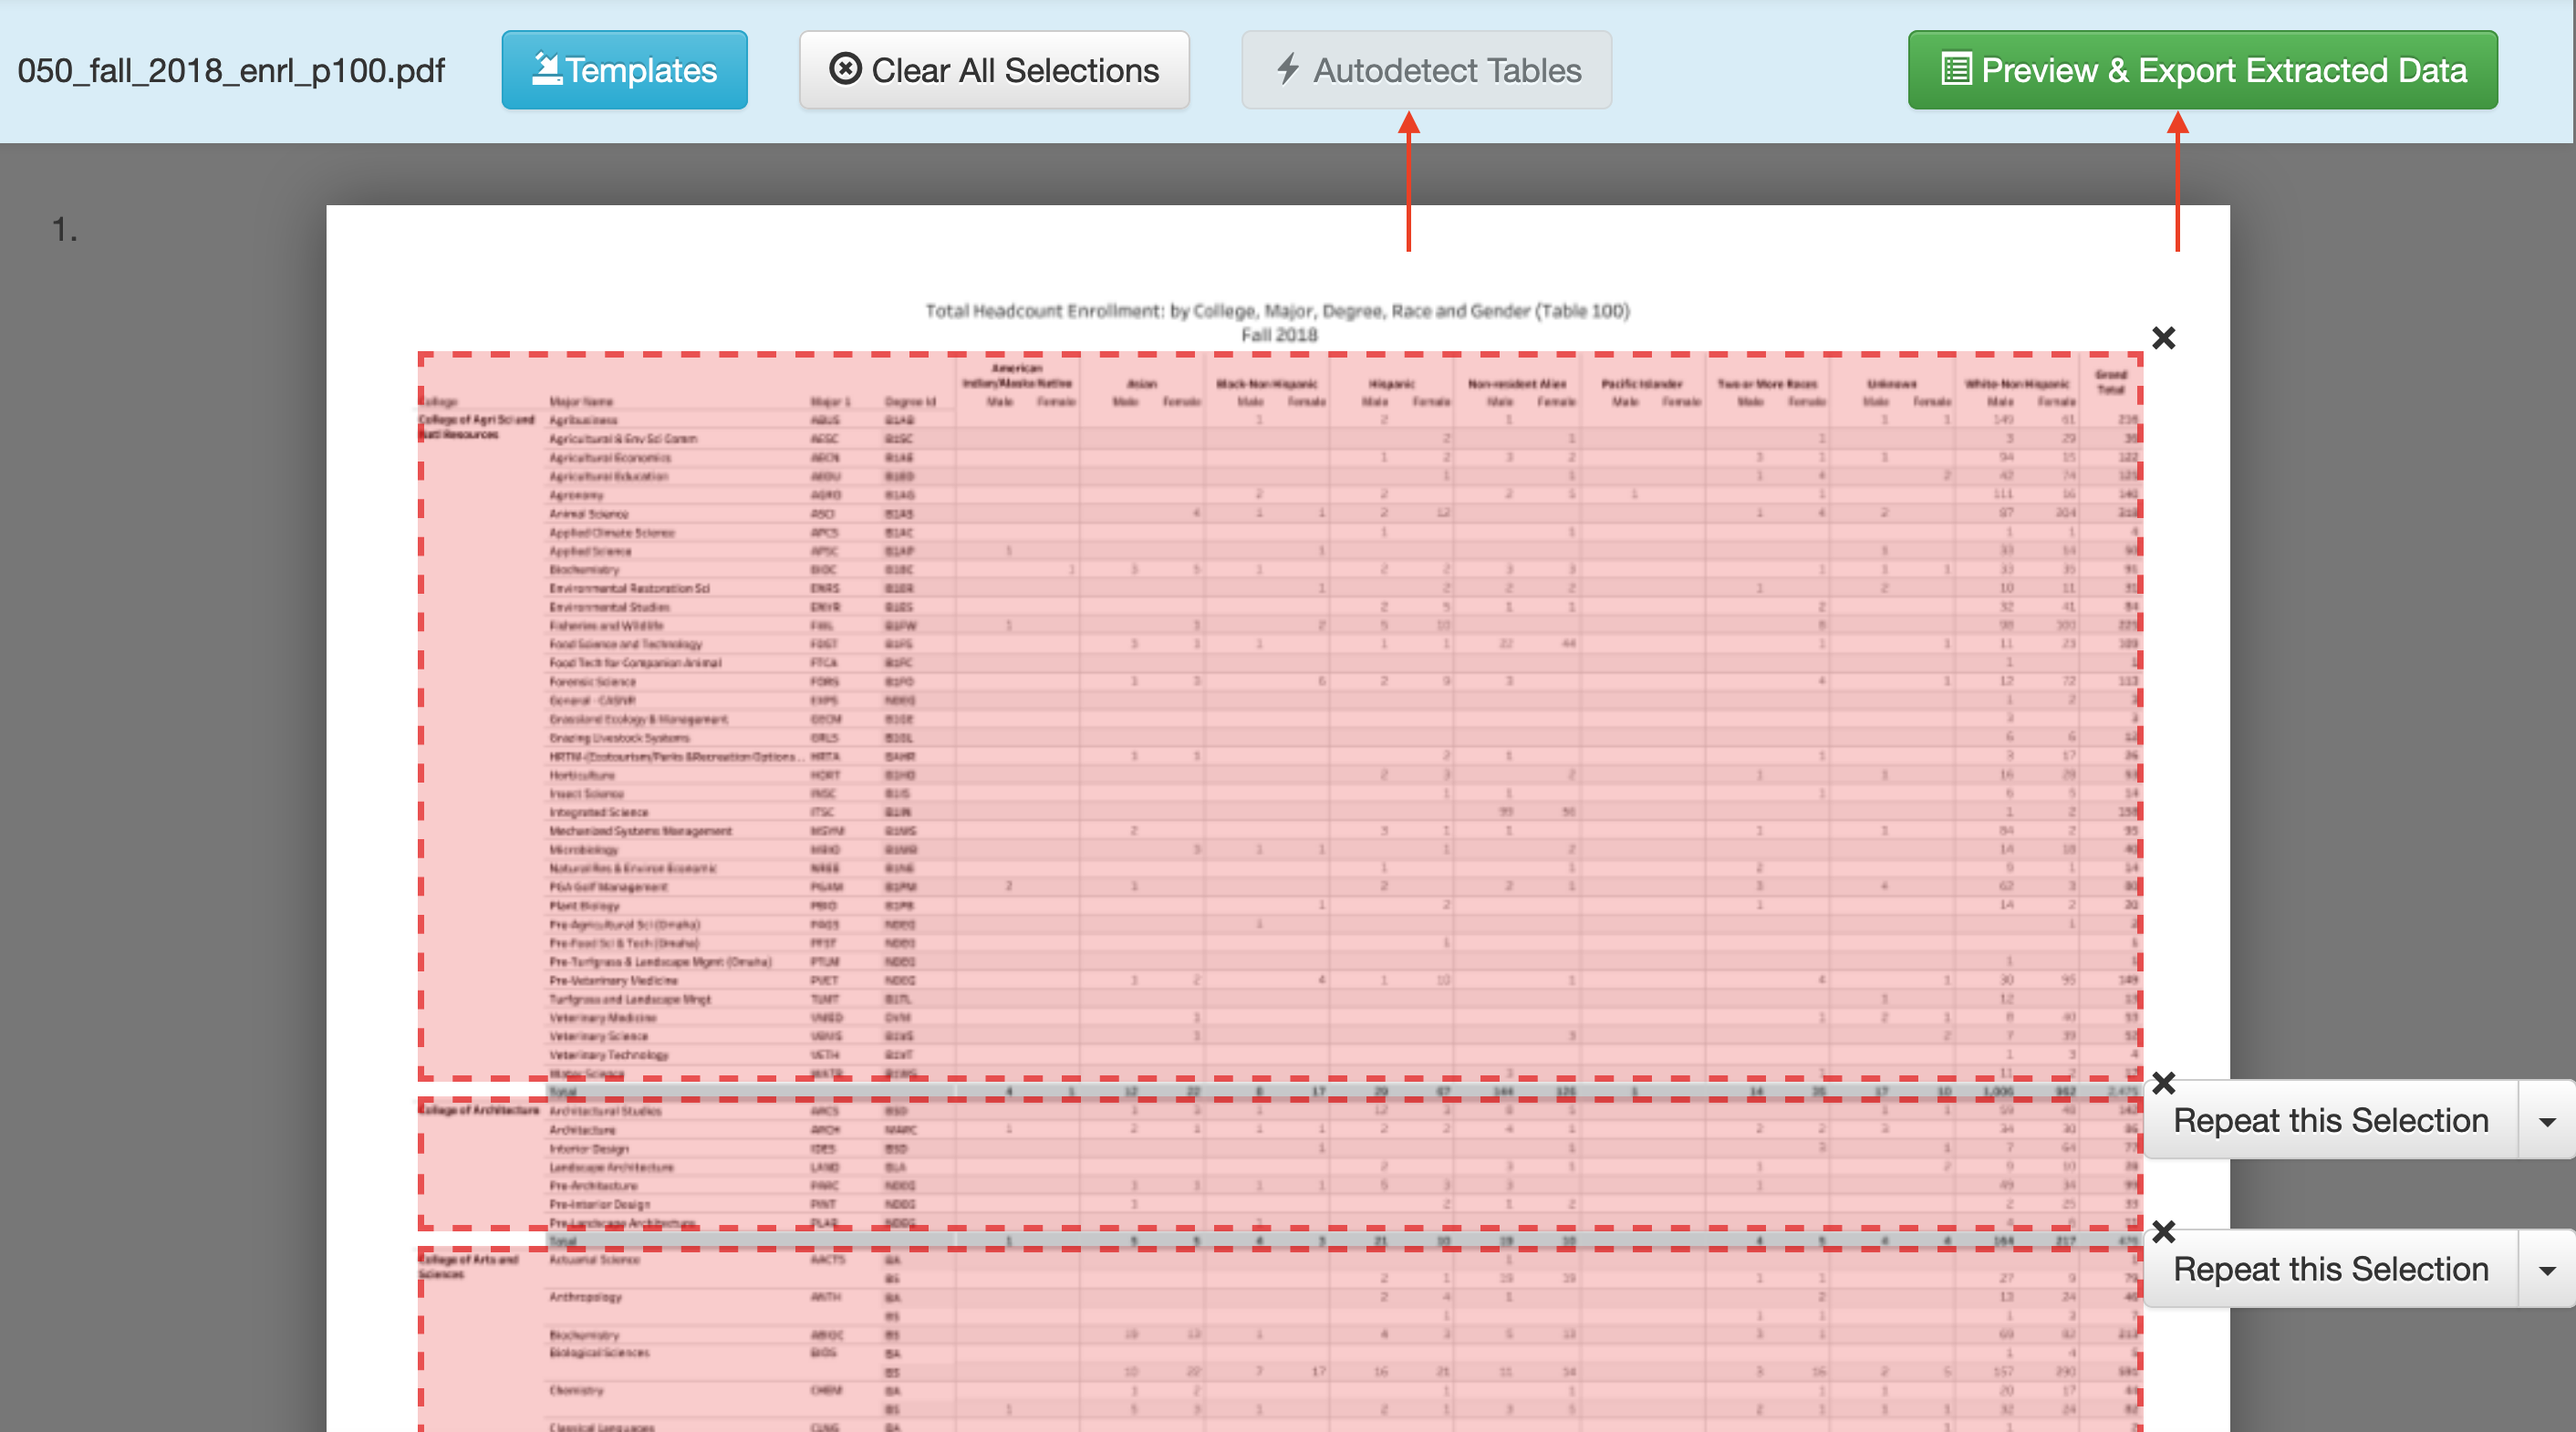
\includegraphics[width=39.22in]{images/pdfs2}

If you like what you see, click Preview and Export Extracted Data.

And here's where it all starts to go wrong.

You'll see at first it looks good -- you get a reasonable representation of the table. But look at the first line.

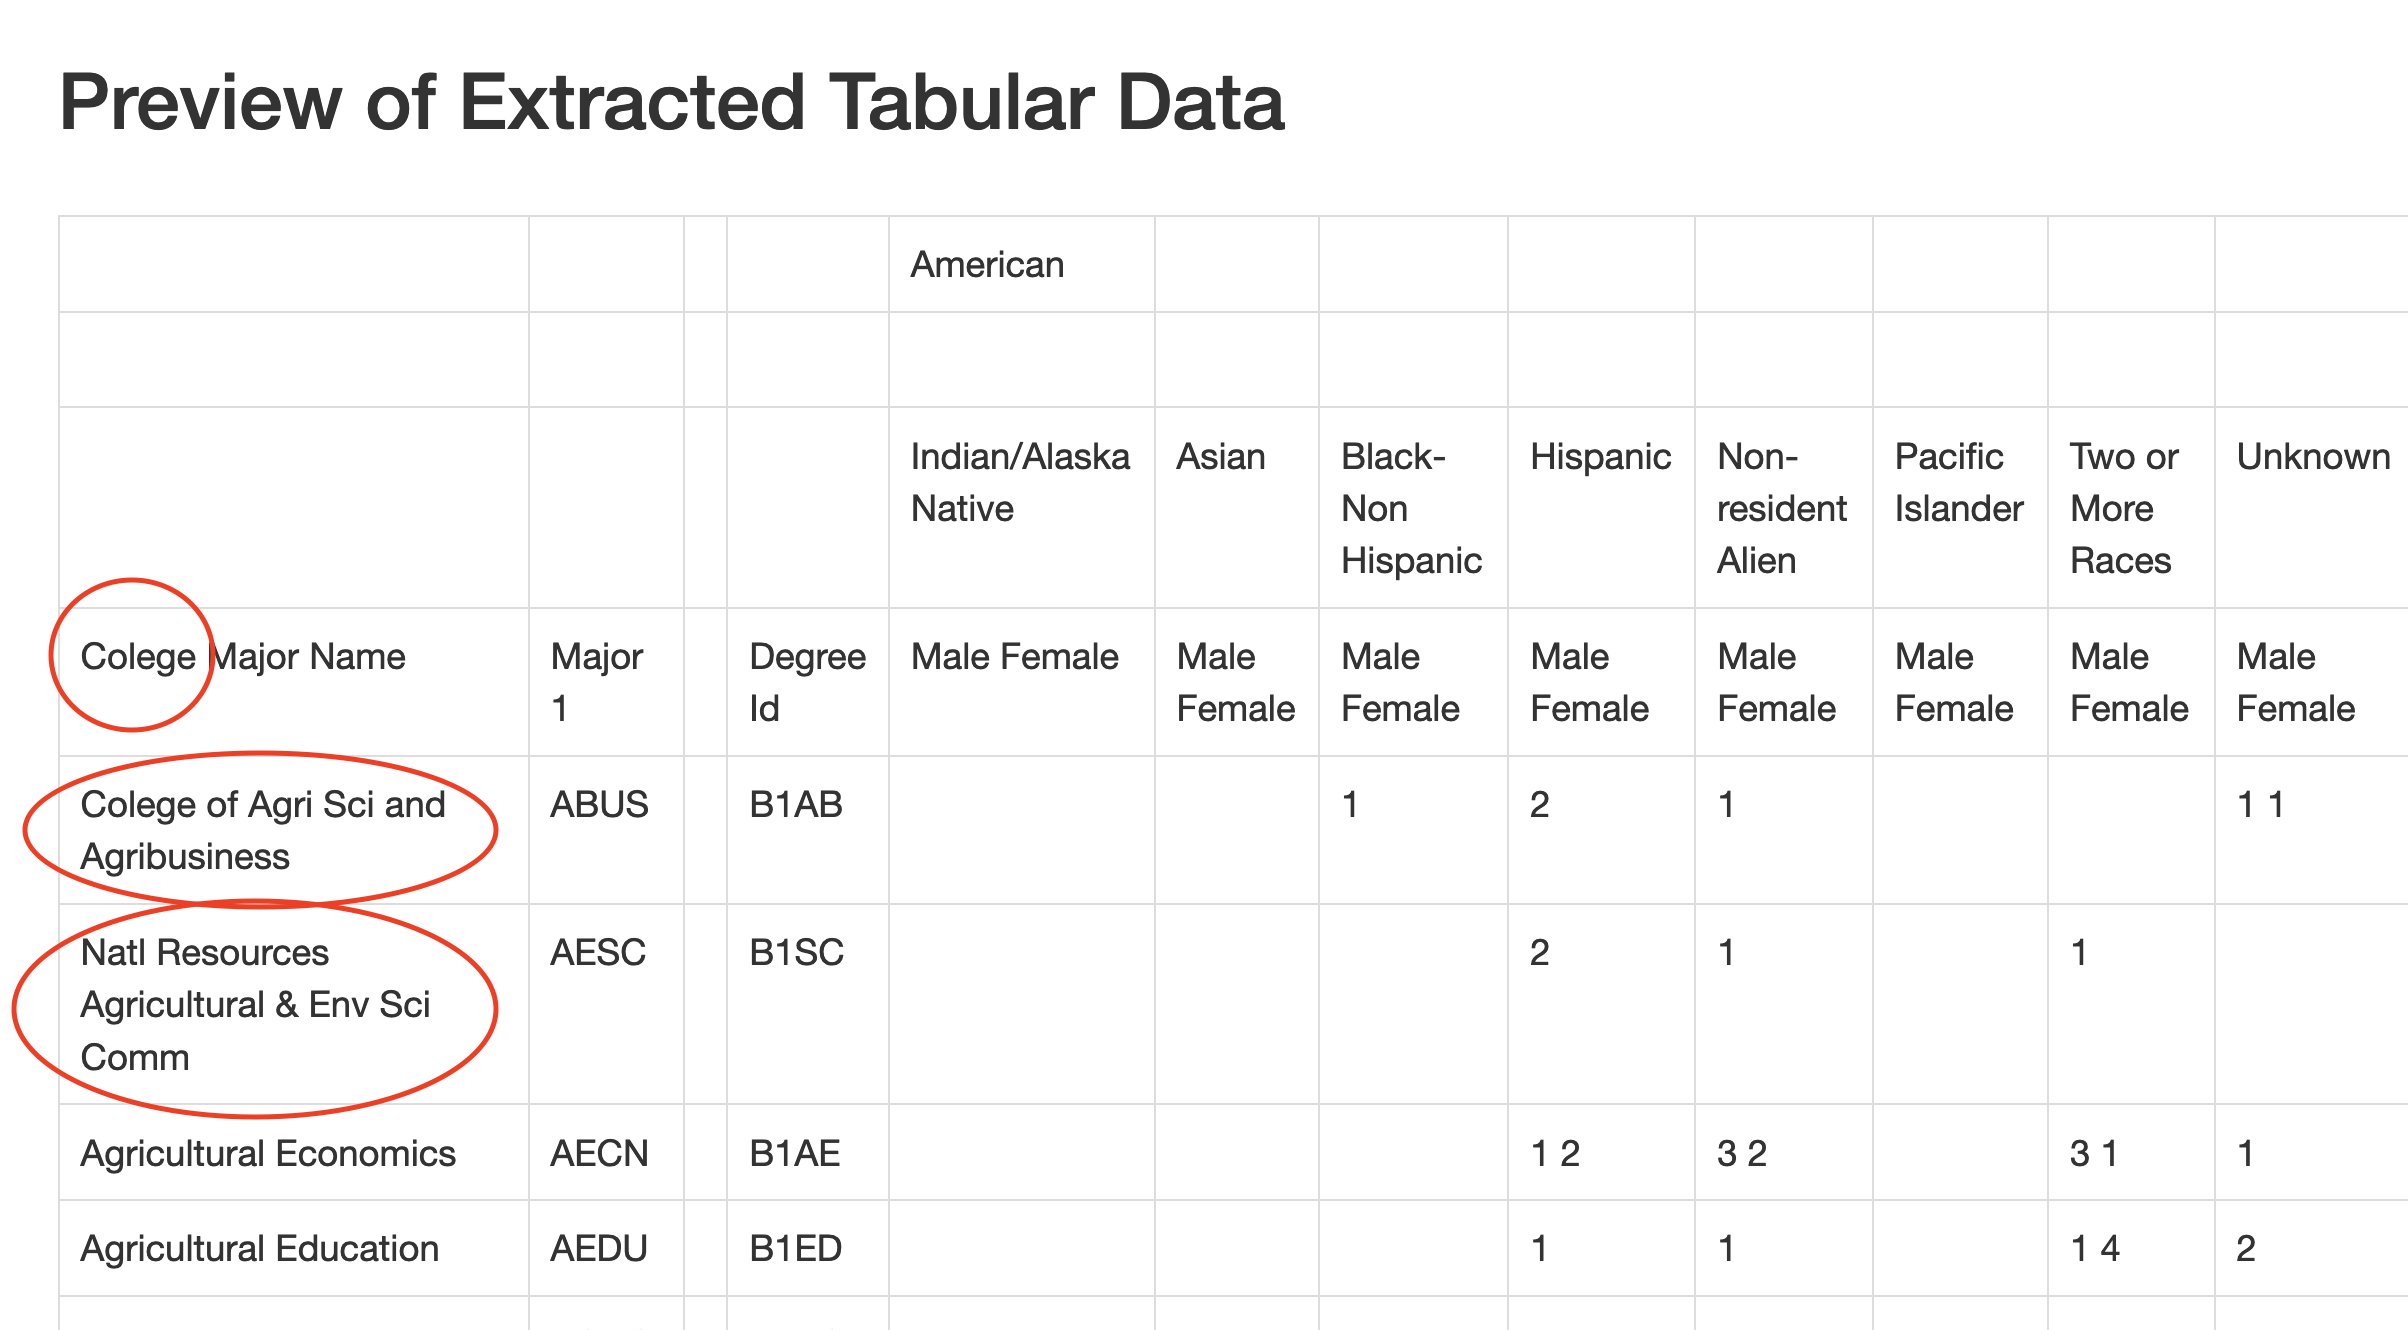
\includegraphics[width=33.44in]{images/pdfs3}

First, the misspelling of college is disturbing. Did a university document misspell it? No.~Which means Tabula is reading two ls as one. That's \ldots{} not good.

Second, notice how the College of Agri Sci and Natl Resources, which was in it's own column before have been merged, somewhat inartfully, into the first column of major names. There is no major Colege of Agri Sci and Agribusiness. Same with Natl Resources Agricultural \& Env Sci Comm. Those aren't things.

Note the empty column between Major1 and DegreeId.

Now scroll down some more.

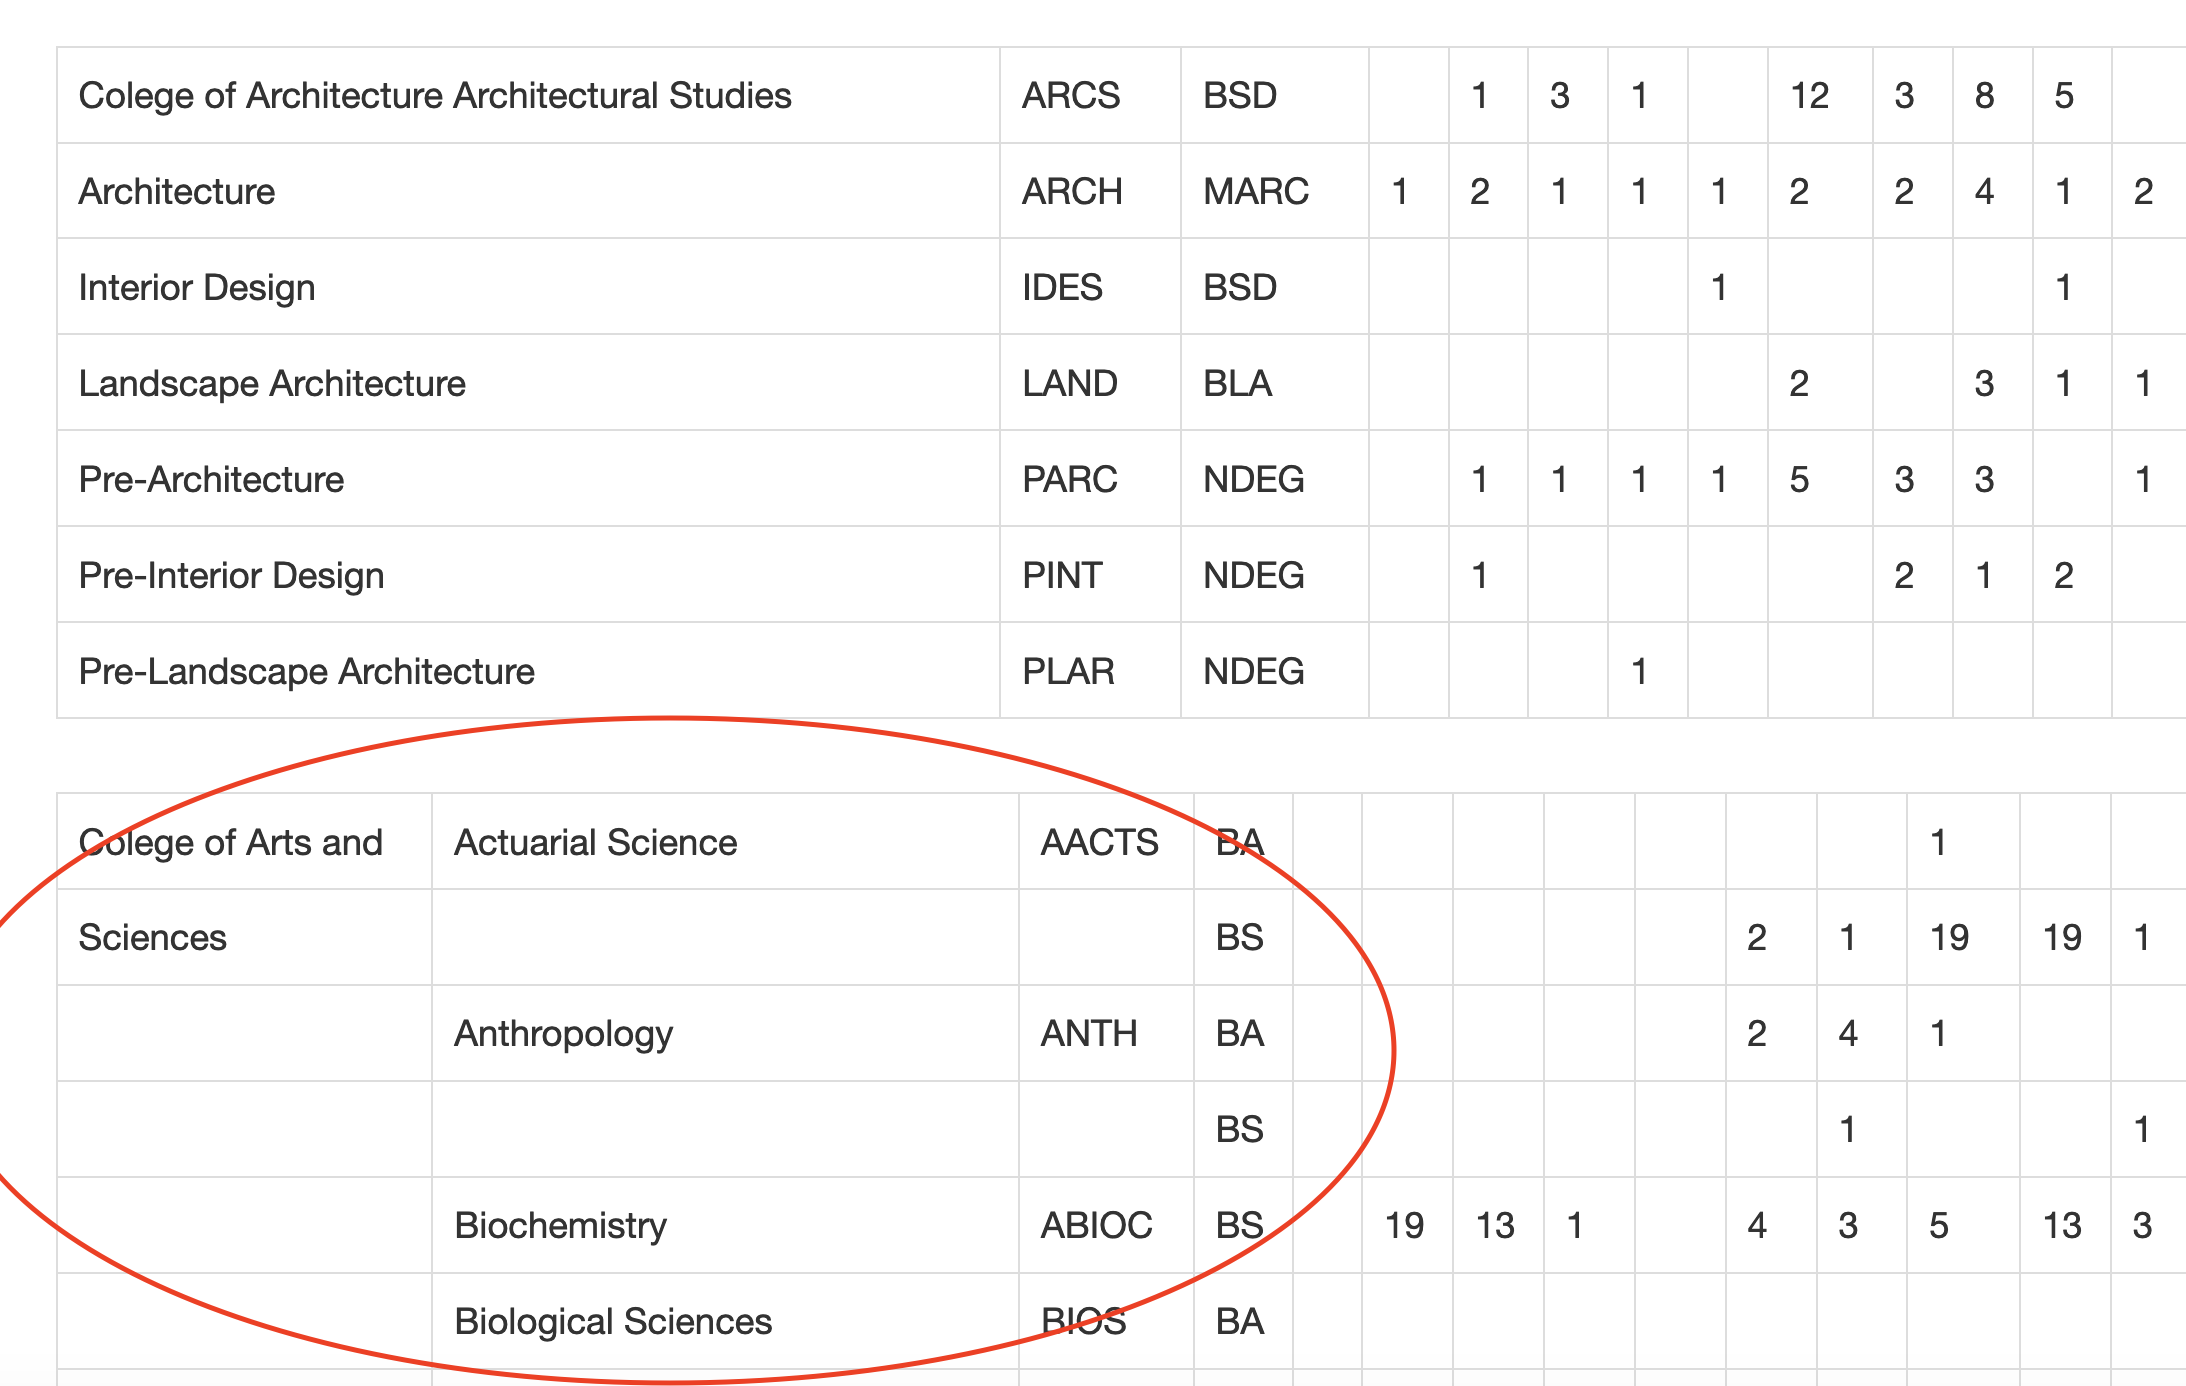
\includegraphics[width=30.36in]{images/pdfs4}

Notice Architecture has the same merging of college name and first major problems as the first one does, but note the blank column is missing.

Look at Arts and Sciences. Arts and Sciences are now in their own column, as the data shows, but there's now empty names that shouldn't be. What are those?

In short, it's a mess.

Here's the sad truth: THIS IS PRETTY GOOD. Open it in a spreadsheet and a little copying and pasting work while double checking the right names line up with the right rows and you're in business. As converted PDFs, this isn't bad.

It beats typing it out.

\hypertarget{when-it-works-well.}{%
\section{When it works well.}\label{when-it-works-well.}}

Each month, the Nebraska Department of Revenue releases the monthly tax receipts of the state, and forecasts into the future what tax receipts might be in the near future. They do this for planning purposes -- the Legislature needs to know how much money the state may have when the new budget is put into place so they know how much money they have to spend.

\href{https://revenue.nebraska.gov/about/news-releases/previous-general-funds-receipts-news-releases}{The announcement comes in a press release}. Each press release includes a table showing the current number, the predicted number, and difference. Of course it's a PDF.

Let's look at the most recent month as of this writing: \href{https://revenue.nebraska.gov/sites/revenue.nebraska.gov/files/doc/news-release/gen-fund/2020/General_Fund_Receipts_January_2020.pdf}{January 2020}. Download it, open it in Tabula and hit Autodetect tables.

You'll note it finds no tables on the first page. Which is good, because there aren't any. Let's look at the third page. It finds a table, but is it one?

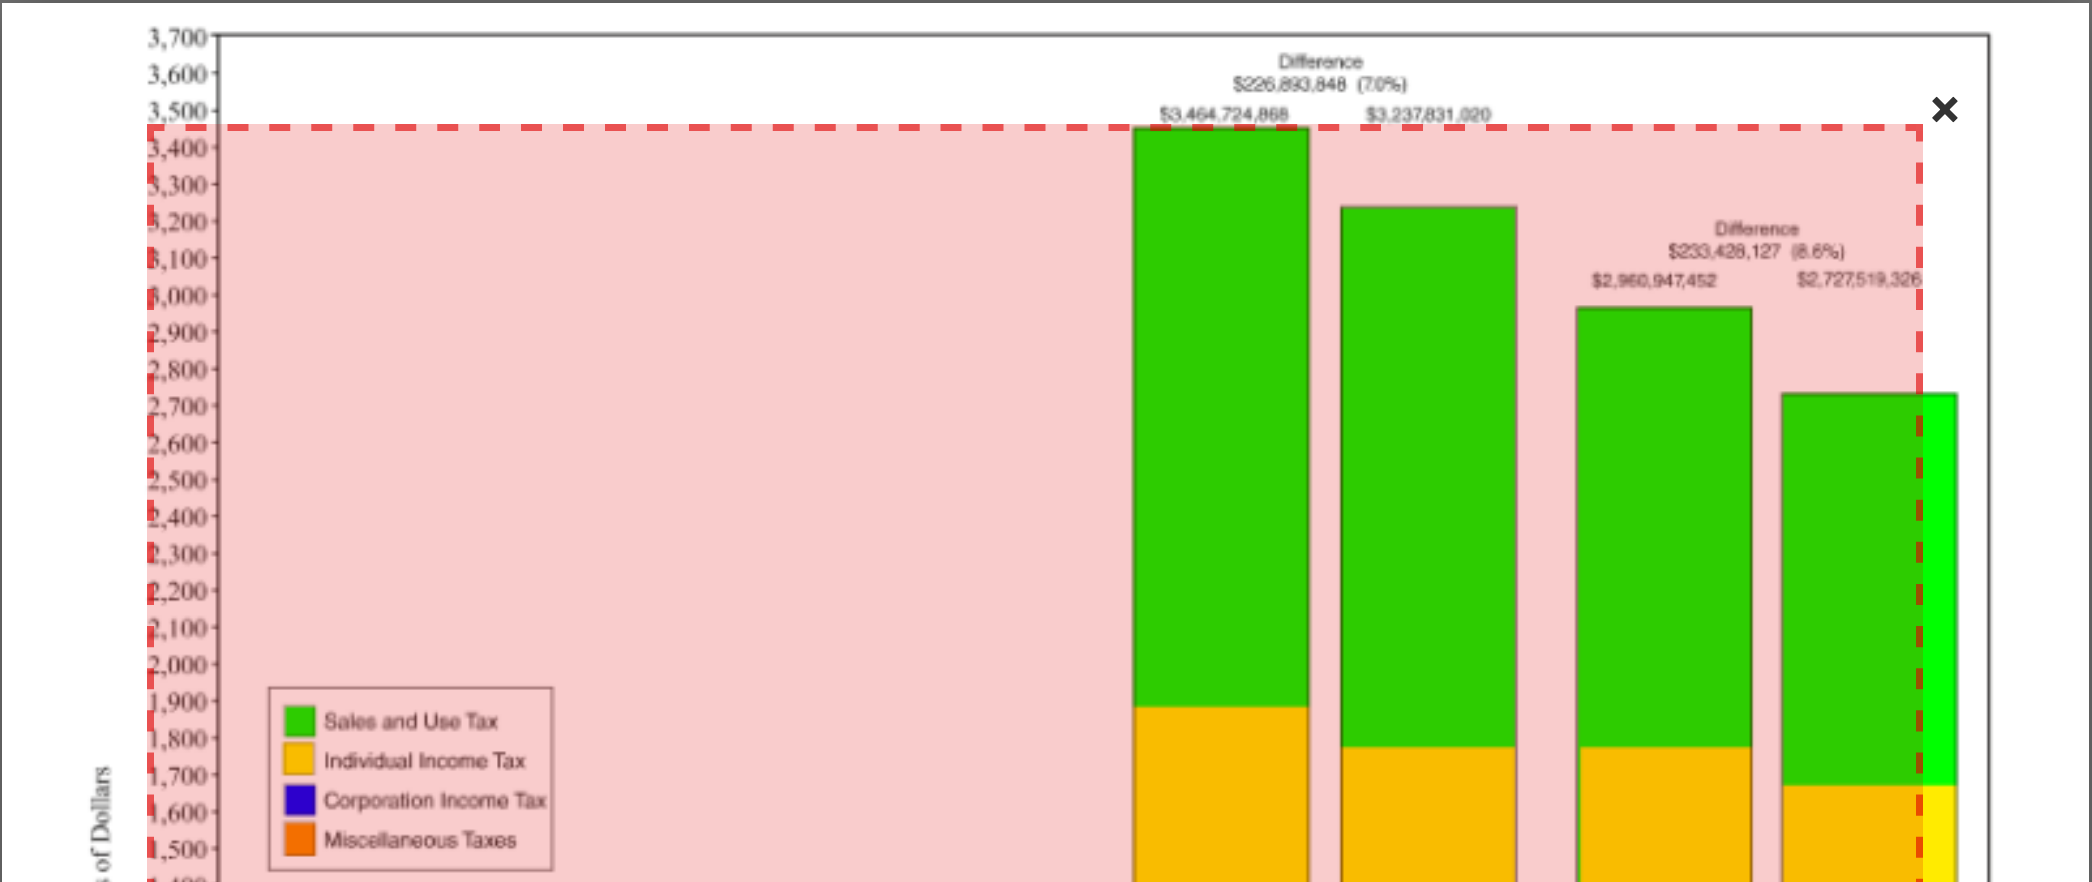
\includegraphics[width=29.06in]{images/pdfs5}

Let's hit the X in the top right on that one.

That leaves page 2. It finds two tables there. Let's just grab the first. Hit X on the second and click to preview the extracted data.

This looks good. So let's export it to a csv.

\hypertarget{cleaning-up-the-data-in-r}{%
\section{Cleaning up the data in R}\label{cleaning-up-the-data-in-r}}

The good news is that we have data we don't have to retype. The bad news is, it's hardly in importable shape.

Let's load libraries.

\begin{Shaded}
\begin{Highlighting}[]
\KeywordTok{library}\NormalTok{(tidyverse)}
\end{Highlighting}
\end{Shaded}

To import this, we need one row of headers. We have three. And we need headers that make sense.

We can spell these out in the import step. First, we'll use \texttt{skip} to skip the first three lines. Then we'll spell out the column names by hand in a \texttt{col\_names} bit. Here's how it looks.

\begin{Shaded}
\begin{Highlighting}[]
\NormalTok{receipts <-}\StringTok{ }\KeywordTok{read_csv}\NormalTok{(}\StringTok{"~/Downloads/tabula-General_Fund_Receipts_January_2020.csv"}\NormalTok{, }\DataTypeTok{skip =} \DecValTok{3}\NormalTok{, }\DataTypeTok{col_names =} \KeywordTok{c}\NormalTok{(}\StringTok{"Month"}\NormalTok{, }\StringTok{"TotalActualNetReceipts"}\NormalTok{, }\StringTok{"TotalProjectedNetReceipts"}\NormalTok{, }\StringTok{"Difference"}\NormalTok{, }\StringTok{"PercentDifference"}\NormalTok{, }\StringTok{"CumulativeActualNetReceipts"}\NormalTok{, }\StringTok{"CumulativeProjectedNetReceipts"}\NormalTok{, }\StringTok{"CumulativeDifference"}\NormalTok{,}\StringTok{"CumulativePercentDifference"}\NormalTok{))}
\end{Highlighting}
\end{Shaded}

\begin{verbatim}
## Parsed with column specification:
## cols(
##   Month = col_character(),
##   TotalActualNetReceipts = col_character(),
##   TotalProjectedNetReceipts = col_character(),
##   Difference = col_character(),
##   PercentDifference = col_character(),
##   CumulativeActualNetReceipts = col_character(),
##   CumulativeProjectedNetReceipts = col_character(),
##   CumulativeDifference = col_character(),
##   CumulativePercentDifference = col_character()
## )
\end{verbatim}

Now we have a harder part.

The columns come in as character columns. Why? Because the state puts commas and \$ and \% in them, which R does not interpret as anything except text. So we need to get rid of them. We can mutate columns and use a function called \texttt{gsub} that finds a string and replaces it with something. So in our case, we're going to \texttt{gsub(",","",\ fieldname)}. The unfortunate part is we have a lot of colunns and a lot of fixes. So this is going to require a lot of code. It is repetitive, though, so we can copy and paste and adjust with most of it.

At the end, we need to use a function called \texttt{mutate\_at} and convert the columns that aren't text into numbers.

And one last thing: If we do many months of this, we should note which report this comes from. We can do this with mutate as well.

Here's what that looks like:

\begin{Shaded}
\begin{Highlighting}[]
\NormalTok{receipts }\OperatorTok\StringTok{ }\KeywordTok{mutate}\NormalTok{(}
  \DataTypeTok{TotalActualNetReceipts =} \KeywordTok{gsub}\NormalTok{(}\StringTok{","}\NormalTok{,}\StringTok{""}\NormalTok{,TotalActualNetReceipts),}
  \DataTypeTok{TotalActualNetReceipts =} \KeywordTok{gsub}\NormalTok{(}\StringTok{"}\CharTok{\textbackslash{}\textbackslash{}}\StringTok{$"}\NormalTok{,}\StringTok{""}\NormalTok{,TotalActualNetReceipts),}
  \DataTypeTok{TotalProjectedNetReceipts =} \KeywordTok{gsub}\NormalTok{(}\StringTok{","}\NormalTok{,}\StringTok{""}\NormalTok{,TotalProjectedNetReceipts),}
  \DataTypeTok{TotalProjectedNetReceipts =} \KeywordTok{gsub}\NormalTok{(}\StringTok{"}\CharTok{\textbackslash{}\textbackslash{}}\StringTok{$"}\NormalTok{,}\StringTok{""}\NormalTok{,TotalProjectedNetReceipts),}
  \DataTypeTok{Difference =} \KeywordTok{gsub}\NormalTok{(}\StringTok{","}\NormalTok{,}\StringTok{""}\NormalTok{,Difference),}
  \DataTypeTok{Difference =} \KeywordTok{gsub}\NormalTok{(}\StringTok{"}\CharTok{\textbackslash{}\textbackslash{}}\StringTok{$"}\NormalTok{,}\StringTok{""}\NormalTok{,Difference),}
  \DataTypeTok{PercentDifference =} \KeywordTok{gsub}\NormalTok{(}\StringTok{"}\CharTok{\textbackslash{}\textbackslash{}}\StringTok{%"}\NormalTok{,}\StringTok{""}\NormalTok{,PercentDifference),}
  \DataTypeTok{CumulativeActualNetReceipts =} \KeywordTok{gsub}\NormalTok{(}\StringTok{","}\NormalTok{,}\StringTok{""}\NormalTok{,CumulativeActualNetReceipts),}
  \DataTypeTok{CumulativeActualNetReceipts =} \KeywordTok{gsub}\NormalTok{(}\StringTok{"}\CharTok{\textbackslash{}\textbackslash{}}\StringTok{$"}\NormalTok{,}\StringTok{""}\NormalTok{,CumulativeActualNetReceipts),}
  \DataTypeTok{CumulativeProjectedNetReceipts =} \KeywordTok{gsub}\NormalTok{(}\StringTok{","}\NormalTok{,}\StringTok{""}\NormalTok{,CumulativeProjectedNetReceipts),}
  \DataTypeTok{CumulativeProjectedNetReceipts =} \KeywordTok{gsub}\NormalTok{(}\StringTok{"}\CharTok{\textbackslash{}\textbackslash{}}\StringTok{$"}\NormalTok{,}\StringTok{""}\NormalTok{,CumulativeProjectedNetReceipts),}
  \DataTypeTok{CumulativeDifference =} \KeywordTok{gsub}\NormalTok{(}\StringTok{","}\NormalTok{,}\StringTok{""}\NormalTok{,CumulativeDifference),}
  \DataTypeTok{CumulativeDifference =} \KeywordTok{gsub}\NormalTok{(}\StringTok{"}\CharTok{\textbackslash{}\textbackslash{}}\StringTok{$"}\NormalTok{,}\StringTok{""}\NormalTok{,CumulativeDifference),}
  \DataTypeTok{CumulativePercentDifference =} \KeywordTok{gsub}\NormalTok{(}\StringTok{"}\CharTok{\textbackslash{}\textbackslash{}}\StringTok{%"}\NormalTok{,}\StringTok{""}\NormalTok{,CumulativePercentDifference)}
\NormalTok{  ) }\OperatorTok\StringTok{ }\KeywordTok{mutate_at}\NormalTok{(}\KeywordTok{vars}\NormalTok{(}\OperatorTok{-}\NormalTok{Month), as.numeric) }\OperatorTok\StringTok{ }\KeywordTok{mutate}\NormalTok{(}\DataTypeTok{ReportMonth =} \StringTok{"January 2020"}\NormalTok{)}
\end{Highlighting}
\end{Shaded}

\begin{verbatim}
## # A tibble: 7 x 10
##   Month TotalActualNetR~ TotalProjectedN~ Difference PercentDifferen~
##   <chr>            <dbl>            <dbl>      <dbl>            <dbl>
## 1 July         284883132        271473079   13410054              4.9
## 2 Augu~        462019974        440504016   21515958              4.9
## 3 Sept~        551908013        510286143   41621870              8.2
## 4 Octo~        289723434        266204529   23518905              8.8
## 5 Nove~        431787603        404934524   26853079              6.6
## 6 Dece~        472926836        421455999   51470837             12.2
## 7 Janu~        467698460        412661036   55037424             13.3
## # ... with 5 more variables: CumulativeActualNetReceipts <dbl>,
## #   CumulativeProjectedNetReceipts <dbl>, CumulativeDifference <dbl>,
## #   CumulativePercentDifference <dbl>, ReportMonth <chr>
\end{verbatim}

We can now reuse this with other months after we harvest the data out of it.

\end{document}
